\documentclass[12pt,italian]{report}
\usepackage[T1]{fontenc}
\usepackage{babel}
\usepackage[utf8]{inputenc}
\usepackage{enumitem}
\usepackage{subfiles}
\usepackage{multirow}
\usepackage{color}
\usepackage{titlesec}
\usepackage{longtable}
\usepackage{xcolor,colortbl}
\usepackage[hidelinks]{hyperref}
\usepackage{graphicx}
\usepackage{adjustbox}
\usepackage{amsmath}
\usepackage{mdframed}
\usepackage{listings}
\usepackage{minted}
\usepackage{subcaption}
\usepackage{changepage}
\usepackage{fancyhdr}

\usepackage[a4paper,right=25mm,top=25mm,bottom=25mm,left=25mm]{geometry}
\usepackage{afterpage}
\usepackage{array,ragged2e}
\usepackage{booktabs}
\usepackage{csquotes}
\usepackage{sectsty}
\usepackage{wrapfig}

\graphicspath{
  {./immagini/}
  {./immagini/icons/}
}

\newcommand\YUGE{\fontsize{33}{25}\selectfont}

\chapternumberfont{\Large} 
\chaptertitlefont{\YUGE}

\titlespacing*{\chapter}
{0pt}{30pt}{35pt}

\titlespacing*{\section}
{0pt}{30pt}{35pt}

\titlespacing*{\subsection}
{0pt}{25pt}{27pt}

\setlength{\parindent}{0cm}
\setlist[itemize]{noitemsep, topsep=0pt}



\newcolumntype{P}[1]{>{\RaggedRight\arraybackslash}p{#1}}
\renewcommand{\baselinestretch}{1.5} 

\newlist{tabitem}{itemize}{1}
\setlist[tabitem]{nosep,
                  topsep     = 0pt,
                  partopsep  = 0pt,
                  leftmargin = *,
                  label      = \textbullet,
                  before = \vspace{-1\baselineskip},
                  after = \vspace{-0.5\baselineskip}}

\hypersetup{
    linktoc=all,
    pdfpagemode=FullScreen,
}


\newcommand{\mycomment}[1]{}

\mycomment{}



\pagestyle{fancy}
\fancyhf{}
\renewcommand{\headrulewidth}{0pt}


\begin{document}

\pagenumbering{gobble}


\begin{titlepage}
    
\pagestyle{empty}
\newgeometry{
    left=20mm,
    right=20mm,
    top=20mm,
    bottom=20mm
}


\begin{center}

% marchio di ateneo

\includegraphics[width=6.5cm,height=4.7cm]{marchio-di-ateneo_gs.png}

\vspace{10mm}

% \large is 12pt
{\normalsize{\bf{DIPARTIMENTO DI INFORMATICA - SCIENZA e INGEGNERIA}}} 

\vspace{5mm}

{\large{\bf{CORSO DI LAUREA MAGISTRALE IN INGEGNERIA INFORMATICA}}}
\end{center}
\vspace{23mm}
\begin{adjustwidth}{15mm}{15mm}
\begin{center}

{\LARGE{\bf Analisi, Progettazione e Distribuzione in Cloud di applicativo multipiattaforma}}\\

{\LARGE{\bf per l'organizzazione di eventi condivisi e la condivisione multimediale automatica in tempo reale}}\\
\vspace{3mm}
%{\Huge{\bf }}\\
\vspace{3mm}

\end{center}
\end{adjustwidth}

\vspace{35mm}

\begin{minipage}[t]{0.40\textwidth}
{\Large{\bf Relatore: \\ Chiar.mo Prof.\\ Michele Colajanni}}

\vspace{3mm}

{\Large{\bf }}
\end{minipage}
\hfill
\begin{minipage}[t]{0.40\textwidth}\raggedleft
{\Large{\bf Presentata da: \\ Giacomo Romanini}}
\end{minipage}

\vspace{10mm}

\rule[0.5cm]{15.8cm}{0.6mm}

\begin{center}
{\large{\bf Sessione Luglio 2025 \\}}
{\large{\bf Anno Accademico 2025/2026\\}}
\end{center}

\end{titlepage}

\restoregeometry

\newpage
\
\newpage

\chapter*{Abstract}


Lo sviluppo di un applicativo multipiattaforma diretto all'organizzazione di eventi condivisi,
caratterizzato in particolare dalla condivisione multimediale in tempo reale,
richiede opportune capacità di scalabilità, 
atte a garantire una risposta efficace anche con alti volumi di richieste, offrendo prestazioni ottimali. 
Le tecnologie cloud, con la loro disponibilità pressoché illimitata di risorse e la completa e continua garanzia  di manutenzione, 
offrono l'architettura ideale per il supporto di simili progetti, anche con fondi limitati.\\
\\
Tuttavia, l'integrazione tra la logica applicativa e i molteplici servizi cloud, 
assieme alla gestione delle loro interazioni reciproche, comporta sfide specifiche, 
in particolare legate all'ottimizzazione di tutte le risorse.
L'individuazione e la selezione delle soluzioni tecnologiche più adatte per ogni funzionalità, 
così come l'adozione delle migliori pratiche progettuali,
devono procedere parallelamente con lo sviluppo del codice, 
al fine di sfruttare efficacemente le potenzialità offerte.\\
\\
In tale prospettiva, 
questa tesi illustra le scelte progettuali e implementative adottate nello sviluppo di Wyd,
applicativo per la condivisione di eventi,
evidenziando l'impatto dell'integrazione delle risorse cloud sul risultato finale.\\
\clearpage

\tableofcontents
\clearpage

\pagenumbering{arabic}
\fancyfoot[C]{\thepage}

\chapter*{Introduzione}
\addcontentsline{toc}{chapter}{Introduzione}


In un contesto sociale sempre più connesso, la crescente quantità di contatti, 
la rapidità delle comunicazioni e l'accesso universale alle informazioni 
rendono la ricerca, l'organizzazione e la partecipazione ad eventi estremamente facile, 
ma al contempo generano un ambiente frenetico e spesso dispersivo.\\
\\
Risulta infatti difficile seguire tutte le opportunità a cui si potrebbe partecipare, 
considerando le numerose occasioni che si presentano quotidianamente. 
Basti pensare, ad esempio, alle riunioni di lavoro, alle serate con amici, agli appuntamenti informali per un caffè, 
ma anche a eventi più strutturati come fiere, convention aziendali, concerti, partite sportive o mostre di artisti che visitano occasionalmente la città.\\
\\
Questi eventi possono sovrapporsi, causando dimenticanze o conflitti di pianificazione, 
con il rischio di delusione o frustrazione. 
Quando si è invitati a un evento, può capitare di essere già impegnati, 
o di trovarsi in attesa di una conferma da parte di altri contatti.
In questi casi, la gestione degli impegni diventa complessa: 
spesso si conferma la partecipazione senza considerare possibili sovrapposizioni, o dimenticandosi, 
per poi dover scegliere e disdire all'ultimo momento. \\
\\
D’altra parte, anche quando si desidera proporre un evento, 
la ricerca di un'attività interessante può diventare un compito arduo, 
con la necessità di consultare numerosi profili social di locali e attività,
senza avere inoltre la certezza che gli altri siano disponibili.
Tali problemi si acuiscono ulteriormente quando si tratta di organizzare eventi di gruppo, 
dove bisogna allineare gli impegni di più persone.\\
\clearpage
In questo contesto, emergono la necessità e l'opportunità di sviluppare uno strumento che semplifichi la proposta e la gestione degli eventi, 
separando il momento della proposta da quello della conferma di partecipazione. 
In tal modo, gli utenti possono valutare la disponibilità degli altri prima di impegnarsi definitivamente, 
facilitando in conteporanea sia l'invito sia la partecipazione.\\ 
\\
In risposta a tali richieste è stata creata Wyd, 
un'applicazione che permette agli utenti di organizzare i propri impegni, 
siano essi confermati oppure proposti. 
Essa permette anche di rendere più intuitiva la ricerca di eventi 
attraverso la creazione di uno spazio virtuale centralizzato 
dove gli utenti possano pubblicare e consultare tutti gli eventi disponibili,
diminuendo l’eventualità di perderne qualcuno.
La funzionalità chiave di questo progetto si fonda sull'idea di affiancare alla tradizionale agenda degli impegni confermati un calendario separato, 
che mostri tutti gli eventi a cui si potrebbe partecipare. \\
\\
\begin{wrapfigure}{r}{0.4\textwidth}
    \centering
    
\includegraphics[height=.3\textheight]{logo.png}
    \caption{Il logo di Wyd}
\end{wrapfigure}	
Una volta confermata la partecipazione a un evento, 
questo verrà spostato automaticamente nell'agenda personale dell'utente.
Gli eventi creati potranno essere condivisi con persone o gruppi, 
permettendo di visualizzare le conferme di partecipazione. 
Considerando l'importanza della condivisione di contenuti multimediali, 
questo progetto prevede la possibilità di condividere foto e video con tutti i partecipanti all'evento, 
attraverso la generazione di link per applicazioni esterne o grazie all'ausilio di gruppi di profili. 
Al termine dell’evento, l'applicazione carica automaticamente le foto scattate durante l'evento,
per allegarle a seguito della conferma dell'utente.



\clearpage
La realizzazione di un progetto come Wyd implica la risoluzione e 
la gestione di diverse problematiche tecniche. 
In primo luogo, la stabilità del programma deve essere garantita 
da un'infrastruttura affidabile e scalabile. 
La persistenza deve essere mantenuta aggiornata e coerente, 
fornendo alte prestazioni sia in lettura che in scrittura indipendentemente dalla quantità delle richieste.
La funzionalità di condivisione degli eventi richiede inoltre l'aggiornamento in tempo reale verso tutti gli utenti coinvolti.
Infine, il caricamento ed il salvataggio delle foto aggiungono la necessità di gestire richieste di archiviazione di dimensioni significative.\\
\\
\section*{Organizzazione dei capitoli}
\addcontentsline{toc}{section}{Organizzazione dei capitoli}

Il seguente elaborato è suddiviso in cinque capitoli.\\
Nel primo capitolo si affronta la fase di analisi delle funzionalità,
durante la quale, partendo dall'idea astratta iniziale,
si definiscono i requisiti e le necessità del sistema,
per poi creare la struttura generale ad alto livello dell'applicazione.\\
Nel secondo capitolo si affrontano le principali scelte architetturali e di sviluppo
che hanno portato a definire la struttura centrale dell’applicazione.\\
Il terzo capitolo osserva lo studio effettuato per gestire la memoria, 
in quanto fattore che più incide sulle prestazioni. 
Particolare attenzione è stata dedicata, infatti, 
a determinare le tecnologie e i metodi che meglio corrispondono alle esigenze 
derivate dal salvataggio e dall’interazione logica degli elementi.\\
Il quarto capitolo si concentra sulle scelte implementative adottate 
per l’inserimento le funzionalità legate alla gestione delle immagini,
che, oltre ad introdurre problematiche impattanti sia sulle dimensioni delle richieste 
sia sull'integrazione con la persistenza, 
richiedono l'automatizzazione del recupero delle immagini.\\
Infine, nel quinto capitolo, verranno analizzati e discussi i risultati ottenuti
testando il sistema.


\clearpage


\renewcommand\chaptermark[1]{\markboth{\thechapter\,--\,#1}{}}
\fancyhead[L]{\leftmark}

%\chapter{Analisi delle funzionalità}

La realizzazione di qualunque prodotto software inizia da una fase in cui,
partendo dall’abstract del progetto, si analizzano i requisiti e le funzionalità da realizzare.
L’obiettivo è arrivare a una definizione delle proprietà e
del comportamento desiderato nell’applicazione che sia concisa e condivisa col cliente,
senza però entrare nel merito delle scelte implementative.\\
Solo a quel punto si può procedere con lo sviluppo del programma vero e proprio.\\
\\
L'abstract di Wyd è il seguente:\\
\\
Wyd è un'applicazione che permette ai clienti di organizzare i propri impegni,
siano essi confermati oppure proposti.
Mette a disposizione due calendari,
il primo con gli eventi in cui l'utente è convinto di partecipare,
il secondo in cui vengono riuniti gli eventi a cui l'utente è stato invitato ma senza aver ancora dato conferma.
L'utente ha la possibilità di creare, modificare, confermare o disdire un evento,
ma anche condividerlo con altri o allegarci foto.\\
\\
La condivisione di un evento può avvenire con applicazioni esterne tramite la generazione di un link o
grazie all'ausilio di gruppi di profili.
Inoltre, al termine di un evento, l'applicazione carica automaticamente le foto scattate
durante l'evento, per allegarle a seguito della conferma dell'utente.
L'utente può infatti cercare altri profili e creare gruppi con i profili trovati.
Tutta l'interazione avviene tramite l'utilizzo di profili,
che permettono di suddividere semanticamente gli eventi e le relazioni.
\clearpage

\section{L'individuazione dei requisiti e dei casi d’uso}

Lo studio dell’abstract del progetto porta all’individuazione e
alla descrizione delle sue caratteristiche essenziali.
In particolare, si distinguono i requisiti e i casi d'uso.
I requisiti formalizzano le funzionalità che l'applicazione deve fornire,
sintetizzando e schematizzando le parti che descrivono del prodotto.
I casi d'uso descrivono invece le interazioni previste tra l'utente e il sistema,
suddividendo le funzionalità in azioni elementari.\\
\subsection{I requisiti e il vocabolario}
I requisiti devono risultare chiari e precisi
per permettere di procedere alle fasi successive in maniera corretta e trasparente.
Ogni requisito deve essere breve e puntuale, limitato a un solo particolare desiderata,
focalizzando una necessità specifica.\\
Si suddividono in funzionali o non funzionali in base alle loro caratteristiche.
I requisiti funzionali descrivono le funzionalità che il sistema deve fornire,
mentre i requisiti non funzionali illustrano le caratteristiche che il sistema deve soddisfare per essere considerato valido.\\
\\
Da una prima analisi dell'abstract si evincono immediatamente i principali requisiti funzionali,
che riguardano in generale l'esperienza utente nelle sue parti principali,
dalla visualizzazione nelle schermate all'inserimento di dati e foto.
Si aggiungono quindi le funzionalità dettate da necessità derivate,
quali l'esigenza di autenticare l'utente o il bisogno di gestire i profili e i gruppi.
Infine si analizzano le specifiche non funzionali,
che sono raramente incluse nel testo ma che descrivono le caratteristiche performative e di sicurezza
ritenute essenziali per il successo desiderato.\\
\\
Vengono quindi introdotti i desiderata relativi all'esperienza utente,
evidenziando l'intuitività e la reattività dell'applicazione,
che richiedono di conseguenza velocità nel recuperare i dati.
Inoltre, essendo Wyd pensata per interagire con migliaia di utenti,
in simultanea e interconnessi tra loro, le caratteristiche di scalabilità vengono individuate e introdotte fin da subito.
La sicurezza del sistema, escludendo l'autenticazione che impatta direttamente sull'utente,
necessitando di un'analisi approfondita apposita, viene trattata in seguito.\\

\begin{longtable} {|P{1.3cm}|P{11.2cm}|P{3cm}|}
    \hline
    \textbf{ID} & \textbf{Requisiti}                                                         & \textbf{Tipo}  \\
    \hline
    \endhead
    R1F         & Registrazione di un account tramite l’interfaccia web                      & Funzionale     \\
    \hline
    R2F         & Identificazione attraverso mail univoca e password di almeno sei caratteri & Funzionale     \\
    \hline
    R3F         & Visualizzazione degli eventi confermati                                    & Funzionale     \\
    \hline
    R4F         & Visualizzazione degli eventi proposti                                      & Funzionale     \\
    \hline
    R5F         & Creazione di un evento impostando almeno la data d'inizio e quella di fine & Funzionale     \\
    \hline
    R6F         & La data di fine deve essere successiva alla data d'inizio                  & Funzionale     \\
    \hline
    R7F         & Modifica di un evento                                                      & Funzionale     \\
    \hline
    R8F         & La conferma di un evento lo sposta negli eventi confermati                 & Funzionale     \\
    \hline
    R9F         & La disdetta di un evento lo sposta negli eventi proposti                   & Funzionale     \\
    \hline
    R10F        & Caricamento delle foto di un evento                                        & Funzionale     \\
    \hline
    R11F        & Condivisione tramite link                                                  & Funzionale     \\
    \hline
    R12F        & Condivisione tramite gruppo o ad altri profili                             & Funzionale     \\
    \hline
    R13F        & Ricerca automatica delle foto sul dispositivo mobile                       & Funzionale     \\
    \hline
    R14F        & Conferma delle foto                                                        & Funzionale     \\
    \hline
    R15F        & Ricerca di altri profili                                                   & Funzionale     \\
    \hline
    R16F        & Creazione di un gruppo da due o più profili                                & Funzionale     \\
    \hline
    R17F        & Visualizzazione dei profili collegati                                      & Funzionale     \\
    \hline
    R18F        & Creazione di un nuovo profilo                                              & Funzionale     \\
    \hline
    R19F        & Cambio del profilo attualmente in uso                                      & Funzionale     \\
    \hline
    R20F        & Aggiornamento in tempo reale delle modifiche agli eventi                   & Funzionale     \\
    \hline
    R1NF        & Per interagire l'utente deve essere autenticato                            & Non Funzionale \\
    \hline
    R2NF        & Velocità di richiesta iniziale dei dati                                    & Non Funzionale \\
    \hline
    R3NF        & Semplicità e fluidità dell'interfaccia grafica                             & Non Funzionale \\
    \hline
    R4NF        & Velocità in lettura e scrittura dei dati                                   & Non Funzionale \\
    \hline
    R5NF        & Velocità nella ricerca dei profili                                         & Non Funzionale \\
    \hline
    R6NF        & Scalabilità delle richieste                                                & Non Funzionale \\
    \hline
    \caption{Tabella dei requisiti di Wyd}
\end{longtable}


Alla tabella dei requisiti si affianca quella del vocabolario,
definendo i termini utilizzati nel progetto per allinearli definitivamente alle volontà del cliente.
Questo consentirà, quando in seguito verranno citati,
di evitare possibili ambiguità derivate dall'uso comune dei termini.
Si specifica cosa si intende quindi per utente, profilo e gruppo, ma anche,
analizzando i requisiti circoscritti in precedenza,
evento confermato e proposto, o ancora email e password.
\\

\begin{longtable} {|P{3.5cm}|P{9cm}|P{3cm}|}
    \hline
    \textbf{Voce}     & \textbf{Definizione}                                                             & \textbf{Sinonimi}                 \\
    \hline
    \endhead
    Account           & combinazione di mail e password che identifica un utente                         &                                   \\
    \hline
    Utente            & Persona che utilizza l'applicazione                                              &                                   \\
    \hline
    Profilo           & Entità logica che raggruppa eventi e interazioni                                 &                                   \\
    \hline
    Profili collegati & Profili a cui l'utente può avere accesso                                         &                                   \\
    \hline
    Gruppo            & Insieme di profili                                                               &                                   \\
    \hline
    Evento            & Azione(o previsione di azione) con una durata nel tempo                          &                                   \\
    \hline
    Data e ora evento & Indicazione temporale del momento in cui avverrà l'azione                        &                                   \\
    \hline
    Evento confermato & Evento a cui il profilo ha dato conferma di partecipazione                       &                                   \\
    \hline
    Evento proposto   & Evento a cui il profilo non ha dato conferma di partecipazione                   & Evento disdetto, evento condiviso \\
    \hline
    Email             & Indirizzo di posta elettronica del cliente utilizzata anche per l'autenticazione &                                   \\
    \hline
    Password          & Codice alfanumerico di almeno otto caratteri                                     &                                   \\
    \hline
    Credenziali       & Insieme composto da email e password necessari per accedere al sistema           &                                   \\
    \hline
    \caption{Vocabolario di Wyd}
\end{longtable}


\subsection{I casi d’uso}

I casi d’uso descrivono le interazioni tra gli attori e il sistema,
suddividendo le funzionalità in azioni elementari.
Si definiscono attori tutti gli elementi che compiono una parte attiva nei confronti del programma.
Ogni attore può interagire con uno o più casi d'uso,
e ogni caso d'uso può essere relazionato con altri, definendo la loro relazione.\\
\\
I casi d'uso possono essere collegati tra loro tramite rapporti d'inclusione o estensione.
Si dice che un caso include un altro se contiene il suo comportamento.
Si dice invece che un caso d'uso ne estende un altro se
il suo comportamento può essere inserito all'interno del secondo.\\
\\
Per ogni azione descritta nei requisiti, intuibile dal contesto o necessaria per il soddisfacimento dei requisiti,
viene introdotto un nuovo caso d'uso.
Ad esempio, la creazione o la condivisione di un evento
vengono estratti direttamente dalla descrizione del progetto,
così come la ricerca automatica delle immagini.
L'eliminazione di un evento, la registrazione di un utente o l'aggiunta di un profilo a un gruppo,
per quanto non espressamente elencati tra i requisiti,
sono dedotti dal contesto.
L'aggiornamento da un server esterno viene introdotto
per realizzare la modifica in tempo reale degli eventi.\\
\\
I casi d'uso così individuati si raggruppano attorno a tre principali.
VisualizzaEvento permette di visualizzare i dettagli dell'evento,
ma anche di modificarli e di eseguire tutte le azioni relative.
GestioneGruppi racchiude tutte le esigenze che riguardano i contatti e i gruppi,
come la visualizzazione dei gruppi, la ricerca dei profili e l'aggiunta di un profilo a un gruppo.
Infine GestioneProfili permette il controllo dei profili collegati all'utente,
visualizzandoli e dando la possibilità di cambiare il profilo corrente.\\
\\
Si distinguono rispetto ai precedenti casi d'uso e alle loro estensioni
altre funzionalità il cui scopo non riguarda nessuno dei tre argomenti,
o il cui funzionamento sia scorrelato.
Login e Registrazione, ad esempio,
vedono il loro utilizzo in maniera trasversale rispetto al resto dell'applicazione,
essendo necessari per il funzionamento di tutti ma distanti da un punto di vista logico.
AggiornaEvento e RecuperaImmagini eseguono indipendentemente dall'interazione utente,
apportando modifiche automaticamente in base ad attori esterni.\\

\begin{figure}[htb]
    \centering
    \adjustbox{width=\textwidth}{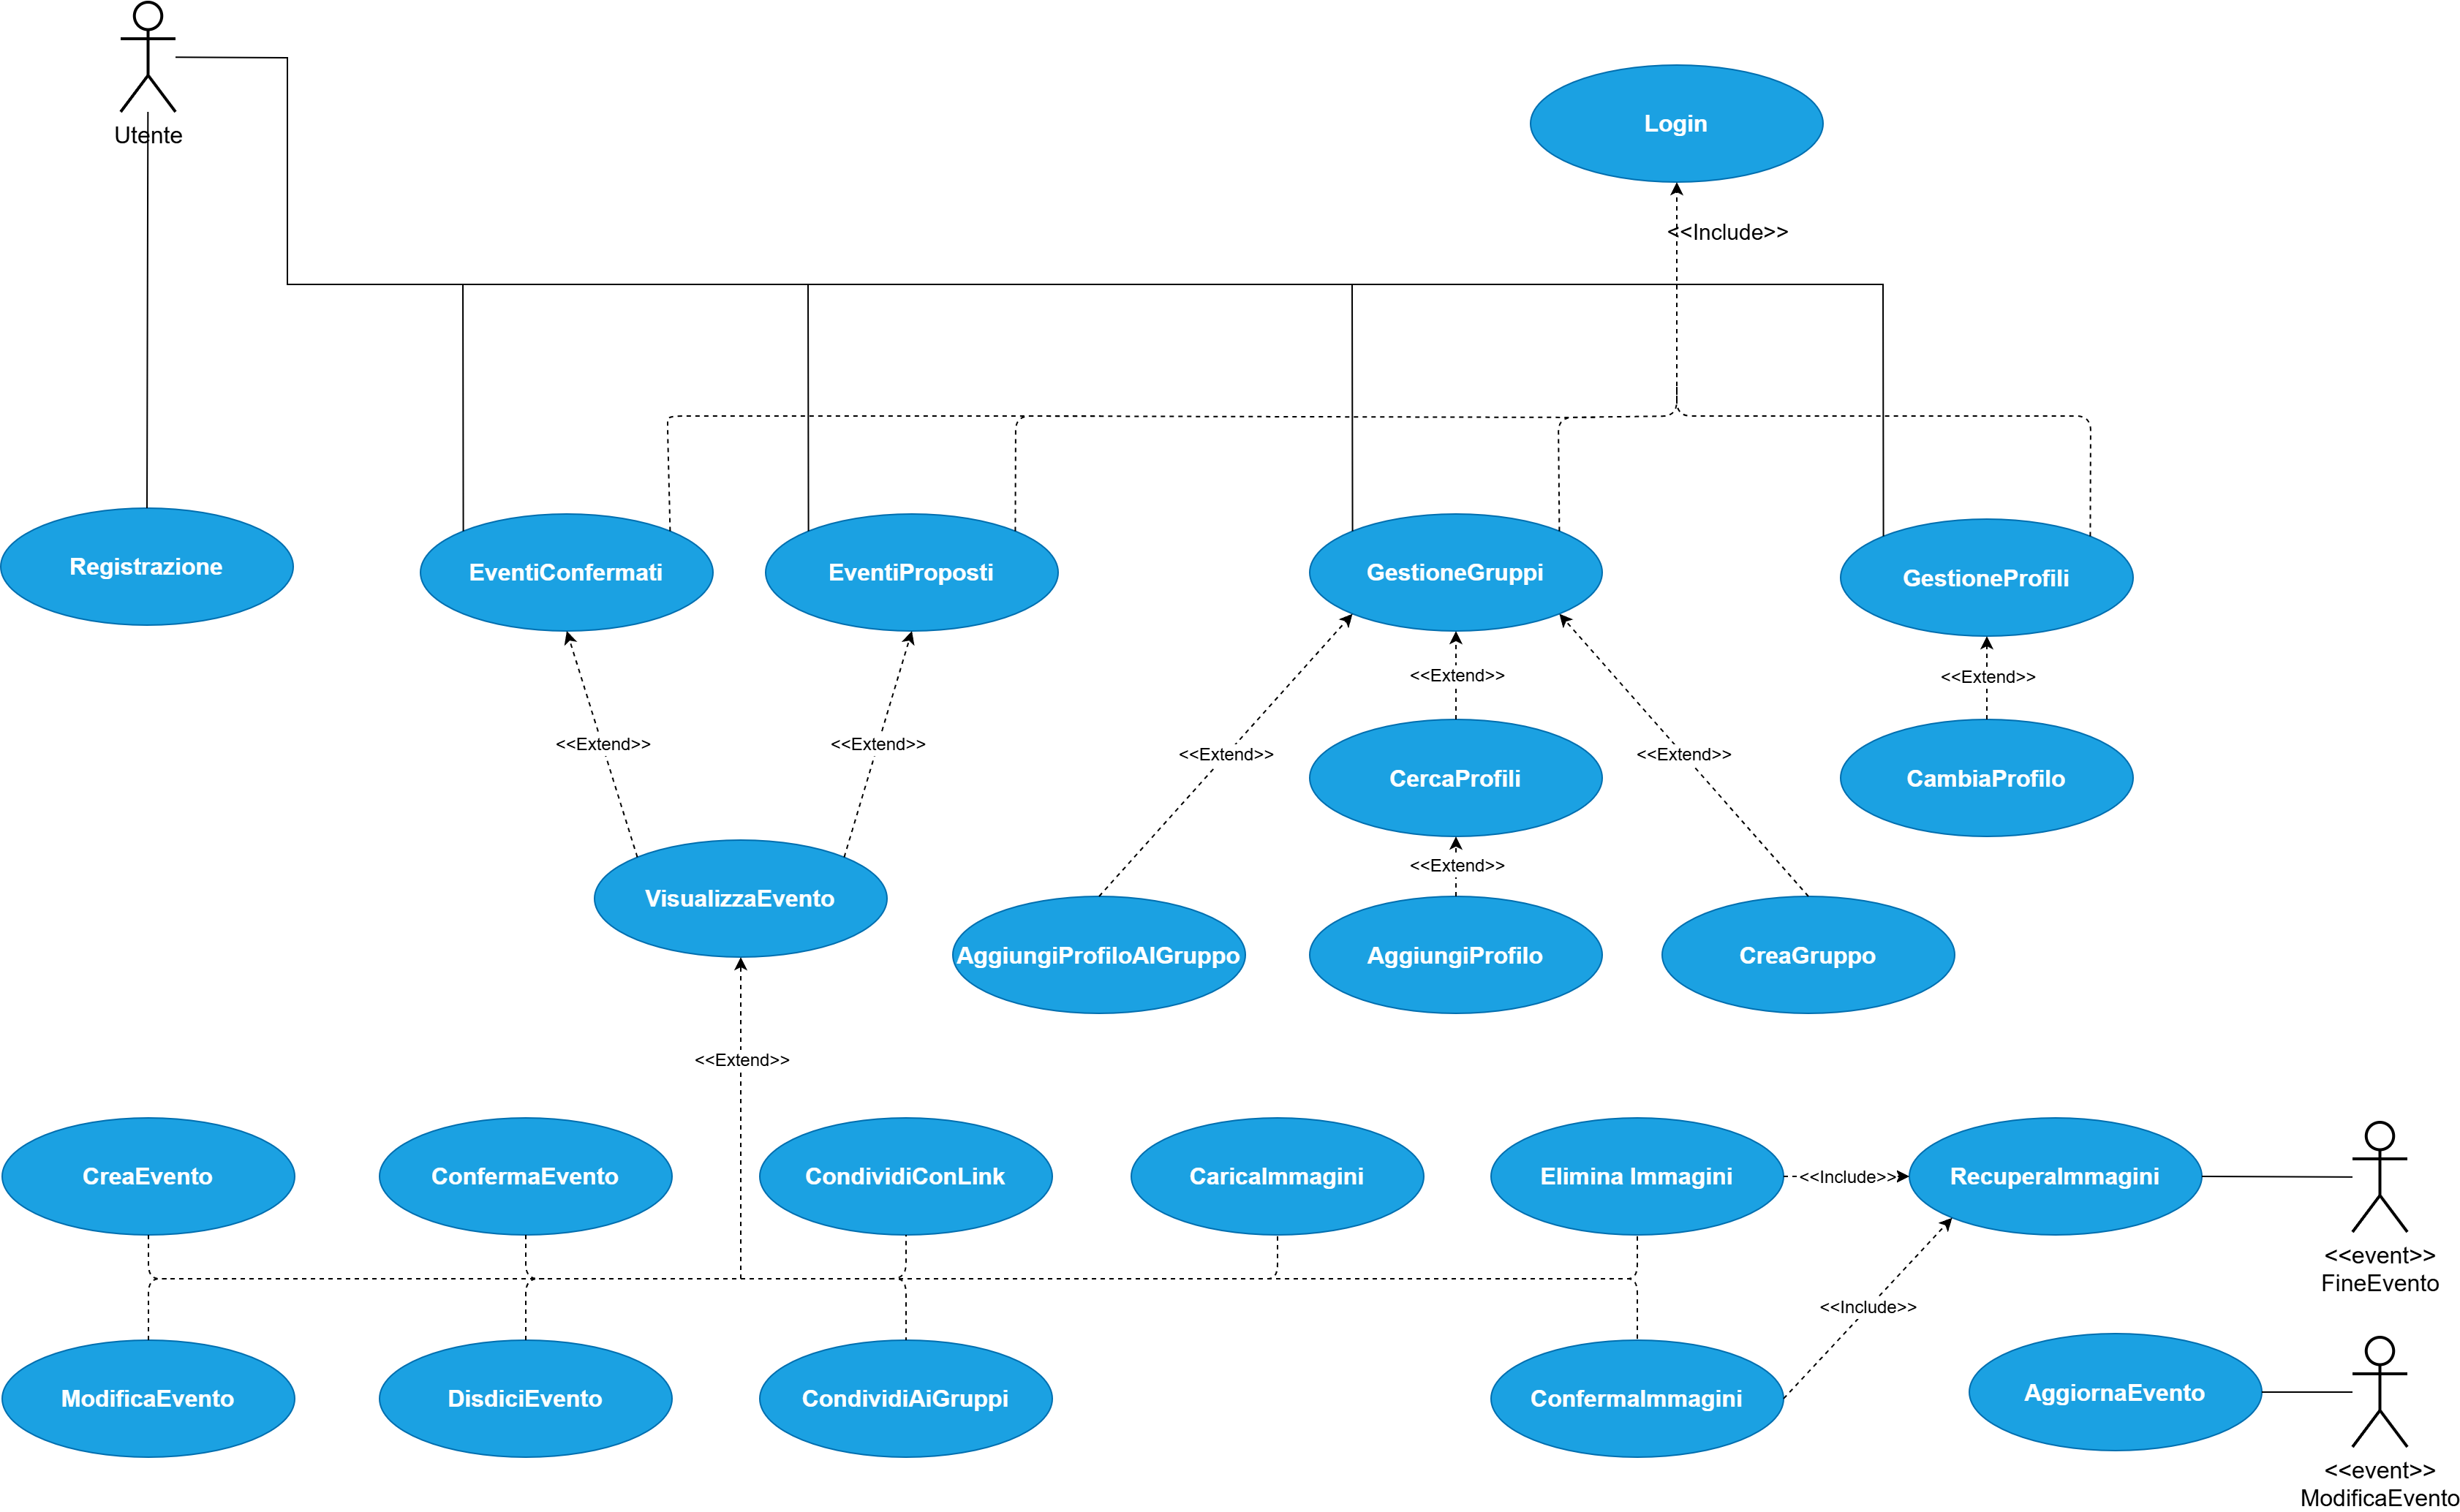
\includegraphics{Casiduso.png}}
    \caption{Diagramma dei casi d'uso}
\end{figure}

Per ogni caso d'uso viene poi identificato uno scenario di utilizzo,
che chiarifica il contesto, il comportamento e i punti critici dell'utilizzo.
Lo scenario ha il solo compito di mostrare il comportamento desiderato,
senza scendere quindi in dettagli o complessità progettuali.
Dallo scenario risulta quindi complesso dedurre la difficoltà implementativa del caso d'uso,
ma è il tassello da cui si stabiliranno poi la coordinazione e l'interazione delle varie parti del programma.\\
\\
Si riportano gli scenari di utilizzo per i principali casi d'uso di Wyd,
ovvero quelli che più andranno a impattare sulla struttura e sulle esigenze del progetto.\\
\\
Lo scenario di registrazione vede la responsabilità, oltre che di creare un account,
di collegare un profilo all'utente.
Questa separazione consente di avere una struttura gerarchica
che permette di associare più profili a un unico utente,
che può così in seguito crearne o unirne di nuovi.\\

\begin{longtable} {|P{4.5cm}|P{11cm}|}
    \hline
    \textbf{Titolo}                   & Registrazione                                                                         \\
    \hline
    \textbf{Descrizione}              & L'utente si registra al servizio                                                      \\
    \hline
    \textbf{Attori}                   & Utente                                                                                \\
    \hline
    \textbf{Relazioni}                &                                                                                       \\
    \hline
    \textbf{Precondizioni}            &                                                                                       \\
    \hline
    \textbf{Post condizioni}          & L'utente è registrato nel sistema e può interagire con il resto dell'applicazione     \\
    \hline
    \textbf{Scenario principale}      & 1.L'utente accede alla schermata di registrazione      \newline
    2. L'utente inserisce email e  password                      \newline
    3. Il sistema crea un account con le credenziali inserite, associando un utente e un primo profilo   \newline
    4. L'utente termina la registrazione, se avvenuta con successo viene reindirizzato alla pagina principale
    \\
    \hline
    \textbf{Scenari Alternativi}      &

    Il sistema verifica che è già presente un account con la mail inserita, quindi procede con la procedura di login normale. \\
    \hline
    \textbf{Requisiti non funzionali} &
    Per interagire l'utente deve essere autenticato \newline
    Velocità in lettura e scrittura dei dati                                                                                  \\
    \hline
    \textbf{Punti aperti}             &                                                                                       \\
    \hline
    \caption{Scenario di registrazione}
\end{longtable}

A seguito della modifica di un evento,
che implica il salvataggio dei suoi nuovi dati,
viene chiesto l'aggiornamento in tempo reale verso
tutti i dispositivi di tutti gli utenti a cui l'evento è stato condiviso.
Inoltre, sarà necessario inserire un controllo per evitare
che due richieste simultanee causino conflitti.\\

\begin{longtable} {|P{4.5cm}|P{11cm}|}
    \hline
    \textbf{Titolo}                   & ModificaEvento                                                                               \\
    \hline
    \textbf{Descrizione}              & Salva le modifiche a un evento                                                               \\
    \hline
    \textbf{Attori}                   & Utente                                                                                       \\
    \hline
    \textbf{Relazioni}                & VisualizzaEvento                                                                             \\
    \hline
    \textbf{Precondizioni}            & L'evento esiste e sono stati modificati dei dati                                             \\
    \hline
    \textbf{Post condizioni}          & Le modifiche vengono salvate e propagate a tutti i profili collegati                         \\
    \hline
    \textbf{Scenario Principale}      & 1. VisualizzaEvento \newline
    2. Il sistema controlla che i dati modificati siano corretti\newline
    3. I cambiamenti vengono salvati\newline
    4. Tutti i dispositivi collegati ai profili collegati all'evento visualizzano le immagini                                        \\
    \hline
    \textbf{Scenari Alternativi}      & 2. Se i dati risultano sbagliati, il sistema notifica l'utente originario indicando l'errore \\
    \hline
    \textbf{Requisiti non funzionali} & Velocità in lettura e scrittura dei dati \newline
    Scalabilità delle richieste                                                                                                      \\
    \hline
    \textbf{Punti aperti}             & Le modifiche all'evento devono essere consistenti, \newline
    soprattutto in caso di richieste simultanee                                                                                      \\
    \hline
    \caption{Scenario della modifica di un evento}
\end{longtable}

Il salvataggio delle immagini è un'operazione di particolare importanza
vista la sua rilevanza nel coinvolgimento degli utenti
nell'utilizzo delle funzionalità centrali dell'applicazione,
e quindi nel successo del progetto.
Oltre a mostrare un'interfaccia intuitiva,
il sistema deve essere in grado di gestire queste particolari richieste di caricamento,
che generalmente necessitano di più tempo e memoria.
Prevedendo che la maggior parte di queste avvenga in seguito alla conclusione dell'evento,
la probabilità che più richieste simultanee vertano sullo stesso evento risulta elevata,
creando la necessità di una gestione parallela di modifiche concorrenti.\\

\begin{longtable} {|P{4.5cm}|P{11cm}|}
    \hline
    \textbf{Titolo}                   & CaricaImmagini                                                                  \\
    \hline
    \textbf{Descrizione}              & Permette all'utente di selezionare immagini da collegare all'evento, salvandole \\
    \hline
    \textbf{Attori}                   & Utente                                                                          \\
    \hline
    \textbf{Relazioni}                & VisualizzaEvento                                                                \\
    \hline
    \textbf{Precondizioni}            & L'evento esiste                                                                 \\
    \hline
    \textbf{Post condizioni}          & Le immagini vengono salvate e propagate a tutti i profili collegati             \\
    \hline
    \textbf{Scenario Principale}      & 1. VisualizzaEvento \newline
    2. L'utente seleziona le immagini che vuole caricare\newline
    3. Le immagini vengono salvate\newline
    4. Tutti i dispositivi relativi ai profili collegati all'evento visualizzano le immagini                            \\
    \hline
    \textbf{Scenari Alternativi}      &
    Scenario alternativo A:\newline
    3. Almeno una delle immagini crea problemi di lettura,
    l'utente viene notificato e può riprovare a caricare le immagini\newline
    Scenario alternativo B:\newline
    3. Solo una parte delle immagini vengono salvate, altre comportano errori\newline
    4. L'utente viene notificato dell'errore e può riprovare a caricare le immagini\newline
    5. Tutti i dispositivi relativi ai profili collegati all'evento visualizzano le immagini\newline
    Scenario alternativo C:\newline
    3. Nessuna immagine risulta salvata con successo\newline
    4. L'utente viene notificato dell'errore e può riprovare                                                            \\
    \hline
    \textbf{Requisiti non funzionali} & Semplicità e fluidità dell'interfaccia grafica   \newline
    Velocità in lettura e scrittura dei dati\newline
    Scalabilità delle richieste                                                                                         \\
    \hline
    \textbf{Punti aperti}             &                                                                                 \\
    \hline

    \caption{Scenario del caricamento delle immagini}
\end{longtable}

L'azione di recupero delle immagini facilita l'utilizzo dell'applicazione,
automatizzando il procedimento di ricerca delle immagini,
riducendo l'interazione utente alla sola conferma.
Una sua corretta implementazione ne fa apprezzare l'utilità,
con una significativa influenza sull'esperienza utente.
Richiede però la pianificazione e l'automazione del processo di cernita di dati,
con effetti sull'analisi tecnologica, sui processi in background e sulla gestione della memoria locale.\\

\begin{longtable} {|P{4.5cm}|P{11cm}|}
    \hline
    \textbf{Titolo}                   & RecuperaImmagini                                                                                                                           \\
    \hline
    \textbf{Descrizione}              & L'applicazione controlla la galleria e salva in locale le foto scattate durante l'evento                                                   \\
    \hline
    \textbf{Attori}                   & FineEvento                                                                                                                                 \\
    \hline
    \textbf{Relazioni}                & EliminaImmagini, ConfermaImmagini                                                                                                          \\
    \hline
    \textbf{Precondizioni}            & L'evento esiste ed è concluso\newline
    l'utente ha dato il permesso all'accesso alla galleria                                                                                                                         \\
    \hline
    \textbf{Post condizioni}          & Le immagini sono salvate in locale e l'utente viene notificato                                                                             \\
    \hline
    \textbf{Scenario Principale}      & 1. Il sistema attende la fine dell'evento\newline
    2. Il sistema controlla la galleria per trovare le immagini scattate nell'arco temporale dell'evento\newline
    3. Se ci sono immagini, vengono salvate in locale e l'utente viene notificato                                                                                                  \\
    \hline
    \textbf{Scenari Alternativi}      &                                                                                                                                            \\
    \hline
    \textbf{Requisiti non funzionali} & Velocità in lettura e scrittura dei dati                                                                                                   \\
    \hline
    \textbf{Punti aperti}             & L'implementazione dipende dal dispositivo su cui viene eseguita l'applicazione, alcuni dispositivi potrebbero non permetterne l'esecuzione \\
    \hline


    \caption{Scenario di recupero delle immagini dal dispositivo dell'utente}
\end{longtable}

\clearpage

\subsection{I requisiti di sicurezza}

Ogni sistema è esposto a vulnerabilità che impattano sul corretto funzionamento dell'applicazione
e possono comportare disservizi in base alla loro rilevanza nel funzionamento del sistema.
La rilevazione dei rischi e la successiva definizione dei requisiti necessari per evitare o minimizzare i danni
è alla base della strategia di sicurezza.\\
\\
La definizione dei requisiti di sicurezza deriva dall'analisi del rischio.
L'analisi del rischio individua i possibili vettori di attacco e serve a orientare le risorse dove più necessario,
tramite la valutazione dei beni, l'identificazione delle minacce e
l'individuazione dei punti deboli delle tecnologie di cui si prevede l'utilizzo.\\
\\
La valutazione dei beni determina i componenti fondamentali da proteggere,
risaltandone il valore e l'esposizione relativa.
Questo permette di stabilire le priorità dei componenti sui cui concentrare le attenzioni.
In particolare, Wyd non prevede altri sistemi diversi dai comuni sistema informatici,
ma i valori principali da proteggere risiedono nei dati degli utenti.\\
\\
\begin{longtable} {|P{3.5cm}|P{5.5cm}|P{6.7cm}|}
    \hline
    \textbf{Bene}                     & \textbf{Valore}                                                                                              & \textbf{Esposizione}      \\
    \hline
    Sistema Informativo               & Alto. Fondamentale per il funzionamento del servizio                                                         &
    Alta. Perdita finanziaria e di immagine                                                                                                                                      \\
    \hline
    Informazioni dei clienti          & Alto. Informazioni personali                                                                                 &
    Alta. Perdita di immagine dovuta alla divulgazione
    di dati sensibili                                                                                                                                                            \\
    \hline
    Informazioni relativi agli eventi & Medio-alto, necessari per offrire il servizio e contenenti informazioni personali e potenzialmente riservate &
    Molto Alta. Perdita di immagine possibile con la divulgazione dei dati relativi ai
    clienti                                                                                                                                                                      \\
    \hline
    Dati dei gruppi                   & Medio. Necessario per condividere gli eventi                                                                 & Alta. Perdita di immagine \\
    \hline
    \caption{Valutazione dei beni}
\end{longtable}

\clearpage

La tabella delle minacce individua gli attacchi principali previsti che possono avvenire sul sistema.
Esamina la loro probabilità, le azioni richieste per controllarli e il costo di realizzazione delle contromisure necessarie.
Fornisce quindi una prima analisi sulle necessità implementative.\\
\\
Tutte le risorse di Wyd sono orientate agli utenti,
in particolare al mantenimento e alla distribuzione dei loro dati.
Per questo motivo le minacce sono relative alla confidenzialità dei dati o
all'interruzione del servizio.\\
\\
\begin{longtable}{|P{3.3cm}|P{1.6cm}|P{6.2cm}|P{4cm}|}
    \hline
    \textbf{Minaccia}                                                                           & \textbf{Probab.}                    & \textbf{Controllo}                                                                            & \textbf{Fattibilità}                                              \\
    \hline
    \endhead
    Furto credenziali utente                                                                    & Alta                                & Controllo sulla sicurezza della password - Log delle operazioni, autenticazione a due fattori & Costo implementativo medio                                        \\
    \hline
    Alterazione o intercettazione delle comunicazioni                                           & Alta                                & Utilizzo di un canale sicuro - Log delle operazioni, autenticazione integrata nel messaggio   & Basso costo di realizzazione con determinati protocolli           \\
    \hline
    Accesso non autorizzato al database                                                         & Bassa                               & Accesso da macchine sicure - Log di tutte le operazioni                                       & Basso costo di realizzazione, il server deve essere ben custodito \\
    \hline
    DoS                                                                                         & Bassa                               & Controllo e limitazione delle richieste                                                       & Media complessità di implementazione                              \\
    \hline
    Saturazione del database                                                                    & Bassa                               & 1. Limitazione delle richieste in un dato intervallo di tempo. \newline
    2. Limitazione della grandezza delle richieste singole \newline
    3. Limitazione della grandezza richiesta dallo stesso utente in un dato intervallo di tempo & Media complessità d'implementazione                                                                                                                                                                     \\
    \hline
    \caption{Tabella delle minacce}
\end{longtable}

\clearpage

L'analisi tecnologica della sicurezza entra nel merito delle tecnologie che si prevede necessarie.
Per ognuna esamina i punti deboli e i limiti intrinseci,
producendo un quadro delle particolarità su cui porre maggiore attenzione.\\
\\
Wyd prevede principalmente la comunicazione tra le applicazioni utenti e un server centrale,
per cui la tecnologia da analizzare si concentra sull'architettura
ma soprattutto sulle comunicazioni e sull'autenticazione.\\


\begin{longtable} {|P{4cm}|P{12cm}|}
    \hline
    Tecnologia                     & Vulnerabilità                                                                         \\
    \hline
    \endhead
    Autenticazione email/password  &
    \begin{itemize}
        \item Utente rivela volontariamente la password
        \item Utente rivela la password con un attacco di ingegneria sociale
        \item Password banali
    \end{itemize}                                                    \\
    \hline
    Cifratura comunicazioni        &
    \begin{itemize}
        \item In caso di cifratura simmetrica particolare attenzione va alla lunghezza delle chiavi ed alla loro memorizzazione
    \end{itemize} \\
    \hline
    Architettura Client/Server     &
    \begin{itemize}
        \item DoS
        \item Man in the Middle
        \item Sniffing delle comunicazioni
    \end{itemize}                                                                                      \\
    \hline
    Connessione Server/Persistenza & \begin{itemize}
                                         \item Limite massimo di connessioni contemporanee
                                         \item Saturazione del Database
                                     \end{itemize}                                      \\
    \hline
    \caption{Analisi tecnologica della sicurezza}
\end{longtable}

A questo punto si prevedono i principali attori malevoli e i relativi casi d'uso,
per poi definire i requisiti su cui si baseranno le contromisure necessarie.
I casi d'uso sono molto simili alle minacce individuate in precedenza,
ma vengono creati in base alla modalità di attacco, più che alla tipologia.
A ogni caso d'uso malevolo ne viene corrisposto un altro che ne comporta la mitigazione.
Si integrano quindi con i casi d'uso dell'applicazione,
evidenziando i punti e la loro applicazione.\\
\clearpage

In Wyd sono stati individuati quattro casi d'uso malevoli,
tre dei quali relativi all'integrità e alla confidenzialità dei dati,
e uno relativo alla disponibilità del servizio.\\
Tramite la saturazione del database l'attaccante
riesce a inserire quantità importanti di dati,
che può comportare un rallentamento dell'applicazione temporaneo o permanente,
in base alla configurazione dell'attacco.
Questo è particolarmente efficace dal momento in cui si possono inserire delle foto.
Per mitigare questo rischio si aggiunge un caso d'uso relativo al controllo delle dimensioni delle richieste.\\
\\
\begin{figure}[hb]
    \begin{center}
        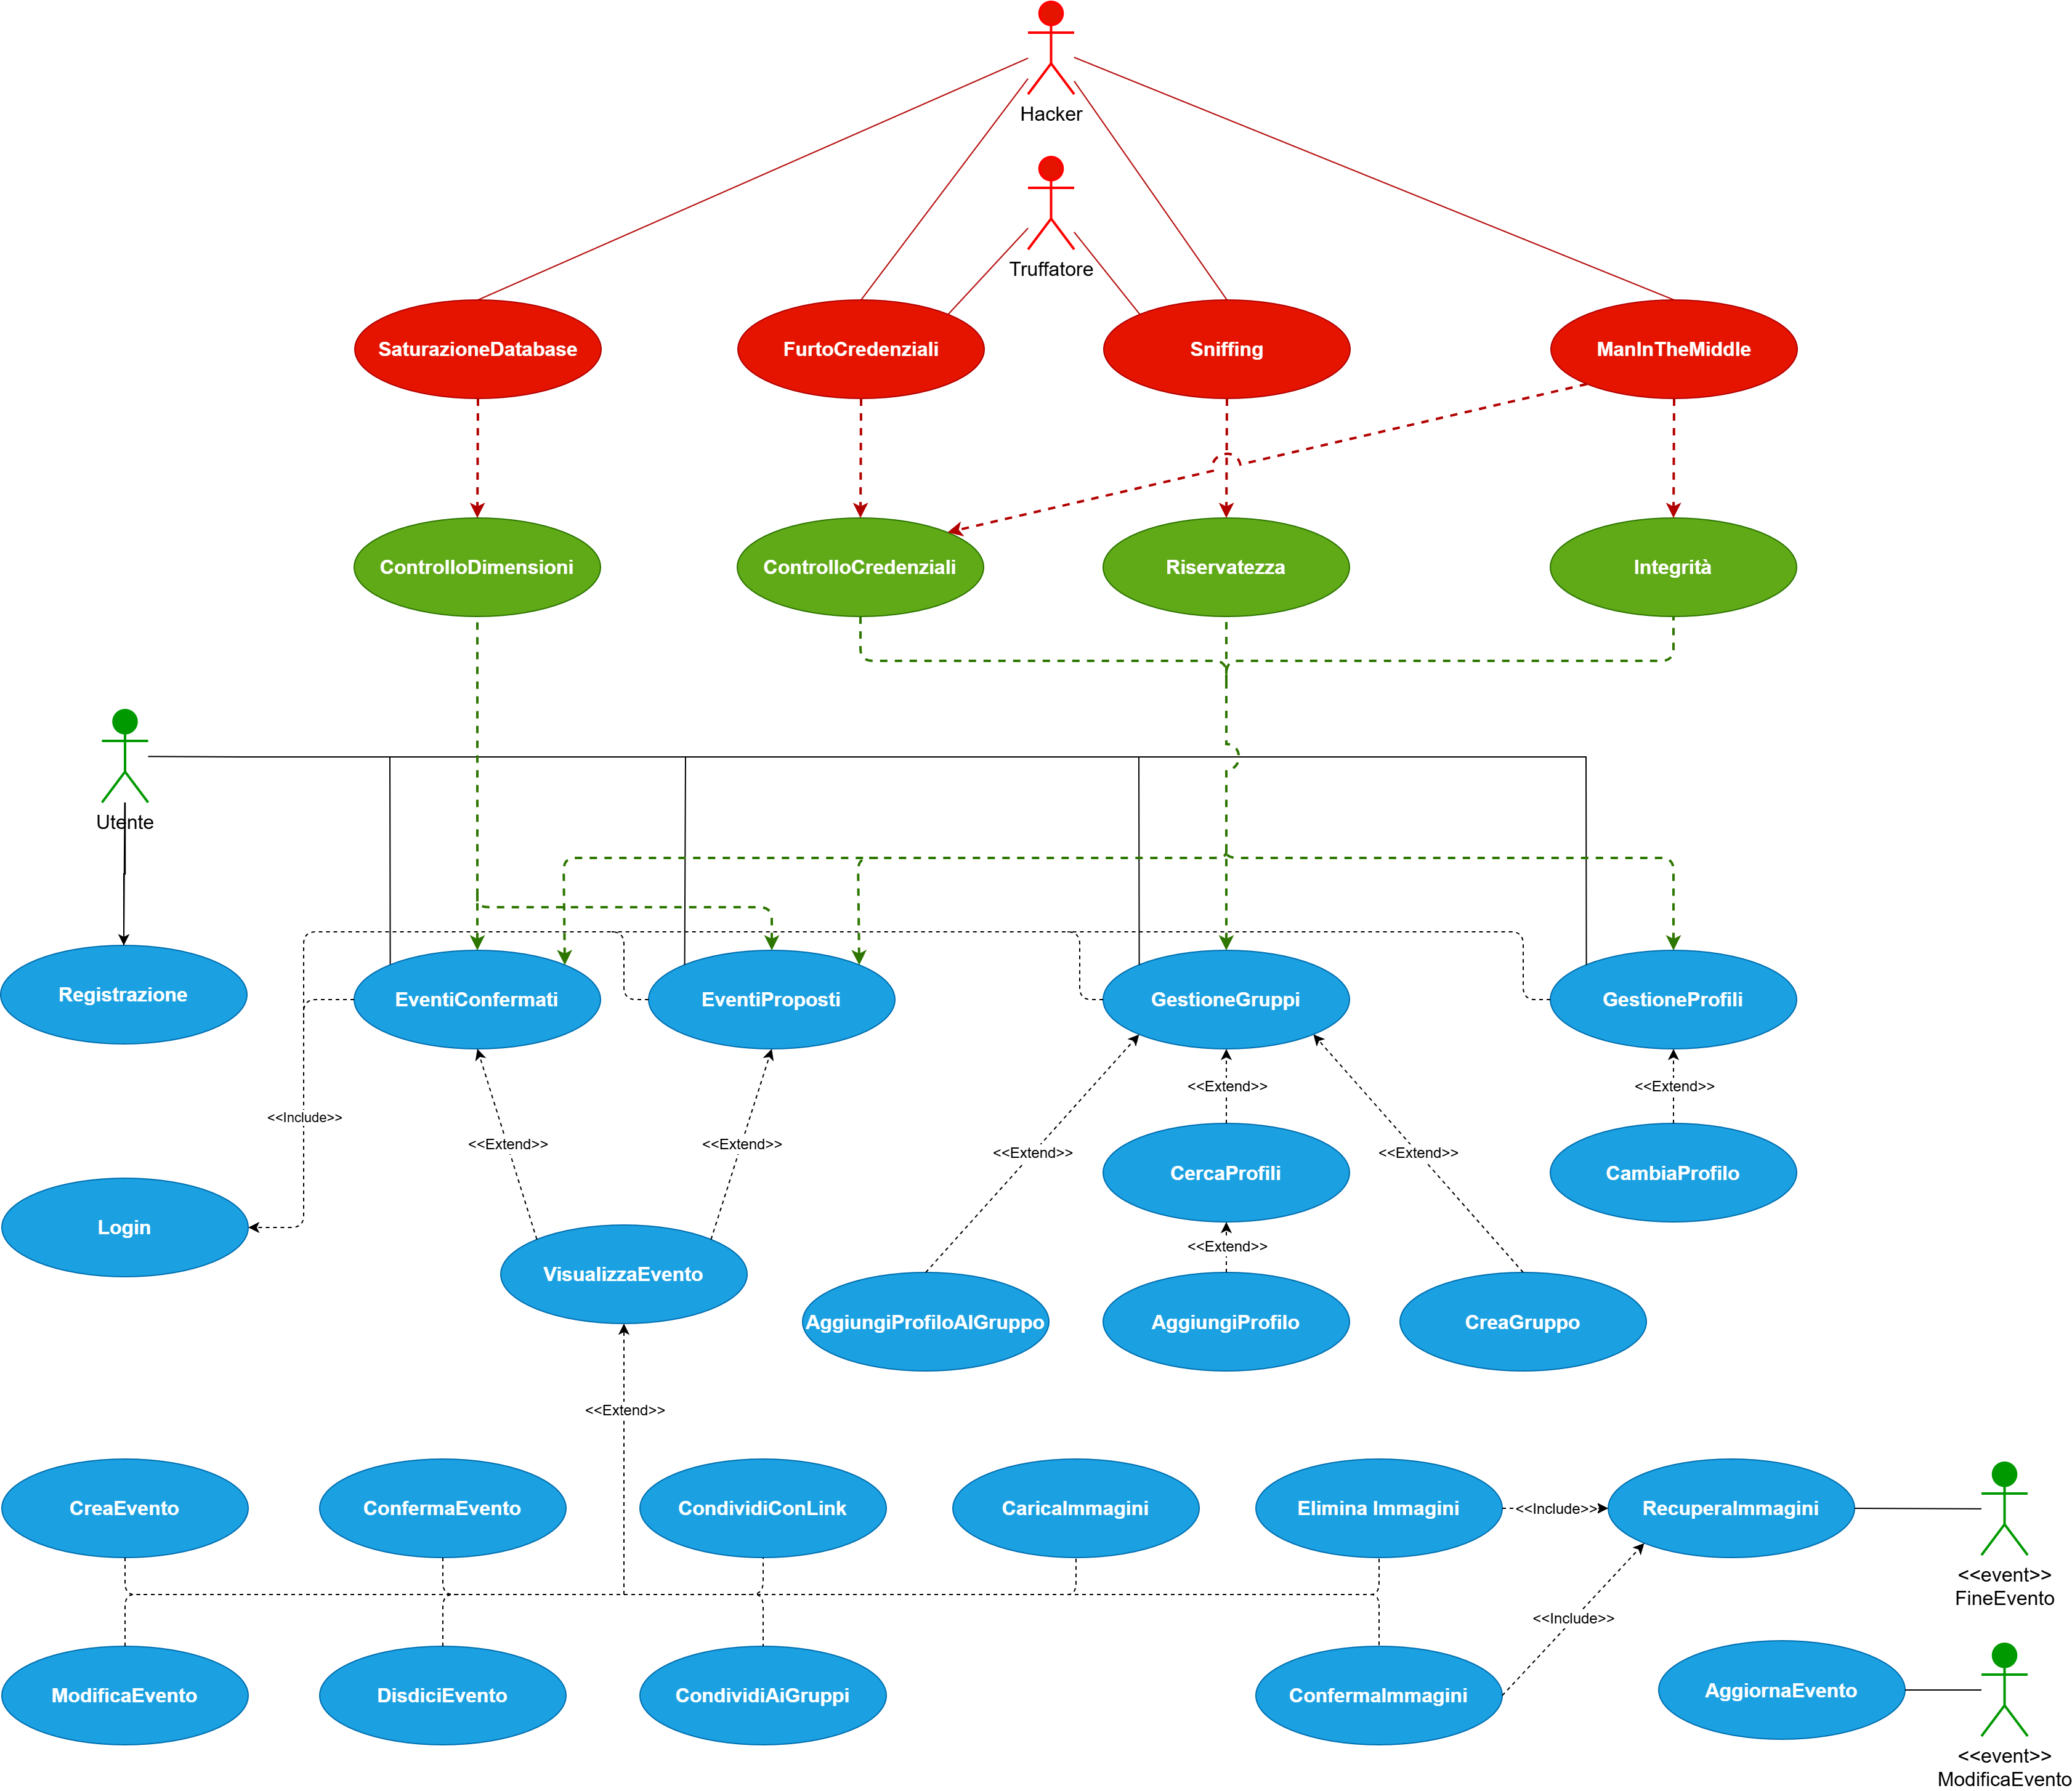
\includegraphics[height=0.6\textheight]{SecurityCase.png}
        \caption{Casi d'uso relativi alla sicurezza}
    \end{center}
\end{figure}
\clearpage

La confidenzialità e l'integrità dei dati sono minacciati dal furto di credenziali,
che permetterebbe a un utente d'identificarsi come qualcun altro;
lo sniffing mina la riservatezza delle comunicazioni, se vengono intercettate;
infine tramite man in the middle un attore malevolo ha la possibilità di modificare le richieste
ingannando entrambi i lati della conversazione.
Si introducono i casi d'uso relativi al controllo delle credenziali,
che aumenta la difficoltà di un possibile furto;
la riservatezza, che permette di nascondere le comunicazioni alle parti non interessate,
e l'integrità, che consente l'individuazione di eventuale manipolazione dei messaggi.\\
\\
Visti i costi e appurate le risorse a disposizione sono stati quindi identificati i seguenti requisiti
inerenti alla protezione dei dati e delle funzionalità di Wyd:

\begin{enumerate}
    \item Implementare un sistema di log per tracciare tutti i messaggi tra i client e i server, inclusi gli accessi, le richieste di prenotazione, di conferma, di sospensione e di invio e ricezione di dati
    \item I dati salvati devono essere protetti da un attaccante che abbia accesso al sistema, prendendo misure di sicurezza fisica, eventualmente cifrando i dati
    \item I dati inviati tra le parti remote devono essere protetti, utilizzando la cifratura dei dati
    \item Tutte le azioni avvenute sul sistema devono essere tracciate tramite un sistema di log.
    \item Il sistema deve essere resistente a un alto numero di richieste contemporanee
    \item La dimensione delle richieste non deve superare una determinata soglia
\end{enumerate}

La visione e l'analisi dei log verrà gestita con uno strumento esterno,
accessibile solo al personale autorizzato.


\begin{longtable}{|P{1.3cm}|P{11.2cm}|P{3cm}|}
    \hline
    \textbf{ID}             & \textbf{Requisiti}                                                                           & \textbf{Tipo}  \\
    \hline
    \endhead
    R21F                    & Implementazione di un sistema di log per tracciare tutti i messaggi
    tra i client e i server & Funzionale                                                                                                    \\
    \hline
    R22F                    & Le richieste non devono superare una certa dimensione                                        & Funzionale     \\
    \hline
    R7NF                    & I dati salvati devono essere protetti da un attaccante che abbia
    accesso al sistema, prendendo misure di sicurezza fisica, eventualmente
    cifrando i dati         & Non Funzionale                                                                                                \\
    \hline
    R8NF                    & I dati inviati tra le parti remote devono essere protetti, utilizzando la cifratura dei dati & Non Funzionale \\
    \hline
    R9NF                    & Il sistema deve essere resistente ad un alto numero di richieste contemporanee               & Non funzionale \\
    \hline
    \caption{Requisiti di sicurezza}
\end{longtable}

\clearpage
%\section{Analisi del problema}

A seguito dell'identificazione dei requisiti e dei casi d'uso,
l'analisi del problema entra nel merito del comportamento dell'applicazione,
evidenziandone il rapporto con le funzionalità.
Determina quindi l'architettura logica, che delinea le relazioni fondamentali del sistema,
individuando i componenti logici principali e le loro responsabilità.\\

\subsection{Analisi delle funzionalità}

Le funzionalità vengono dedotte dai casi d'uso,
sintetizzando i servizi principali dell'applicazione.
In particolare, le funzionalità vengono rilevate in base alla loro relazione con i casi d'uso,
alla specificità del compito che assolvono e alla pertinenza reciproca.\\
\\
Si riportano in tabella le funzionalità che racchiudono altri casi d'uso.\\
In particolare, VisualizzaEvento permette di accedere alla maggior parte delle azioni
che l'utente può attuare sugli eventi.
Allo stesso modo GestioneGruppi e GestioneProfili
permettono di eseguire le azioni correlate al loro contesto.\\

\begin{longtable} {|P{7.3cm}|P{8cm}|}
    \hline
    \textbf{Funzionalità} & \textbf{Scomposizione}                                                                                                                            \\
    \hline
    \endhead
    EventiConfermati      & VisualizzaEvento                                                                                                                                  \\
    \hline
    EventiProposti        & VisualizzaEvento                                                                                                                                  \\
    \hline
    VisualizzaEvento      & CreaEvento, ModificaEvento, ConfermaEvento, DisdiciEvento, CondividiConLink, CondividiAiGruppi, CaricaImmagini, EliminaImmagini, ConfermaImmagini \\
    \hline
    GestioneGruppi        & CercaProfili, AggiungiProfiloAlGruppo, CreaGruppo                                                                                                 \\
    \hline
    CercaProfili          & AggiungiProfilo                                                                                                                                   \\
    \hline
    GestioneProfili       & CambiaProfilo                                                                                                                                     \\
    \hline
    \caption{Scomposizione delle funzionalità}
\end{longtable}

\clearpage

Di ogni funzionalità vengono evidenziati il grado di complessità,
la tipologia di azione che svolgono e i requisiti collegati.
Il grado di complessità riassume la quantità e la difficoltà implementativa
delle azioni che una funzionalità ricopre.
La tipologia riporta in maniera generale la qualità dei servizi offerti.
Infine si riportano gli identificatori dei requisiti funzionali che ogni funzionalità soddisfa.\\
\\
A parte il Login, la Registrazione e  ScritturaLog,
il cui servizio è diretto e uniforme in tutta l'applicazione,
tutte le altre funzionalità prevedono una gestione e manipolazione di più dati,
a volte in strutture complicate,
a volte permettendo una modifica puntuale delle informazioni interessate.


\begin{longtable}{|P{3.8cm}|P{4.5cm}|P{2.5cm}|P{4cm}|}
    \hline
    \textbf{Funzionalità} & \textbf{Tipo}                                                 & \textbf{Grado di complessità} & \textbf{Requisiti Collegati}                    \\
    \hline
    Login                 & Interazione esterno e lettura dati                            & semplice                      & R2F                                             \\
    \hline
    Registrazione         & Interazione esterno e memorizzazione dati                     & semplice                      & R1F                                             \\
    \hline
    EventiConfermati      & Interazione esterno e gestione dati                           & complessa                     & R3F, R8F                                        \\
    \hline
    EventiProposti        & Interazione esterno e gestione dati                           & complessa                     & R4F, R9F                                        \\
    \hline
    GestioneGruppi        & Interazione esterno e gestione dati                           & complessa                     & R15F, R16F                                      \\
    \hline
    GestioneProfili       & Interazione esterno e gestione dati                           & complessa                     & R17F, R18F, R19F                                \\
    \hline
    VisualizzaEvento      & Interazione esterno e gestione, lettura e memorizzazione dati & complessa                     & R5F, R6F, R7F, R8F, R9F, R10F, R11F, R12F, R14F \\
    \hline
    AggiornaEvento        & Gestione dati                                                 & complessa                     & R20F                                            \\
    \hline
    RecuperaImmagini      & Lettura dati                                                  & complessa                     & R13F                                            \\
    \hline
    ScritturaLog          & Memorizzazione dati                                           & semplice                      & R21F                                            \\
    \hline
    \caption{Funzionalità}
\end{longtable}

Si procede analizzando i dati che ogni funzionalità gestisce,
indicandone la tipologia, la protezione richiesta e i vincoli correlati,
per conoscere in maniera definitiva tutte le caratteristiche delle informazioni scambiate.
L'analisi delle informazioni non viene riportata in quanto poco rilevante ai fini della tesi,
ma eventuali dettagli saranno riportati quando necessario.\\
\\
A seguito dell'analisi delle informazioni, si procede con l'analisi dei vincoli,
in cui si chiarificano i requisiti non funzionali,
evidenziandone le criticità e quali componenti ne vengono coinvolti.\\


\begin{longtable} {|P{3.5cm}|P{2cm}|P{3.5cm}|P{6cm}|}
    \hline
    \textbf{Requisito}                  & \textbf{Categorie} & \textbf{Impatto}                                                         & \textbf{Funzionalità}                                                                                                                       \\
    \hline
    \endhead
    Semplicità dell'interfaccia         & Usabilità          & Intuitività di utilizzo                                                  & Login, Registrazione, EventiConfermati, EventiProposti, GestioneGruppi, GestioneProfili, VisualizzaEvento, RecuperaImmagini                 \\
    \hline
    Velocità della ricerca dei dati     & Tempo di Risposta  & Maggiore reattività                                                      & EventiConfermati, EventiProposti, GestioneGruppi, GestioneProfili, RecuperaImmagini                                                         \\
    \hline
    Velocità di memorizzazione dei dati & Tempo di Risposta  & Maggiore reattività                                                      & Registrazione, AggiornaEvento, RecuperaImmagini                                                                                             \\
    \hline
    Controllo Accessi                   & Sicurezza          & Peggiorano tempo di risposta e usabilità, migliorano la privacy dei dati & EventiConfermati, EventiProposti, GestioneGruppi, GestioneProfili, VisualizzaEvento                                                         \\
    \hline
    Protezione dei\linebreak Dati       & Sicurezza          & Peggiorano tempo di risposta, migliorano la privacy dei dati             & Login, Registrazione, EventiConfermati, EventiProposti, GestioneGruppi, GestioneProfili, VisualizzaEvento, AggiornaEvento, RecuperaImmagini \\
    \hline
    Scalabilità delle richieste         & Tempo di Risposta  & Minor degradamento delle prestazioni                                     & EventiConfermati, EventiProposti, AggiornaEvento, RecuperaImmagini                                                                          \\
    \hline
    \caption{Analisi dei vincoli}
\end{longtable}


Infine si definiscono logicamente le maschere,
ovvero i componenti visuali essenziali del programma.
A ogni maschera corrisponderà un'interfaccia grafica
attraverso la quale l'utente potrà accedere alle funzionalità.
Vengono quindi associate le maschere alle funzionalità di cui permettono l'esecuzione,
indicando le informazioni relative.\\
\\

\begin{longtable} {|P{4.5cm}|P{6.5cm}|P{4cm}|}
    \hline
    \textbf{Maschera}     & \textbf{Informazioni}                                                                                                               & \textbf{Funzionalità}                     \\
    \hline
    \endhead
    View Login            & email, password                                                                                                                     & Login                                     \\
    \hline
    View Registrazione    & email, password                                                                                                                     & Registrazione                             \\
    \hline
    View EventiConfermati & lista eventi confermati                                                                                                             & EventiConfermati, AggiornaEvento          \\
    \hline
    View EventiProposti   & lista eventi proposti                                                                                                               & EventiProposti, \linebreak AggiornaEvento \\
    \hline
    View VisualizzaEvento & Identificativo utente, titolo, descrizione, data e orario di inizio, data e orario di fine, confermato, immagini, profili associati & VisualizzaEvento, RecuperaImmagini        \\
    \hline
    View GestioneGruppi   & lista gruppi                                                                                                                        & GestioneGruppi                            \\
    \hline
    View CercaProfili     & tag di ricerca, lista profili                                                                                                       & CercaProfili                              \\
    \hline
    View GestioneProfili  & Lista profili, Identificativo utente, Identificativo profilo corrente                                                               & GestioneProfili                           \\
    \hline
    \caption{Maschere}
\end{longtable}

\clearpage




\subsection{Ideazione dell'architettura logica}
Definite le relazioni e le informazioni relative alle funzionalità,
si esprimono logicamente i componenti principali del sistema e le loro relazioni.
Le funzionalità vengono espresse a livello logico tramite package e diagrammi delle classi,
mentre i dati vengono descritti all'interno del dominio. \\
\\
Il modello del dominio individua le entità che rappresentano logicamente le dipendenze tra i dati.
Ogni entità presenta i suoi dati tramite proprietà,
identificate da un nome e dalla tipologia del dato.
Inoltre, all'interno del modello vengono indicati i rapporti tra le entità specificando le cardinalità reciproche.\\
\\
Il dominio di Wyd si concentra attorno a due entità principali: Event e Profile.\\
Gli Event contengono tutti i dati generali degli eventi,
quali l'ora d'inizio e l'ora di fine, il titolo e la descrizione.
Strettamente correlate a loro ci sono le immagini, identificate con Photo.
Ogni Event può avere più Photo, ma una Photo può essere relativa da un solo Event.
I Profile racchiudono i dati dei profili, 
che devono essere identificati da un Tag unico in tutto il programma.
Group rappresenta un gruppo.
Più Profile possono fare parte di un Group ma, 
allo stesso modo, un Profile può appartenere a più Group.\\
\\
L'Account memorizza le informazioni attraverso cui l'utente può accedere e
agire in quanto User, entità che descrive l'utente.
L'utente ha diverse modalità di accesso,
ed è per questo motivo che più Account possono essere relativi allo stesso User.
Lo stesso utente può impersonare più profili,
e un profilo può essere gestito da più utenti.
User e Profile sono quindi connessi in una relazione molti a molti.\\
\\
La maggior parte delle operazioni avrà a che fare con le due entità principali,
da cui l'importanza dell'elemento che ne descrive la relazione, ovvero ProfileEvent.\\
ProfileEvent ha un ruolo centrale in quanto sarà l'unità interrogata
sia quando si vorranno ottenere gli eventi di un determinato profilo,
sia quando bisognerà recuperare i profili relativi a un evento.
Contiene tutte le informazioni relative al particolare profilo sul determinato evento,
rendendolo infatti l'entità più modificata di tutto il progetto.\\
\\

\begin{figure}[h!]
    \begin{center}
        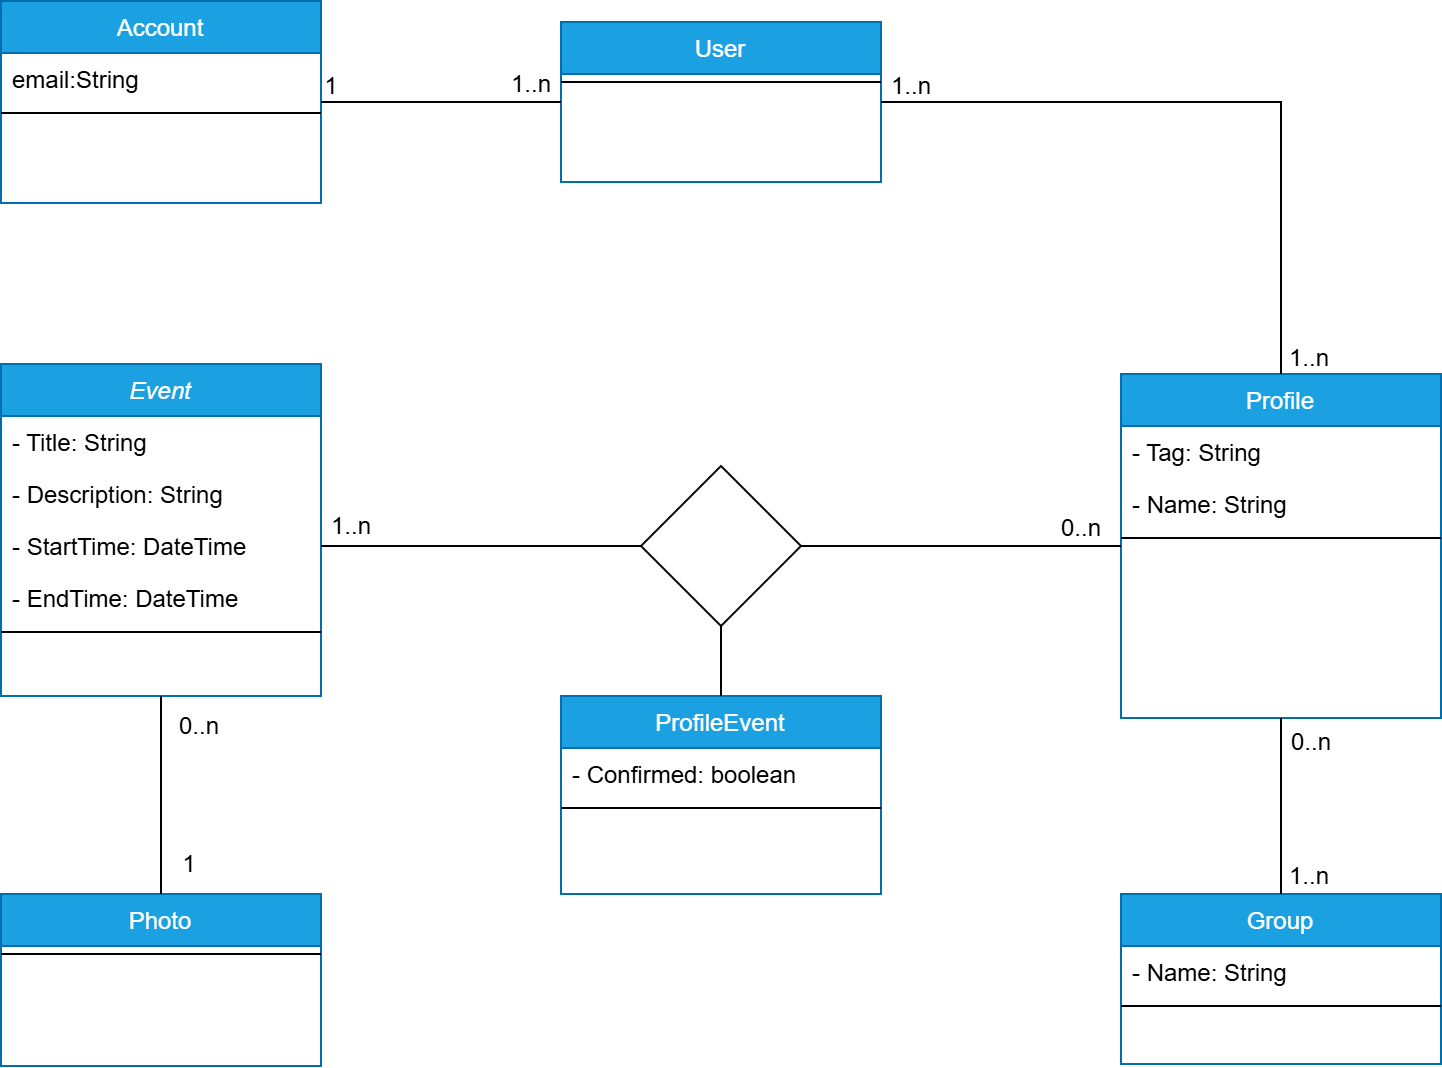
\includegraphics[width=\textwidth]{ModelloDominio.png}
        \caption{Modello del dominio}
    \end{center}
\end{figure}

Il diagramma dei package descrive la divisione delle responsabilità logiche.\\
Ogni package rappresenta una parte di prodotto che soddisfa una determinata responsabilità.
La responsabilità viene individuata in base alla peculiarità e
alle dipendenze delle funzionalità che ricopre.
Si possono così distinguere, ad esempio, package relativi a interfacce grafiche, logiche applicative o gestione della persistenza,
in base alle caratteristiche specifiche del prodotto.
Il diagramma dei package offre una prima struttura delle parti del progetto e del loro rapporto.\\
\\
Distinguiamo i diversi package in base al loro scopo.\\
InterfacciaAccesso e InterfacciaUtente sono le parti che si occuperanno dell'interazione grafica con l'utente.
InterfacciaAccesso deve presentare le schermate di login e di registrazione,
e tutti i passaggi intermedi che saranno necessari.
InterfacciaUtente si occuperà di mostrare le viste per interagire con il resto delle funzionalità dell'applicazione.\\
\\
Il package del Dominio contiene la persistenza principale del progetto,
con tutti i dati delle entità del dominio.
Il package delle Immagini contiene i file multimediali,
recuperabili tramite i metadati salvati sul Dominio.
Il package Log riceve e salva le informazioni relative alle richieste svolte dai vari servizi.\\
\\
GestioneAccesso segue la logica per autenticare gli utenti,
collaborando con InterfacciaAccesso e il Dominio,
per indirizzare l'utente a InterfacciaUtente in caso di login positivo.
GestioneProfilo è il package che racchiude le funzionalità applicative del progetto.
Si occupa quindi d'implementare tutta la logica relativa agli eventi, ai profili e alle loro interazioni.
GestioneAggiornamenti si occupa infine di connettere GestioneProfilo e InterfacciaUtente
per trasmettere le modifiche in tempo reale.\\

\begin{figure}[h!]
    \begin{center}
        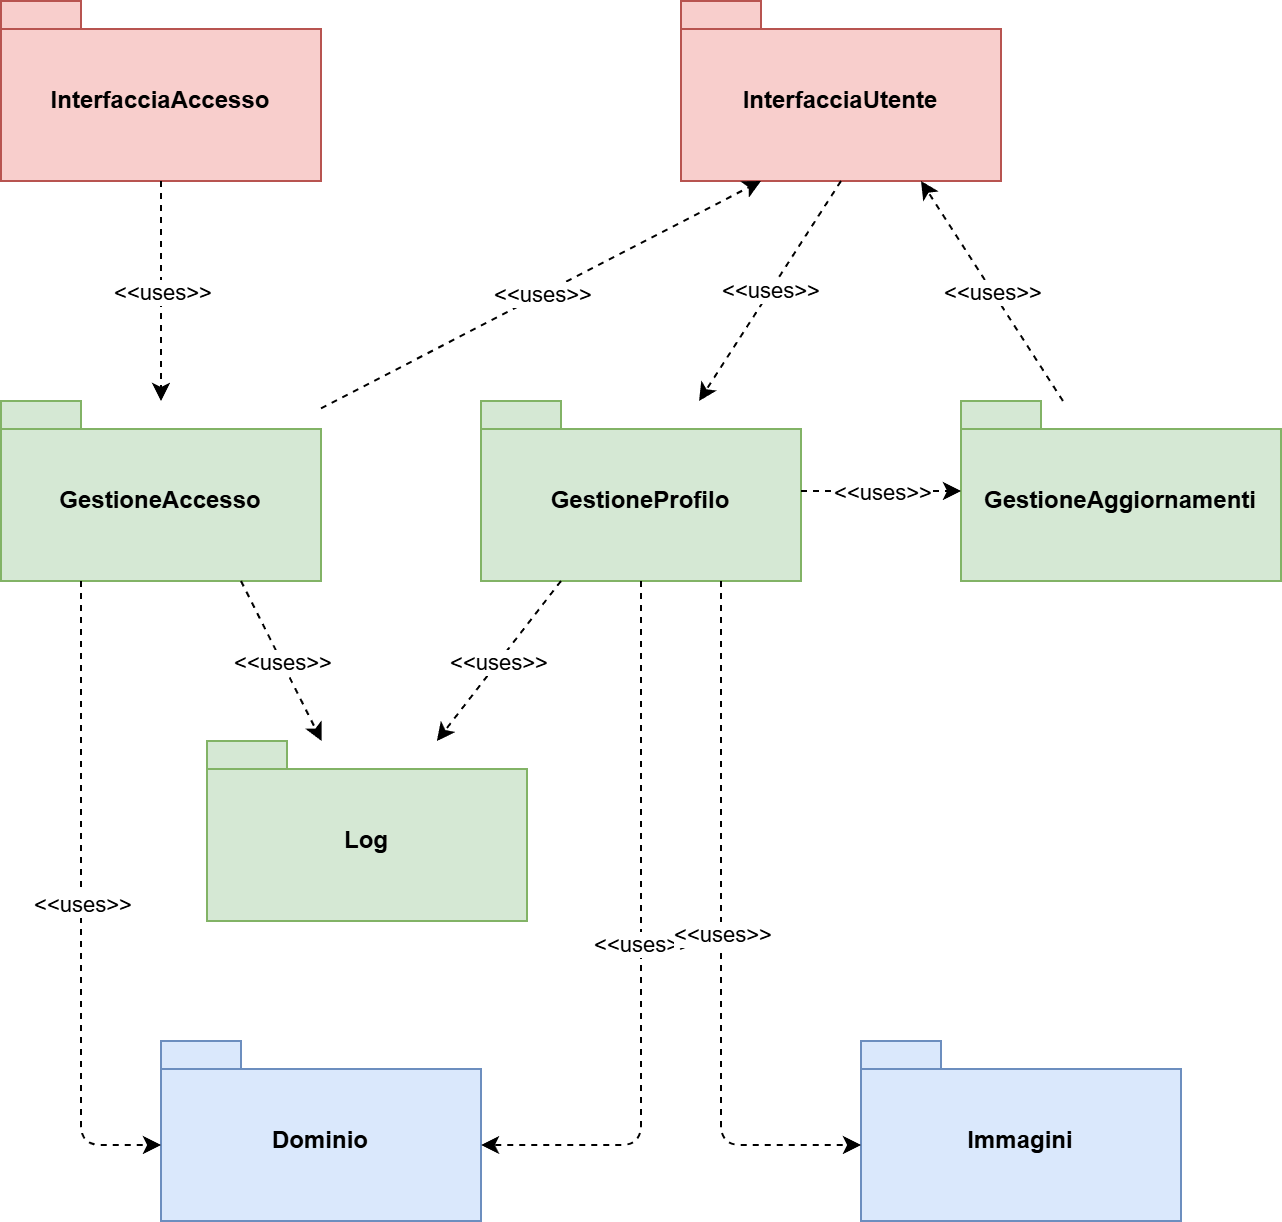
\includegraphics[height=0.5\textheight]{DiagrammaPackage.png}
        \caption{Diagramma dei Package}
    \end{center}
\end{figure}
\clearpage

Ogni package contiene una o più classi che lo implementano.\\
Ogni classe rappresenta un componente logico che assume uno specifico scopo.
Le classi possono presentare dei metodi, ovvero delle istanze che descrivono le funzionalità fornite,
alle quali altri componenti possono fare richiesta di esecuzione.
La definizione delle classi permette di creare una struttura iniziale
presentando le funzionalità minime e le dipendenze tra le parti.\\
\\
InterfacciaUtente ha una classe per ogni funzionalità principale.
Ci sono quindi le classi di ViewEventiConfermati e ViewEventiProposti,
che permettono di visualizzare i relativi impegni.
Attraverso queste interfacce si può interagire con ViewVisualizzaEvento,
per interagire con i dettagli dell'evento.
ViewGestioneGruppi presenta la lista dei gruppi con le azioni relative
e permette l'accesso a ViewCercaProfili,
la schermata per trovare altri profili all'interno dell'applicazione.
ViewGestioneProfili è la classe che visualizza i profili dell'utente e ne permette il cambio.\\

\begin{figure}[h!]
    \begin{center}
        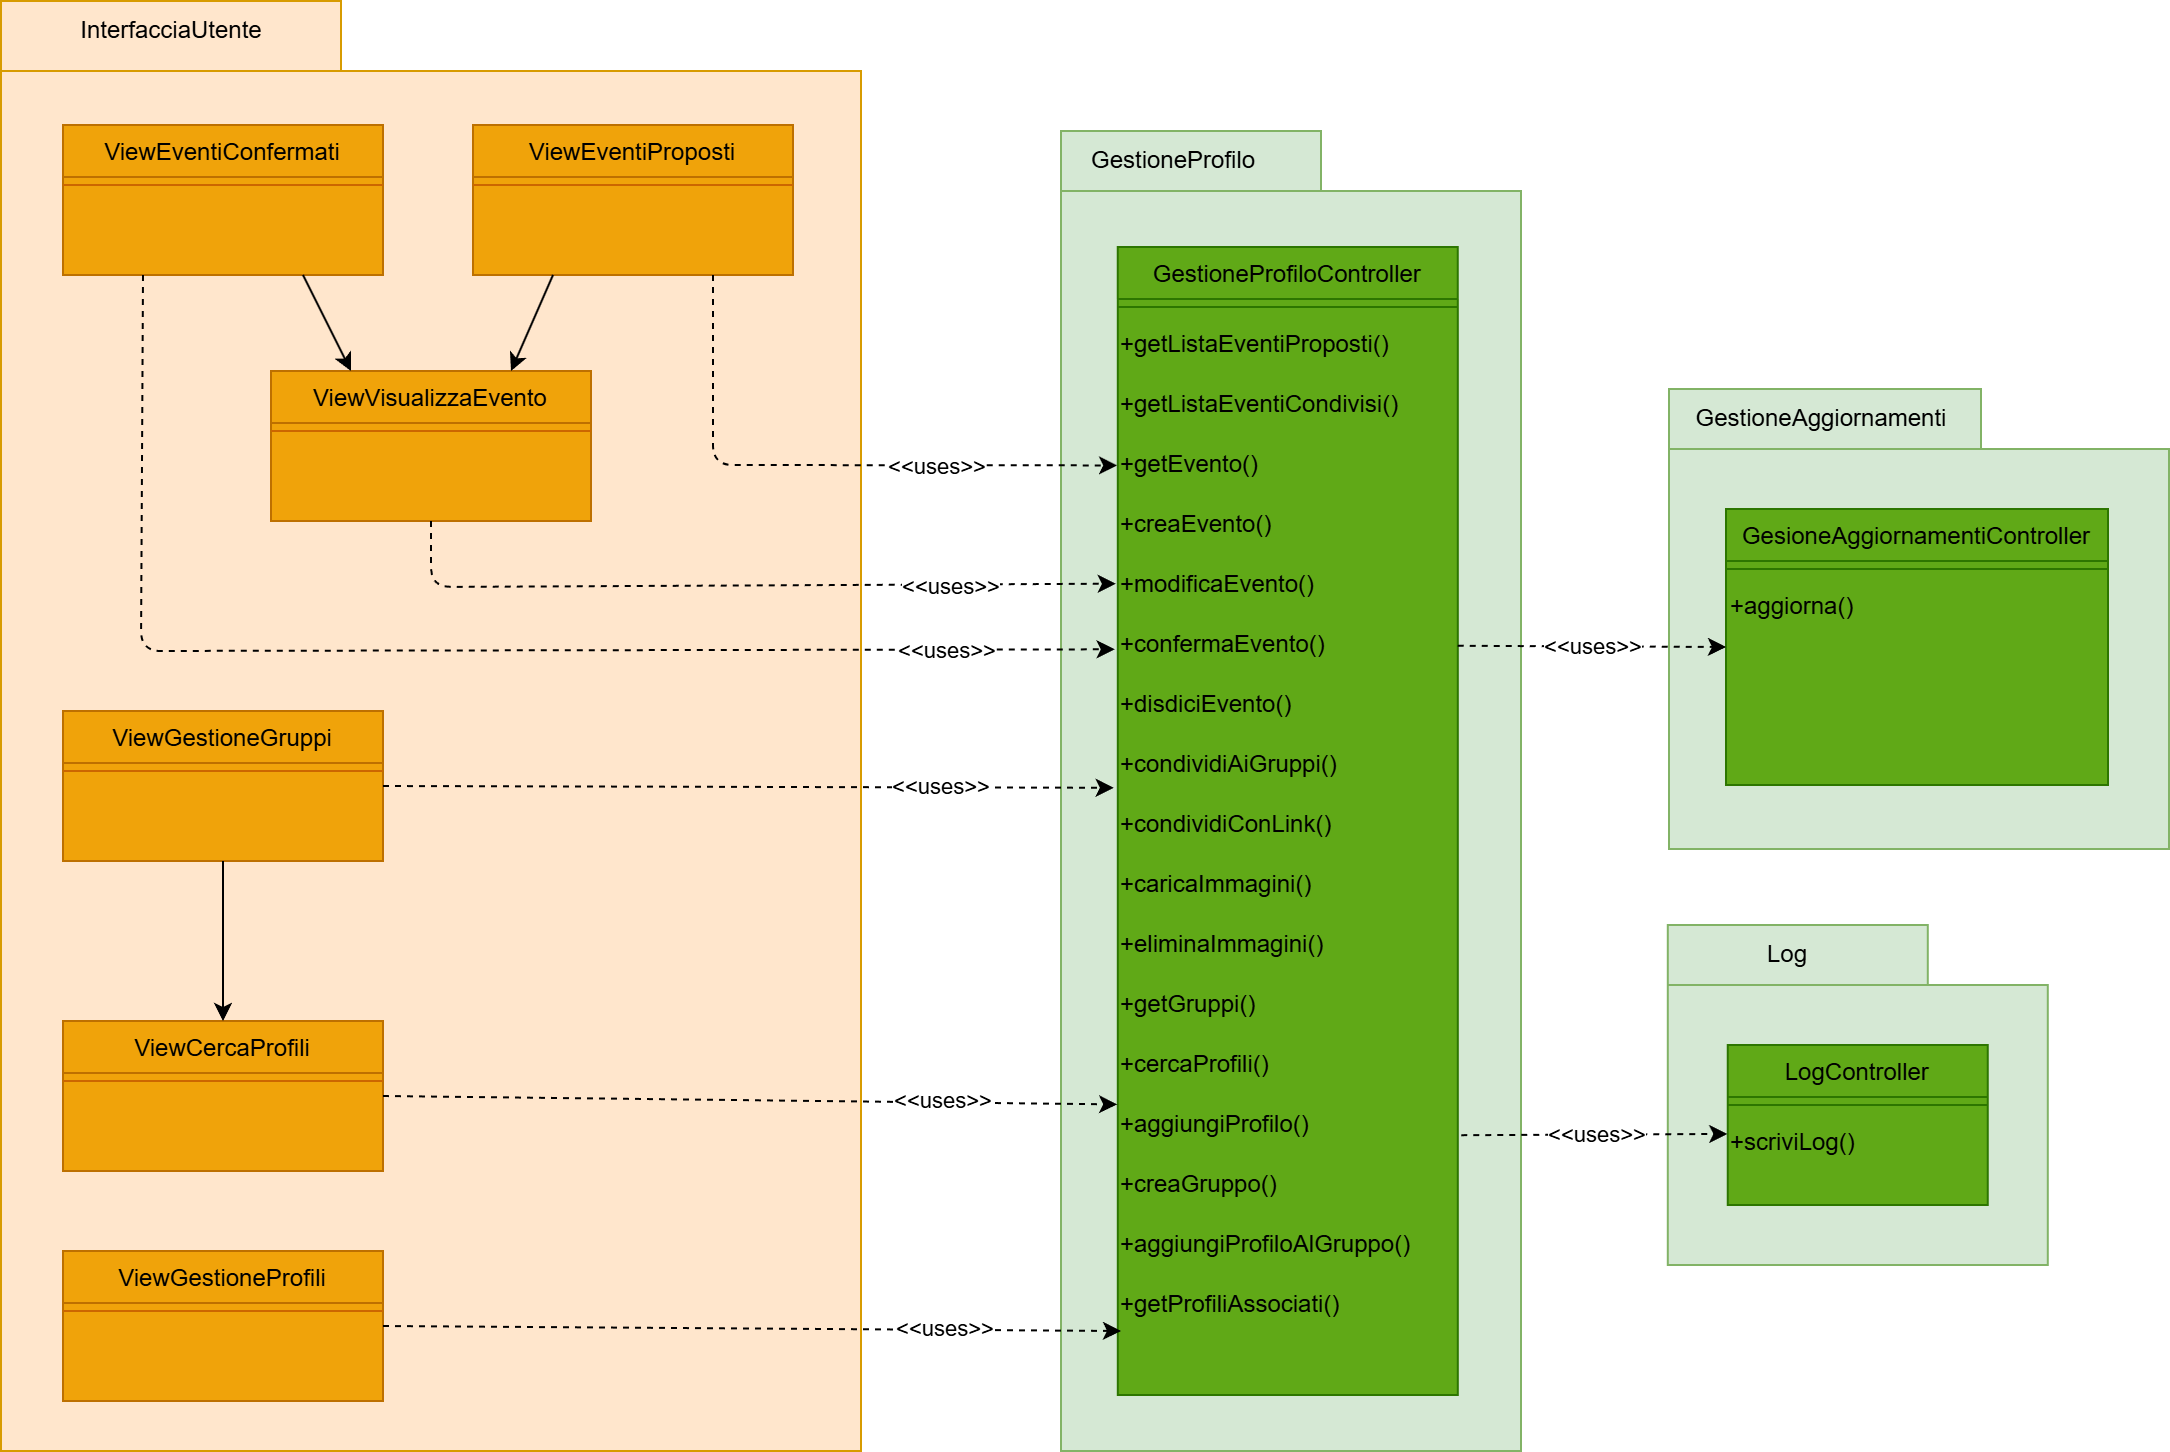
\includegraphics[height=0.46\textheight]{GestioneProfilo.png}
        \caption{Diagramma delle classi: interfaccia utente, gestione profilo e aggiornamenti}
    \end{center}
\end{figure}

GestioneProfilo è il package principale,
a cui le classi di InterfacciaUtente si rivolgono soddisfare le richieste dell'utente.
Prevede una sola classe, GestioneProfiloController,
che risponde alle azioni a cui un profilo può avere accesso, ovvero tutte quelle previste.
Contiene quindi le funzioni relative ai principali casi d'uso,
quali a l'ottenimento degli impegni, la creazione o la conferma dell'evento o il caricamento delle immagini.\\
\\
GestioneAggiornamenti ha il solo compito di aggiornare i dispositivi a seguito di una chiamata da GestioneProfilo,
per cui contiene una classe con un metodo.
InterfacciaAccesso prevede invece due classi, una per il Login e una per la Registrazione.
GestioneAccesso ha una sola classe ma che presenta, seguendo la stessa logica, due metodi distinti.
Il package Log, fornendo un solo metodo, contiene usa sola classe.\\
\\
\begin{figure}[h!]
    \begin{center}
        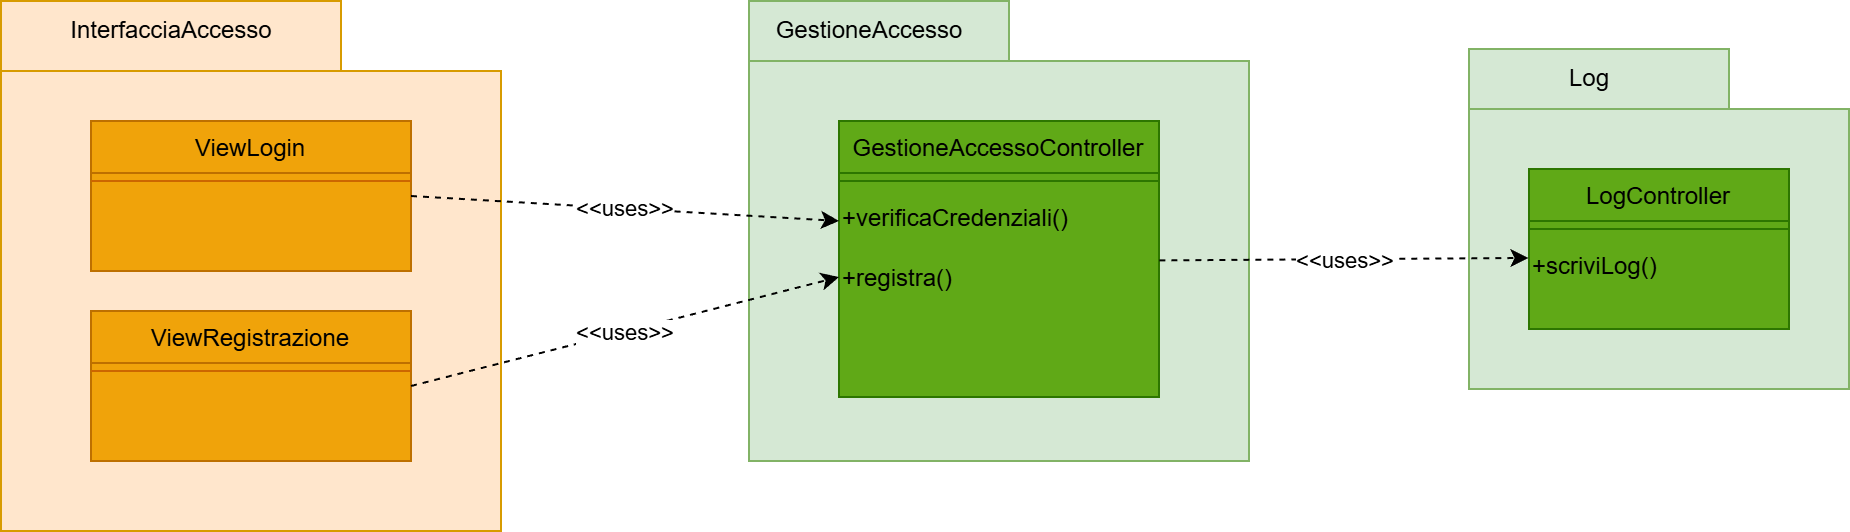
\includegraphics[height=0.18\textheight]{GestioneAccesso.png}
        \caption{Diagramma delle classi: interfacca e gestione accesso}
    \end{center}
\end{figure}



\clearpage
%\chapter{Capitolo 2}

Terminata l'analisi del problema, che ne ha stabilito i requisiti,
le funzionalità e la struttura generale,
si passa alla fase di progettazione.
Durante questa fase l'obiettivo principale è identificare 
le caratteristiche funzionali e comportamentali del sistema,
delineando le componenti principali e le rispettive responsabilità.
Questo permette di definire un'architettura coerente,
facilitando le successive scelte tecnologiche e implementative.\\
\\
Nella fase successiva, di implementazione,
si procede con il passaggio dall'analisi teorica alla realizzazione concreta,
dove la selezione dell'architettura e delle tecnologie di riferimento assumono un ruolo centrale.
Le decisioni prese in questa fase determinano il comportamento dei diversi componenti e
le modalità con cui essi interagiscono tra loro.
Un'attenta selezione delle soluzioni ottimali, 
più adatte ai requisiti definiti in fase di progettazione,
permette di impostare fin dalle prime iterazioni uno sviluppo efficiente e strutturato,
minimizzando la necessità di revisioni successive.\\
\\
Nonostante alcune decisioni risultino immediate o intercambiabili,
altre richiedono analisi approfondite per individuare la soluzione più adatta.
Un approccio efficace consiste nello sviluppare inizialmente i componenti con requisiti ben definiti,
per poi affinare progressivamente l'integrazione e la configurazione con gli altri elementi del sistema.
L'identificazione, anche parziale, di una struttura iniziale 
consente di delineare i vincoli di integrazione e
di semplificare la definizione delle soluzioni mancanti.\\
\\
L'architettura dell'applicativo si basa su una chiara suddivisione in componenti,
ciascuno con un ruolo specifico all'interno del sistema.
\\

Tale organizzazione modulare consente di ottimizzare 
la scalabilità e la manutenibilità dell'applicativo,
facilitando eventuali evoluzioni future.
La suddivisione chiara delle responsabilità, unita a un'architettura flessibile e sicura,
rappresenta quindi un elemento chiave per garantire 
la stabilità e l'efficienza del sistema nel lungo periodo.\\
\\
\begin{figure}[htb]
    \centering
    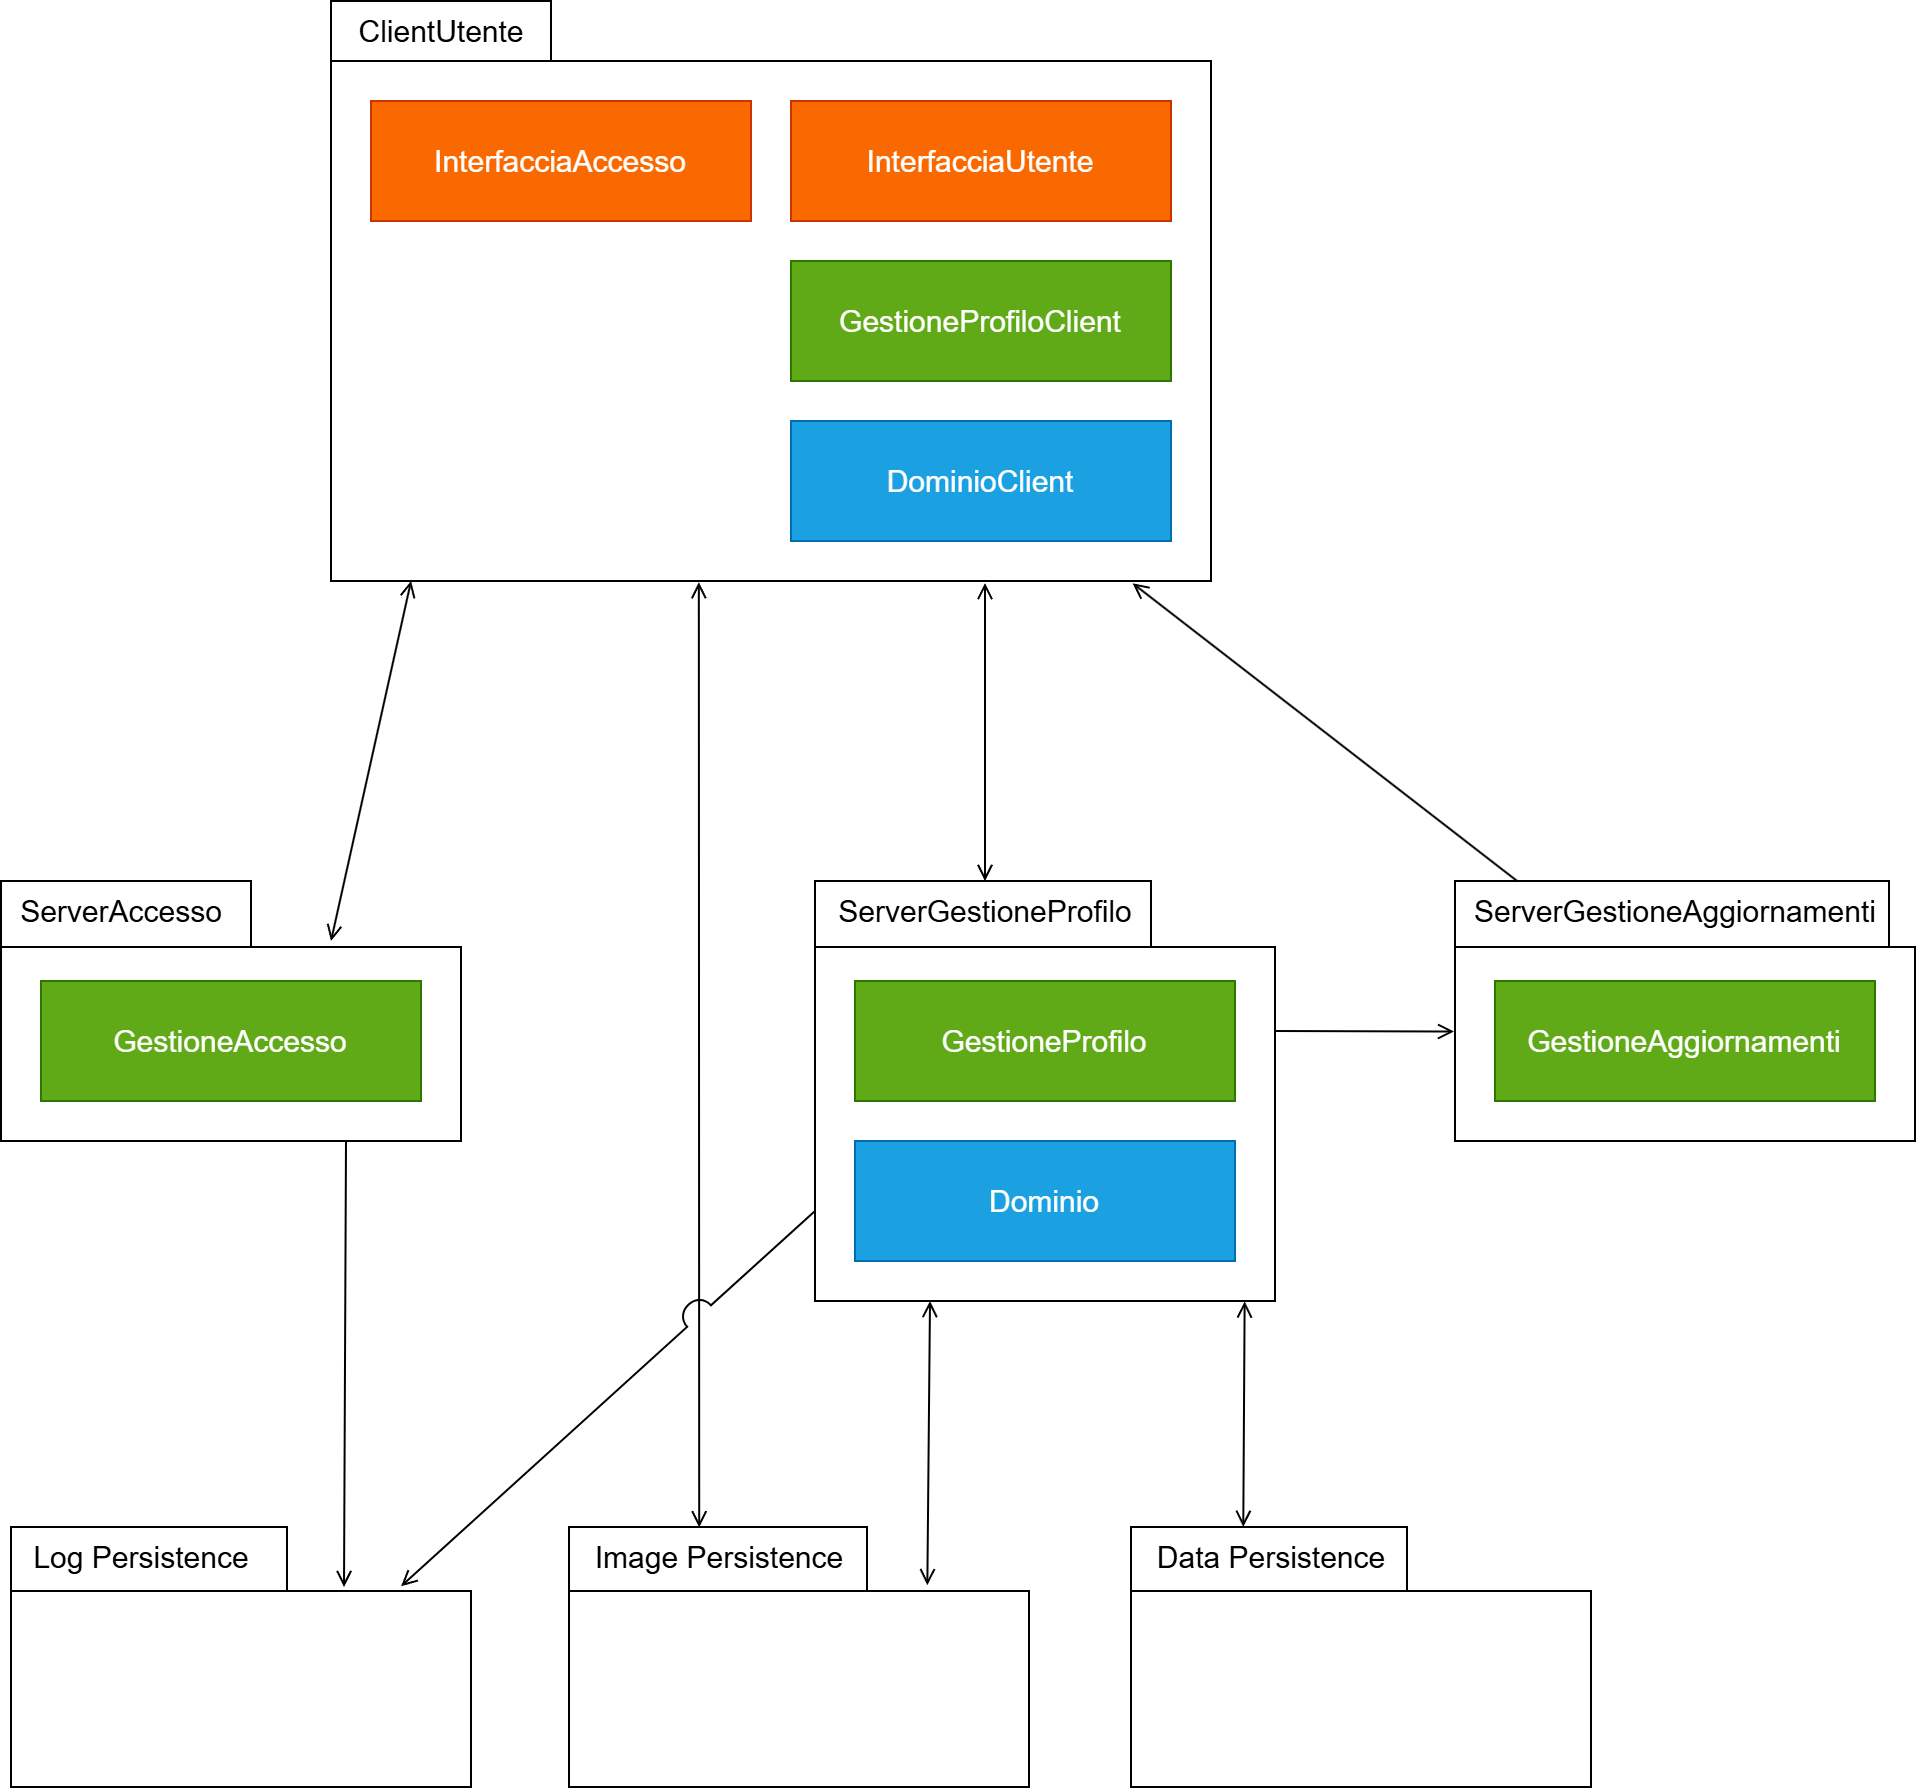
\includegraphics[height=0.67\textheight]{ProgettoDiagrammaPackage.png}
    \caption{Struttura e responsabilità delle parti del progetto}
\end{figure}
\clearpage
L'interfaccia grafica è responsabile della presentazione e dell'interazione con l'utente,
ponendo particolare attenzione alla coerenza visiva e alla fluidità dell'esperienza.
La logica applicativa sarà gestita da un server dedicato,
il quale si occupa di coordinare le comunicazioni tra i diversi servizi
e di garantire il corretto flusso delle operazioni.
La gestione dell'autenticazione degli utenti verrà separata dal resto del sistema,
delegando questa responsabilità a un servizio apposito,
per migliorare sia le prestazioni che la sicurezza.\\
\\
Un ulteriore aspetto fondamentale nella progettazione del sistema riguarda
la protezione delle comunicazioni e dei dati sensibili.
L'adozione di misure di sicurezza adeguate è essenziale
per garantire la protezione delle informazioni scambiate tra i vari componenti e
per ridurre i rischi derivanti da eventuali attacchi esterni.
Inoltre, per monitorare il corretto funzionamento dell'applicazione e
identificare tempestivamente eventuali anomalie,
il sistema è integrato con strumenti di logging e analisi delle prestazioni.\\
\\
\begin{wrapfigure}{o}{0.25\textwidth}
    \centering
    
\includegraphics[height=.12\textheight]{azure.png}
    Azure
\end{wrapfigure}
Già consolidata e affidabile,
sin dalle prime fasi di sviluppo del progetto è stata adottata la piattaforma cloud Azure,
per garantire un'infrastruttura solida e scalabile.
\clearpage
\section{Sviluppo del client utente}
L'utilizzo delle applicazioni per la gestione degli eventi
può essere suddiviso in due fasi distinte,
ciascuna con specifiche esigenze funzionali.\\
\\
La prima fase riguarda la pianificazione a lungo termine e l'organizzazione degli impegni.
In questa circostanza l'utente decide come distribuire il proprio tempo, 
pianificando attività e appuntamenti,
e strutturando il proprio calendario nel modo più efficiente per le proprie necessità.
La seconda fase riguarda invece la gestione degli eventi non ancora certi e definiti;
ciò include l'invito a un evento, l'eventuale conferma da parte dell'utente,
l'identificazione degli impegni a breve termine e l'aggiornamento del loro stato
(ad esempio, se l'evento sia ancora confermato, quante persone vi partecipano,
se qualcuno ha annullato o se l'evento è già concluso)
con la gestione degli eventuali contenuti multimediali successivi all'evento.
Queste due fasi implicano un approccio diverso da parte dell'utente,
comportando di conseguenza esigenze differenti
a cui l'applicazione deve rispondere adeguatamente.\\
\\
Per rispondere a tali necessità, 
è fondamentale che l'applicazione offra un'interfaccia utente versatile,
fruibile sia da desktop che da dispositivi mobili.
La versione desktop consente una pianificazione a lungo termine,
offrendo una visione d'insieme chiara e completa di tutti gli impegni,
tale da facilitare la gestione del tempo.
D'altra parte, la versione mobile deve permettere una gestione rapida e dinamica degli eventi quotidiani,
garantendo che l'utente possa rimanere sempre connesso e aggiornato sugli sviluppi in tempo reale.\\
\\
Inoltre, considerando che l'applicazione è destinata
a un utilizzo diffuso e a un'utenza potenzialmente elevata,
è necessario garantire tempi di risposta ridotti e 
una gestione efficiente delle richieste concorrenti.
Ciò implica la progettazione di un sistema in grado di scalare facilmente,
per supportare un ampio numero di utenti simultanei senza compromettere le prestazioni.
\clearpage
\subsection{Scelta del framework di sviluppo}

Al fine di ottenere tutte le prestazioni precedentemente elencate,
la scelta è ricaduta sull'adozione del framework di sviluppo Flutter.
Diversi fattori motivano tale decisione. \\
\begin{wrapfigure}{o}{0.25\textwidth}
    \centering
    
\includegraphics[height=.12\textheight]{flutter.png}
    Flutter
\end{wrapfigure}
In primo luogo, l'architettura di Flutter si basa su un motore grafico
indipendente dalla piattaforma di esecuzione,
il che consente di semplificare lo sviluppo,
concentrando il codice in un unico progetto ed
evitando quindi di dover implementare una versione diversa
per ogni tecnologia su cui si voglia distribuire l'applicazione.
L'astrazione fornita permette inoltre di ottenere elevate prestazioni e
garantire un'esperienza utente uniforme indipendentemente dal dispositivo usato.
In secondo luogo, Flutter adotta un approccio dichiarativo 
nella progettazione dell'interfaccia grafica,
che facilita lo sviluppo di componenti reattivi attraverso un codice conciso, 
facilmente mantenibile.\\
\\
Un ulteriore vantaggio di Flutter è rappresentato dalla sua crescente adozione nel settore,
dalla solidità della community di sviluppo e dal supporto offerto da Google,
che ne assicurano la stabilità, l'efficienza, la sicurezza e la disponibilità
di componenti personalizzabili per l'intero ciclo di vita del prodotto.
Infine, Flutter consente uno sviluppo rapido e interattivo
grazie alla sua sintassi intuitiva e al meccanismo di hot reload,
che riduce significativamente i tempi di compilazione e facilita il testing in tempo reale.\\
\\
Tra le altre tecnologie valutate per lo sviluppo dell'interfaccia grafica vi erano React Native e Xamarin.
Tuttavia, entrambe presentano alcune limitazioni:
le applicazioni finali sviluppate con React Native tendono ad avere dimensioni più elevate e
le prestazioni risultano inferiori,
in particolare nella gestione della memoria.
Xamarin, pur essendo una valida opzione, presenta una curva di apprendimento più ripida e
una comunità di sviluppatori ridotta rispetto a Flutter,
con una conseguente minore disponibilità di componenti e librerie.\\
\\
L'applicazione utente ha come obiettivo la soddisfazione di due compiti principali:
interagire con l'utente e comunicare con il server,
per recuperare i dati e salvare le modifiche apportate.

\subsection{Realizzazione delle interfacce grafiche}

L'interazione utente avviene tramite interfacce grafiche
che permettono di visualizzare i dati e le funzionalità a disposizione.
Per rispettare il requisito di semplicità e fluidità dell'esperienza è essenziale che
ogni interfaccia sia il più intuitiva possibile,
tramite una limitata varietà di azioni nella stessa pagina.
Ogni azione deve essere facilmente accessibile,
ma anche riconoscibile in base alla sua importanza e funzionalità.\\
\\
Per ogni maschera individuata in fase di analisi
corrisponde almeno un'interfaccia grafica che,
oltre a gestire la navigazione con le altre interfacce,
permette all'utente di eseguire le proprie funzionalità,
esponendo chiaramente le informazioni,
concentrando l'attenzione sui dati eventualmente richiesti
e segnalando le azioni eseguibili.\\
\\
Nei diagrammi di dettaglio le interfacce 
vengono presentate elencando le funzionalità di cui dispongono,
assieme alle loro relazioni di dipendenza.
Si riportano le interfacce di gestione dei gruppi e di visualizzazione degli eventi,
in quanto funzionalità centrali, il cui stile grafico è stato rispettato nella creazione del resto dell'applicazione.\\
\begin{figure}[htbp]
    \begin{center}
        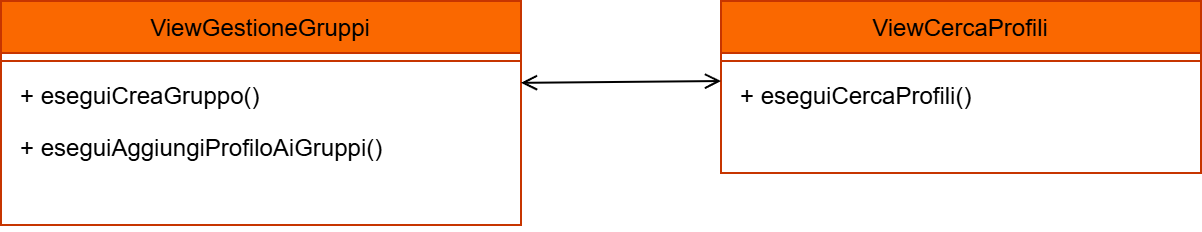
\includegraphics[width=\textwidth]{ProgettoViewGruppi.png}
        \caption{Diagramma di dettaglio delle interfacce di gestione dei gruppi}
    \end{center}
\end{figure}
\\
L'interfaccia della gestione dei gruppi ha il compito di presentare tutti i gruppi
associati al profilo attualmente in uso,
fornendo l'accesso alle azioni relative.
Li elenca quindi in maniera chiara,
definendo la differenza tra gruppi di due o più persone.
Per ognuno mostra un bottone dal quale, se selezionato,
compariranno le azioni attuabili sul gruppo
(ad esempio, di aggiungere un profilo).\\
\\
Correlata alla gestione dei profili c'è la loro ricerca,
che consente il ritrovamento e la successiva aggiunta dei profili tra i propri gruppi.
La schermata risulta minimale,
consentendo all'utente di concentrarsi sulle sole informazioni e funzionalità essenziali.\\

\begin{figure}[htbp]
    \centering
    \begin{subfigure}{0.49\textwidth}
        \centering
        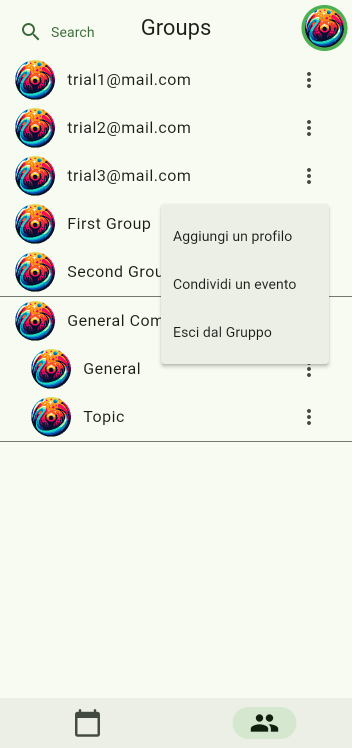
\includegraphics[height=15cm, keepaspectratio]{gruppi.png}
        \caption{Elenco dei gruppi}
    \end{subfigure}
    \hfill
    \begin{subfigure}{0.49\textwidth}
        \centering
        
\includegraphics[height=15cm, keepaspectratio]{cerca.png}
        \caption{Ricerca dei profili}
    \end{subfigure}
    \caption{Schermate dei profili}
\end{figure}

La visualizzazione degli eventi prevede due componenti principali.\\
\\
Il primo consiste in una panoramica generale,
affiancando gli eventi tra loro a livello settimanale,
per fornire all'utente un quadro complessivo degli impegni.
Tale vista è ripetuta sia per gli eventi proposti che per quelli confermati,
con la possibilità di navigare tra le due schermate.\\
\\
Il secondo entra nel particolare dell'evento,
mostrando i dettagli relativi e fornendo la possibilità di modificarli.
Concentra inoltre le principali funzionalità dell'applicazione,
quali la conferma della partecipazione all'evento,
la condivisione con i gruppi e il caricamento delle immagini.\\
\\
\begin{figure}[h!]
    \begin{center}
        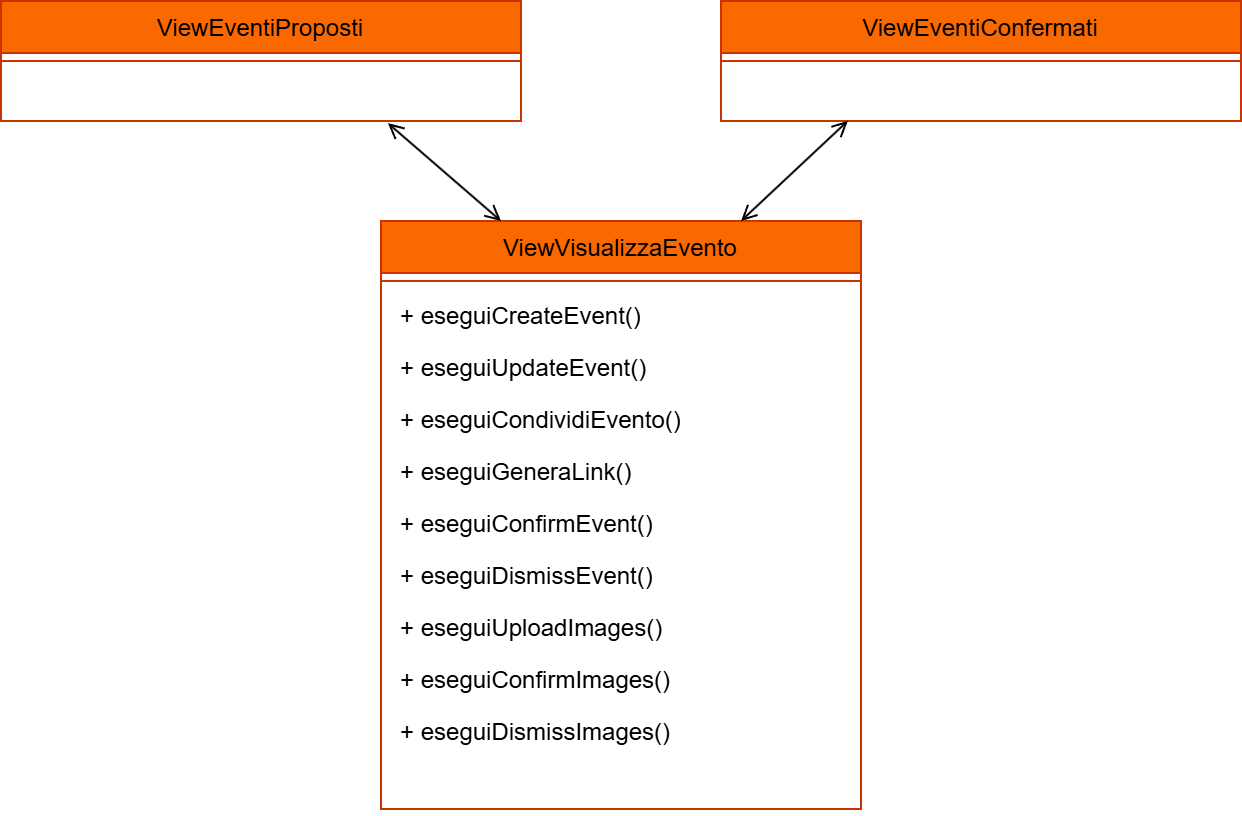
\includegraphics[width=\textwidth]{ProgettoViewEventi.png}
        \caption{Diagramma di dettaglio delle interfacce di visualizzazione eventi}
    \end{center}
\end{figure}

Queste due funzionalità sono al centro del servizio del sistema,
ed è quindi essenziale che l'interfaccia proposta sia veloce ma sopratutto intuitiva.
Fondamentale in questo riguardo è l'importanza data dai colori, attraverso i quali
ogni elemento risalta in base alla sua importanza, e fornisce il suo contesto e le sue proprietà
grazie al puro impatto visivo.\\
\\



\begin{figure}[htbp]
    \centering
    \begin{subfigure}{0.49\textwidth}
        \centering
        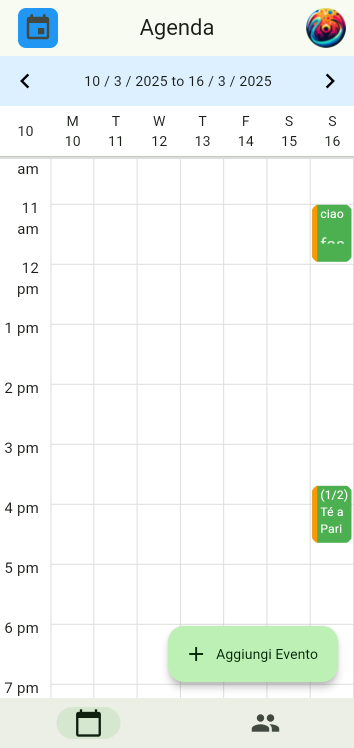
\includegraphics[height=15cm, keepaspectratio]{agenda.png}
        \caption{Visualizzazione generale degli eventi}
    \end{subfigure}
    \hfill
    \begin{subfigure}{0.49\textwidth}
        \centering
        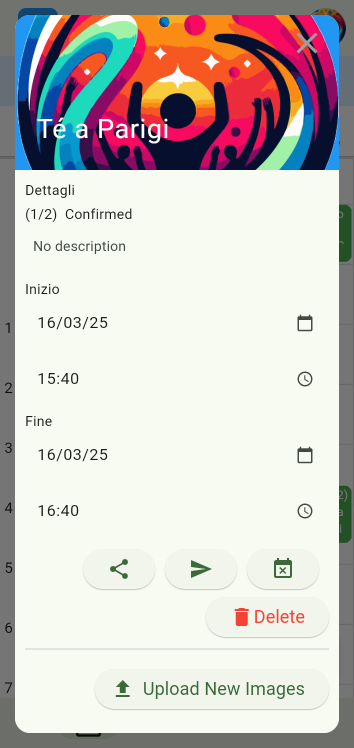
\includegraphics[height=15cm, keepaspectratio]{evento.png}
        \caption{Dettaglio di un evento}
    \end{subfigure}
    \caption{Schermate degli eventi}
\end{figure}

\clearpage

\subsection{Implementazione della logica applicativa}

Ogni interazione con l'utente scatena una qualche forma di elaborazione di dati.
La visualizzazione di qualunque componente comporta la ricerca delle informazioni,
la loro modifica necessita di essere salvata e
la loro condivisione esige la propagazione degli aggiornamenti.
Inoltre, alcuni casi d'uso richiedono azioni da svolgere in autonomia.
L'implementazione della logica necessaria,
per rispondere efficacemente ai requisiti di velocità ed efficienza,
avviene tramite la creazione di diversi componenti.\\
\\
La suddivisione del programma individua e raggruppa le funzionalità in base al loro contesto,
affidando a ogni componente meno responsabilità possibili.
Questo permette di concentrare le logiche condivise,
evitando duplicazioni e definendo chiaramente il ruolo di ogni metodo.
La semplicità del codice così raggiunta semplifica il futuro sviluppo e la sua manutenzione.\\
\\
La principale suddivisione dei componenti avviene in base agli elementi del dominio.
Per ogni principale entità, infatti, viene creato un servizio che ne racchiude
le richieste di ritrovamento, modifica e salvataggio correlate.
Collegando i servizi al dominio si concentrano anche le eventuali dipendenze da altri servizi,
riducendole alle sole inerenti all'elemento specifico,
mantenendo un parallelismo logico anche a livello di relazione.\\
\\
La maggior parte delle richieste 
che riguardano gli elementi del dominio prevede
la comunicazione con il server esterno.
La ricezione e l'aggiornamento dei dati,
così come la permanenza delle modifiche,
avvengono infatti attraverso l'interazione con la persistenza principale, 
a cui si accede tramite il server.
Vista la complessità specifica nella gestione delle trasmissioni e
la loro secondaria importanza a livello logico,
vengono realizzati dei componenti dedicati, chiamati API.
I componenti API hanno il compito di gestire le trasmissioni 
astraendo il rapporto con il server,
semplificando così il codice e separando la logica applicativa 
dalle complessità richieste dalla tecnologia di comunicazione usata.

\clearpage

\begin{figure}[h!]
    \begin{center}
        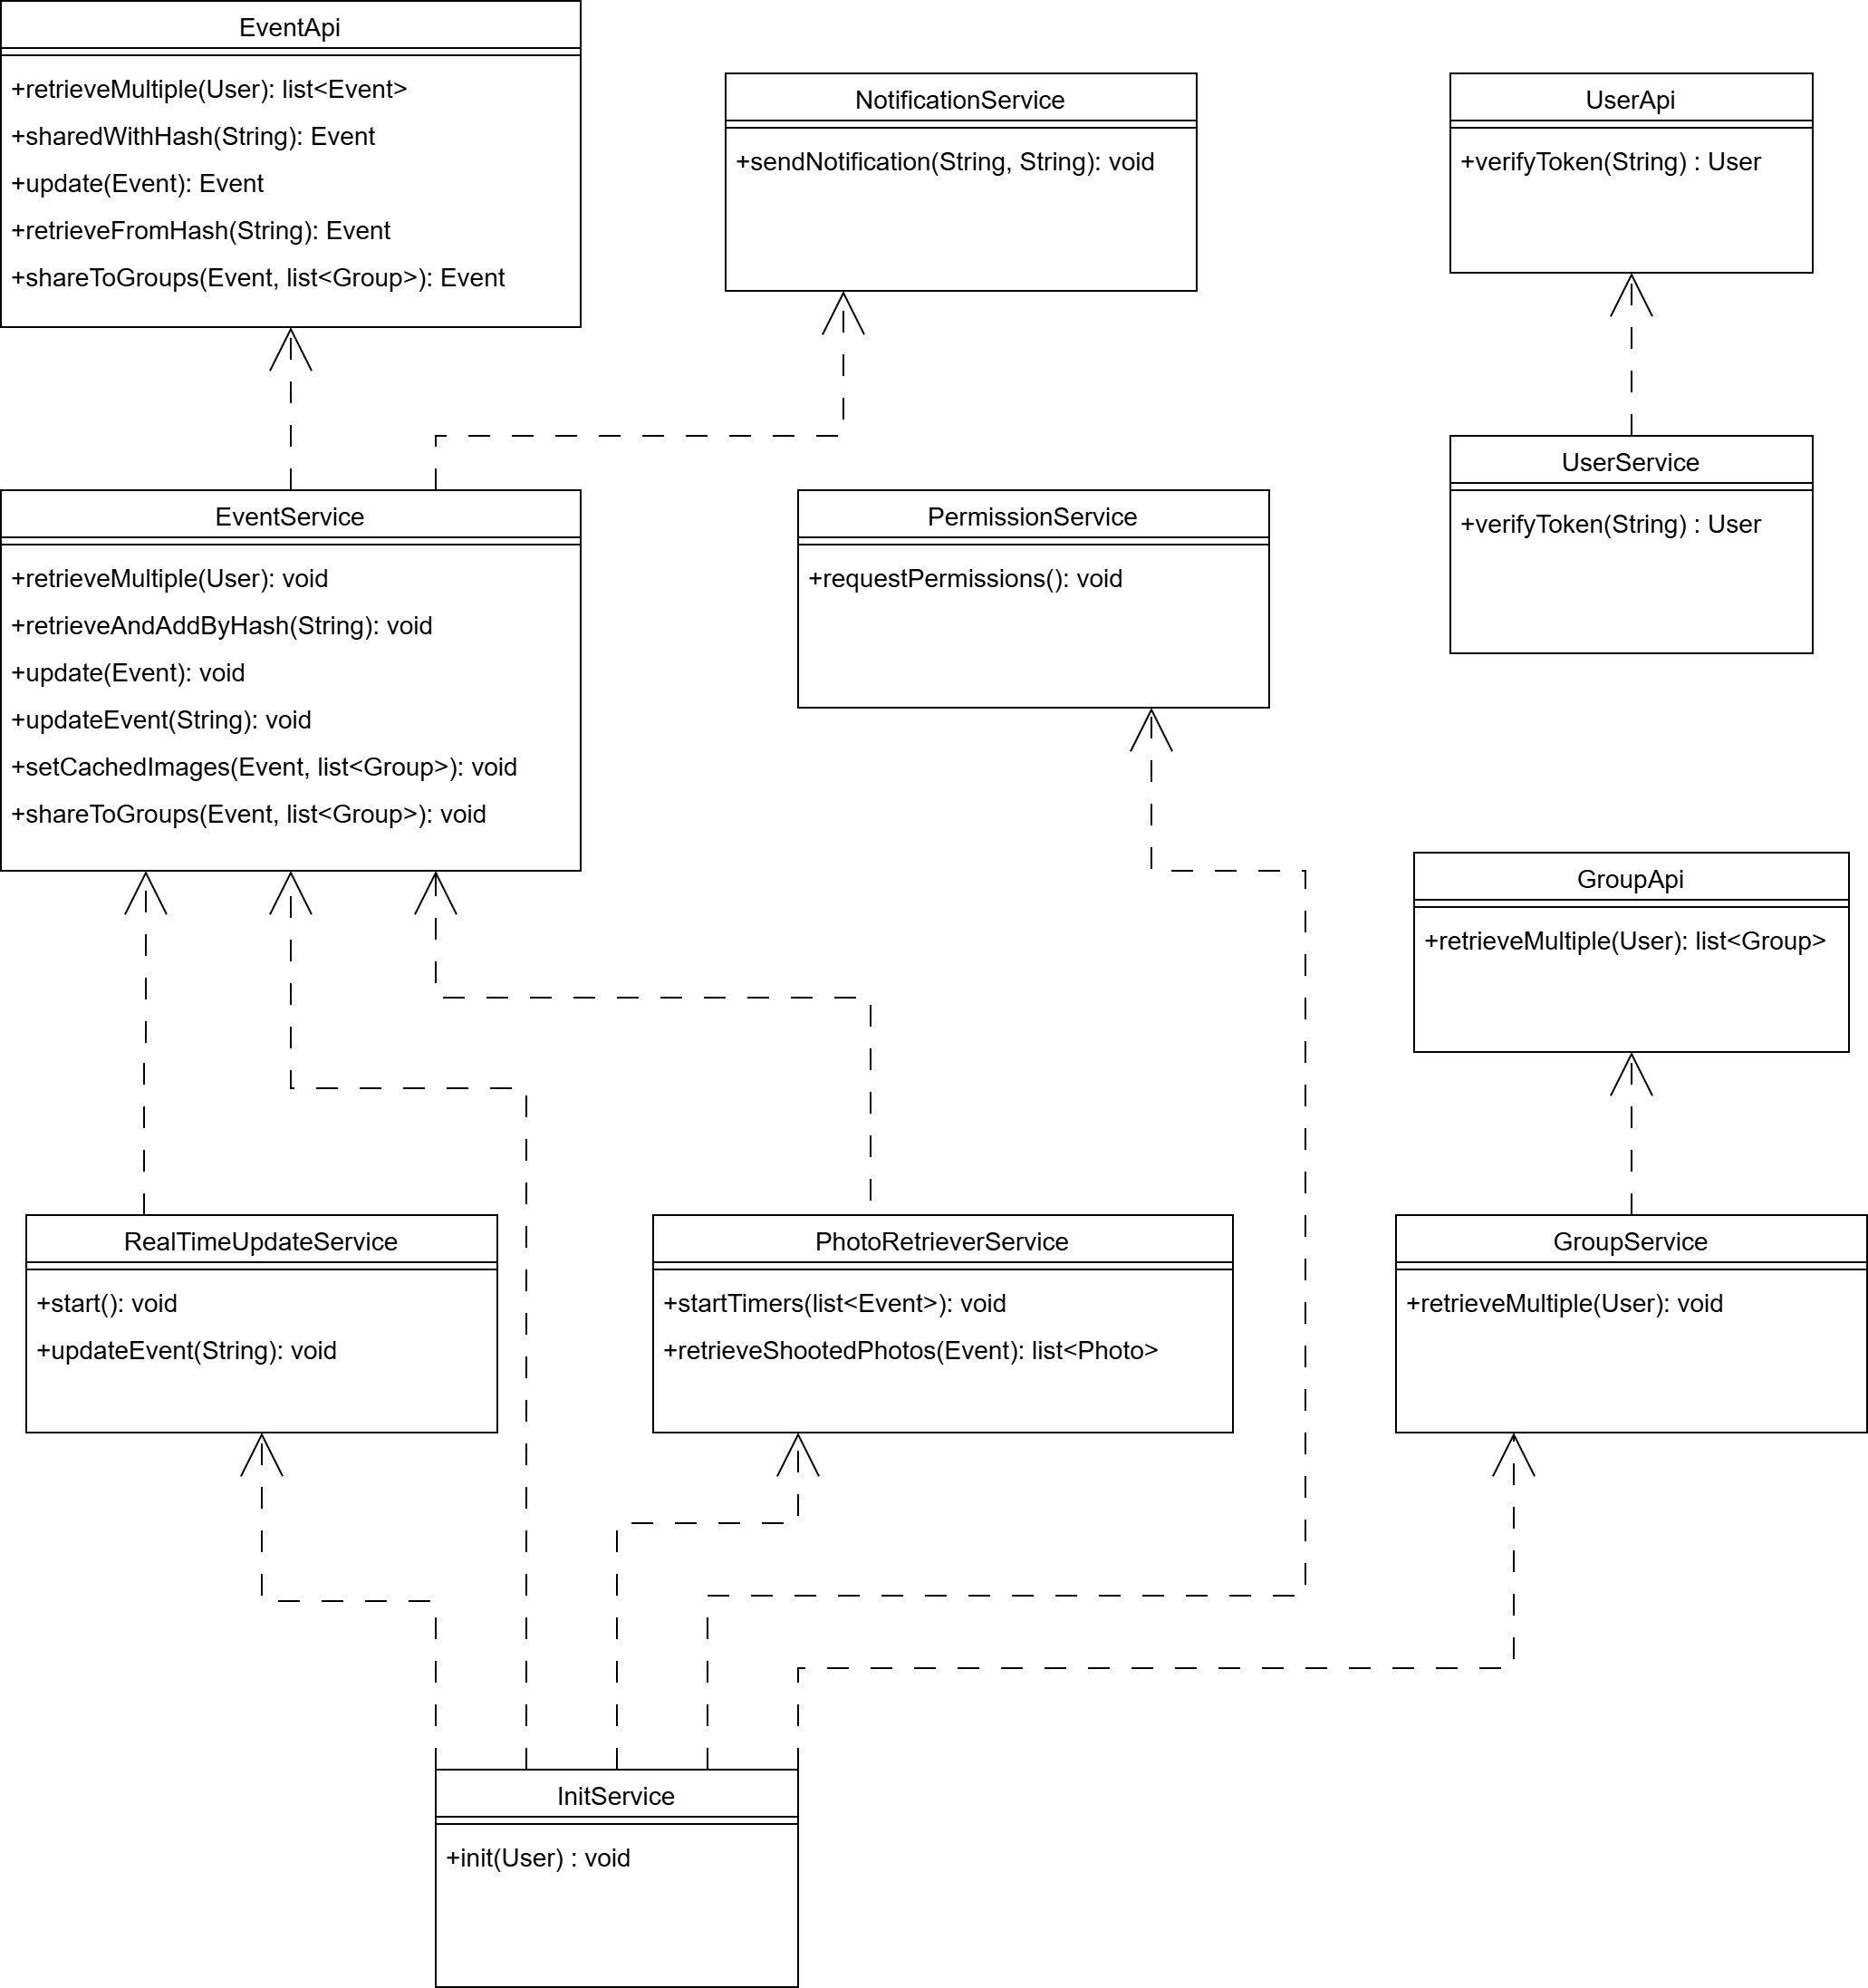
\includegraphics[height=0.72\textheight]{FrontServiceClassDiagram.png}
        \caption{Modello delle classi del client}
    \end{center}
\end{figure}

Non tutte le funzionalità sono correlate direttamente al dominio.
Per questo motivo si creano servizi ausiliari dedicati,
anch'essi separatati in base al ruolo che ricoprono.
\clearpage
Un servizio è stato dedicato all'acquisizione e
al salvataggio dei permessi necessari per operare,
quali l'invio delle notifiche e l'accesso alla galleria.
Mette a disposizione degli altri processi, quindi, 
la conferma dell'accesso ai permessi richiesti o,
in caso non lo si possegga, gestirà il suo ottenimento.\\
\\
L'invio delle notifiche e la ricezione degli aggiornamenti,
per quanto concettualmente simili e strettamente correlati,
sono stati implementati in due componenti differenti.
Le notifiche possono essere infatti richieste anche da altri metodi,
e a ogni aggiornamento potrebbe non corrispondere una notifica.
La ricezione delle modifiche in tempo reale avviene usando il pattern observer,
nel quale il servizio si connette a un canale e rimane in attesa di eventuali messaggi.\\

\begin{figure}[h!]
    \begin{center}
        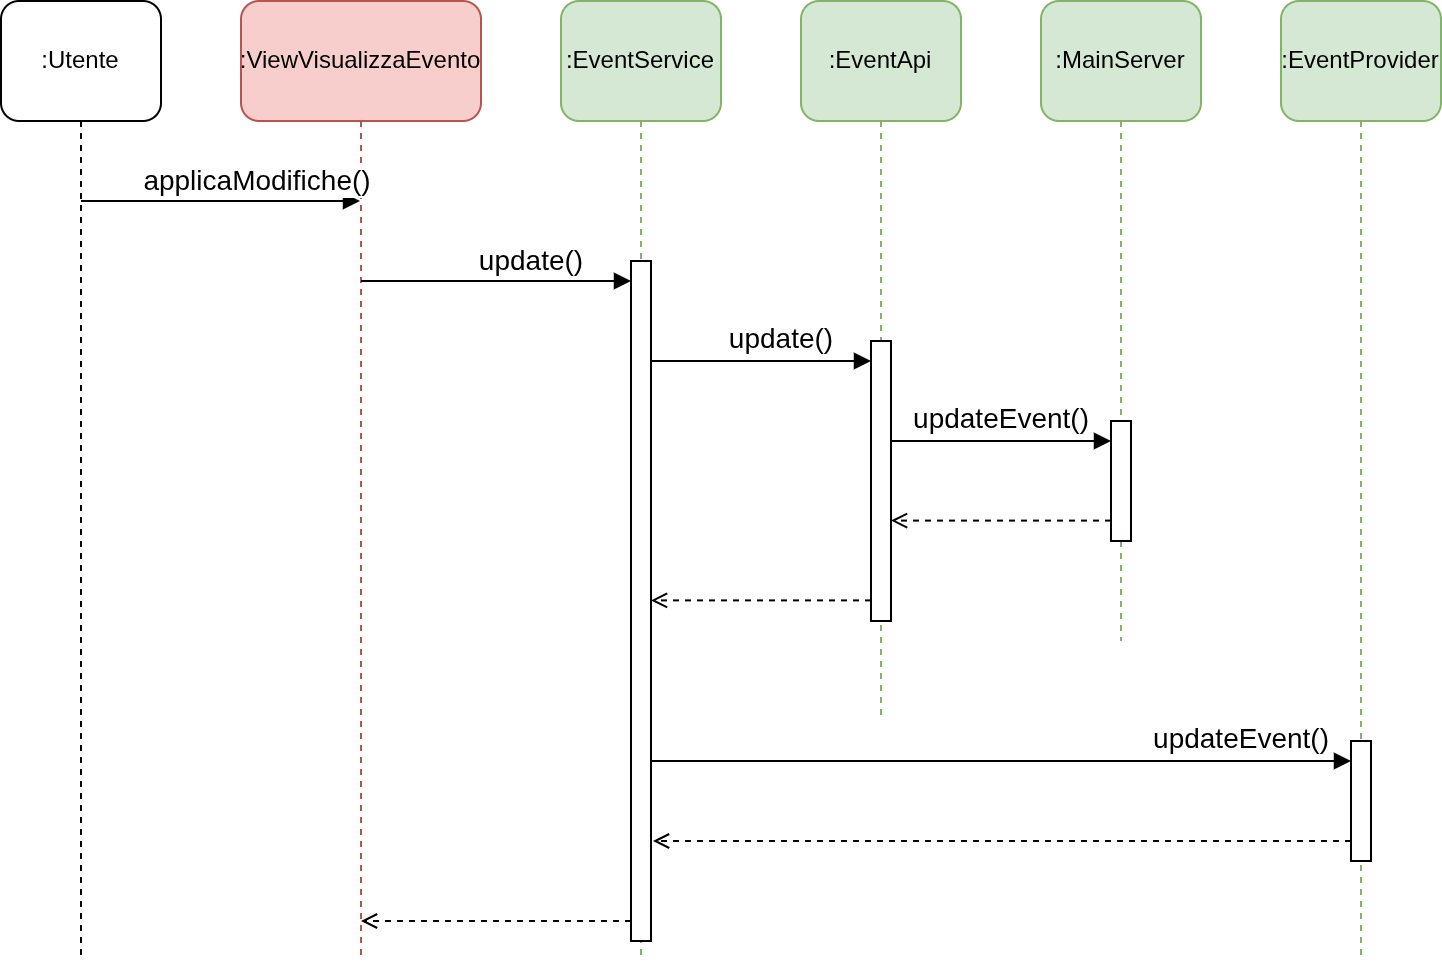
\includegraphics[width=\textwidth]{IIModificaEvento.png}
        \caption{Diagramma di sequenza della modifica di un evento}
    \end{center}
\end{figure}

\clearpage

Il salvataggio in copia dei dati sulla memoria locale
risulta fondamentale per la reattività dell'applicazione,
in quanto permette di ridurre le richieste di dati verso il server
e velocizza il loro recupero.
La memoria locale viene implementata grazie a classi Provider,
create in relazione agli elementi del dominio.
Un'altra funzionalità centrale dell'applicazione è il recupero automatico
delle foto scattate durante l'evento.
Questo richiede la pianificazione di azioni automatiche nel tempo,
così come la scansione della galleria per trovare le immagini interessate.
Sia la gestione locale della memoria che il recupero delle immagini
vedono uno o più componenti dedicati.
La loro realizzazione viene trattata nei capitoli seguenti.\\
\\
Durante l'implementazione della logica applicativa
si sono dovuti affrontare altri problemi quali, degni di nota,
la gestione della condivisione di un evento tramite link e
l'inizializzazione dell'applicazione.\\

\begin{figure}[h!]
    \begin{center}
        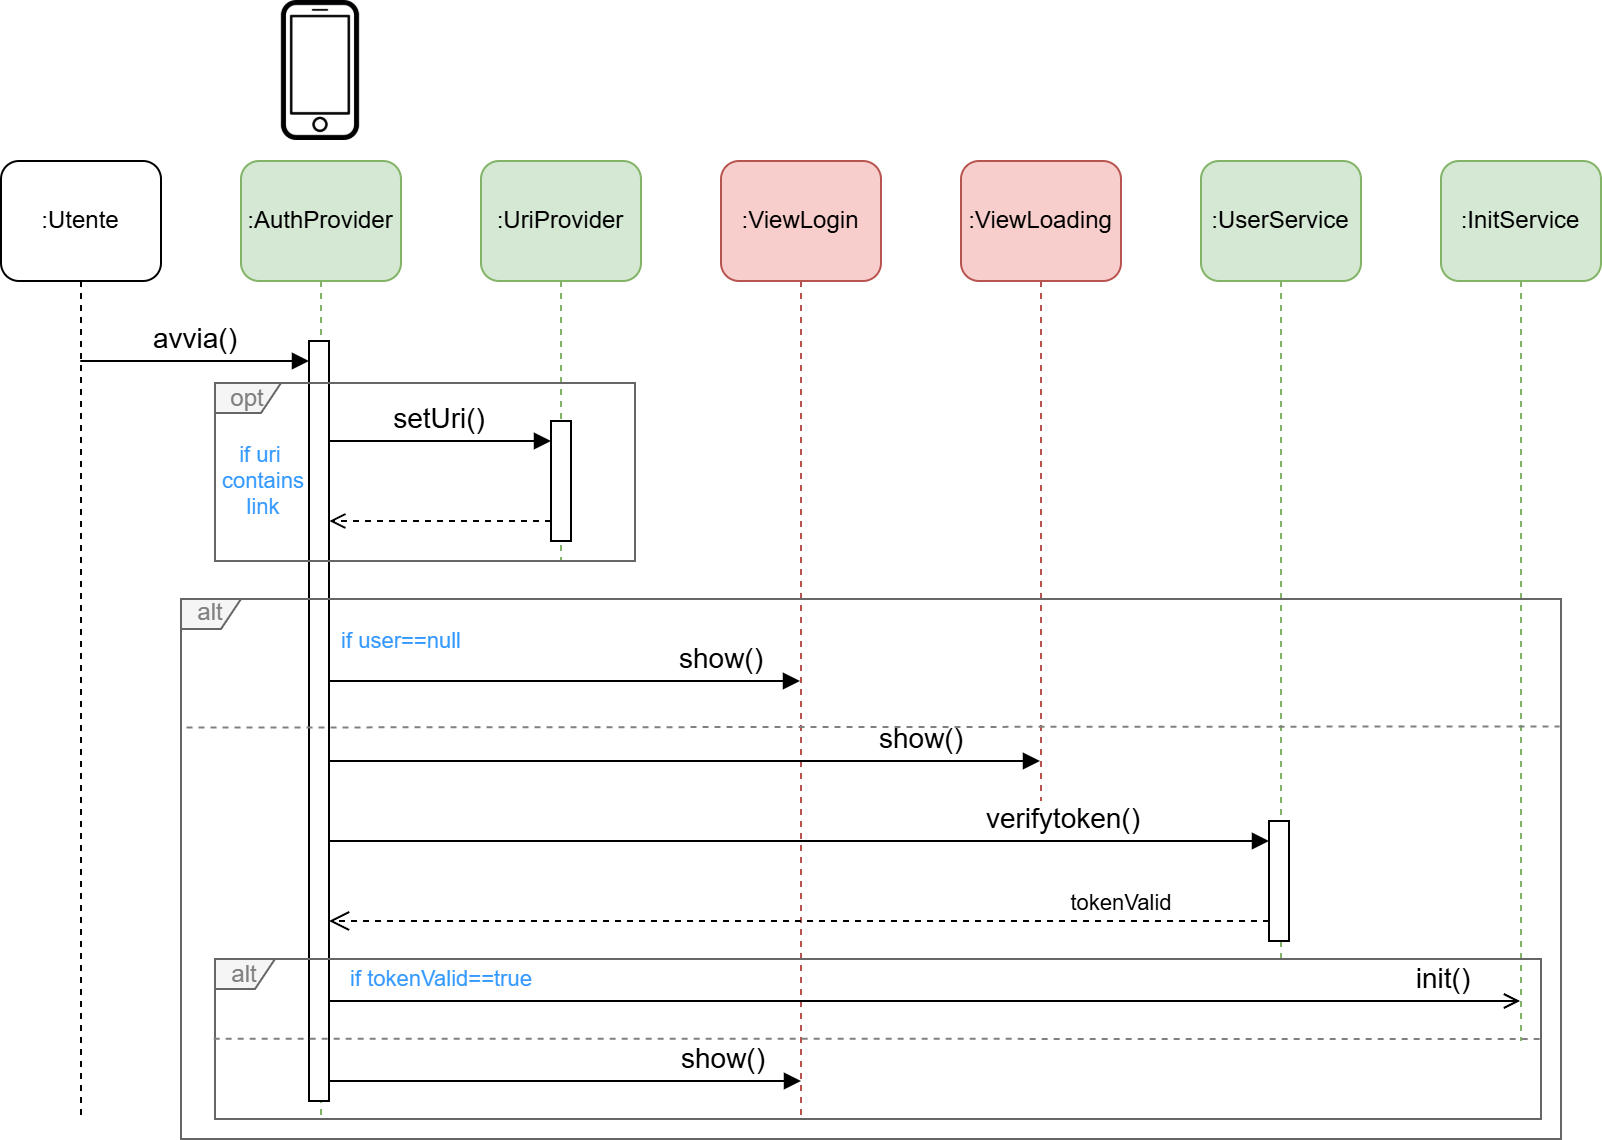
\includegraphics[width=\textwidth]{Avvio.png}
        \caption{Diagramma di sequenza dell'avvio dell'applicazione}
    \end{center}
\end{figure}

La condivisione di un evento tramite link
consiste in due passaggi principali:
la creazione del link stesso e il successivo ritrovamento dell'evento associato.
La generazione del link avviene tramite
l'unione del dominio del server con il codice identificativo dell'evento.\\
\\
All'apertura dell'applicazione tramite link
viene estratto il codice identificativo dell'evento
per la successiva richiesta dei dati al server.
Se l'utente non si è ancora autenticato
il router dell'applicazione lo reindirizza però alla schermata di login,
cambiando il link e perdendo l'informazione allegata.
Per evitare questo problema,
nel momento in cui l'utente accede all'applicazione tramite un link,
le informazioni dell'evento vengono salvate in memoria locale.
Al termine del login, se sono presenti dati salvati,
l'utente verrà indirizzato alla schermata degli eventi proposti,
che recupererà i dati relativi all'evento, per poi mostrarli a video.\\
\\

\begin{figure}[h!]
    \begin{center}
        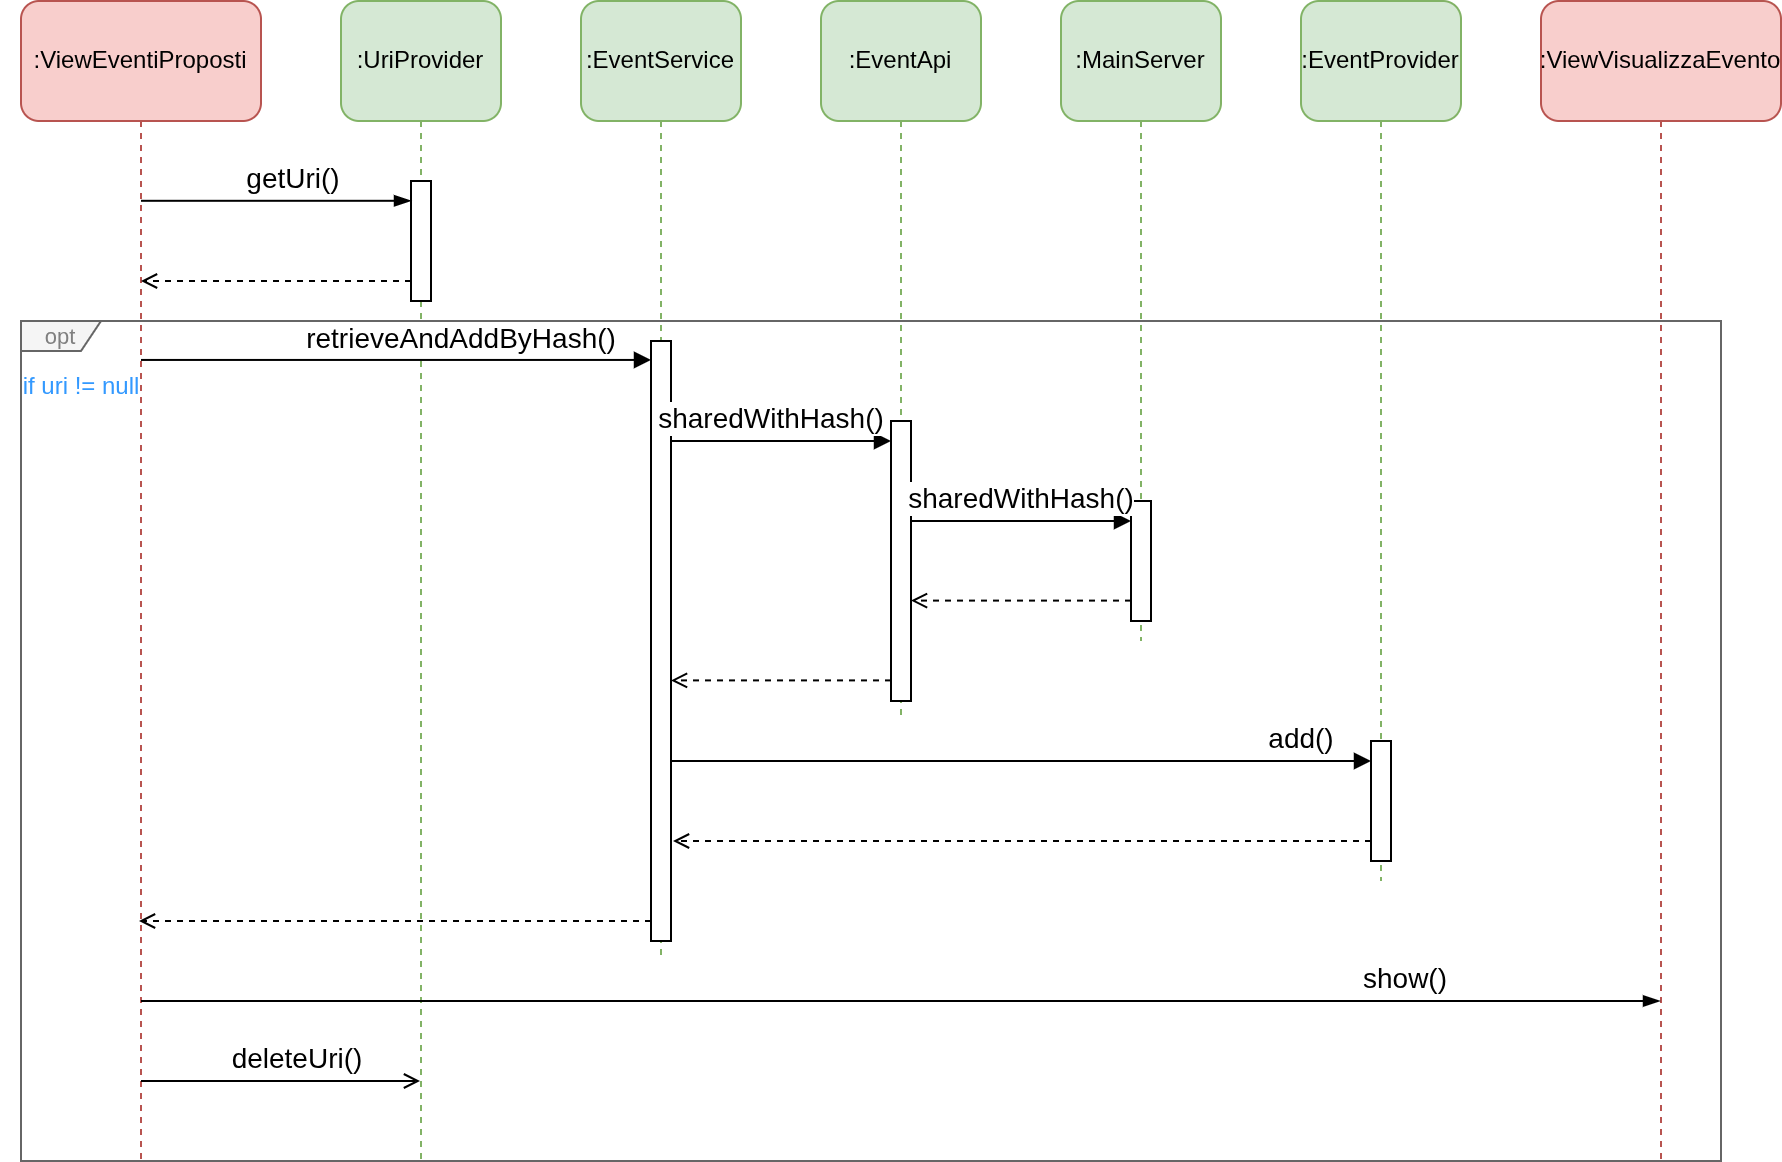
\includegraphics[width=\textwidth]{IIVisualizzaEventiProposti.png}
        \caption{Diagramma di sequenza della visualizzazione dell'evento proposto}
    \end{center}
\end{figure}

\clearpage

La fase di inizializzazione avviene a seguito di un login andato a buon fine.
Parallelamente alla visualizzazione della schermata iniziale
vengono recuperano i dati relativi ai profili associati all'utente
e vengono fatti partire i servizi autonomi.
In particolare, 
vengono controllati i permessi necessari per i quali,
se non ancora concessi, verrà richiesto l'ottenimento.
Viene inoltre avviato il servizio di ricezione degli aggiornamenti,
che si connette al canale relativo all'utente.
Per ogni profilo vengono, sempre in maniera parallela, 
recuperati i gruppi e gli eventi associati.
Al termine della ricezione degli eventi, 
indipendentemente dalle altre richieste,
per ogni evento successivo al momento attuale viene avviato un timer, 
che scatena, al momento giusto, il recupero delle immagini.
Se l'applicazione è stata aperta tramite link di condivisione,
la schermata a cui si verrà reindirizzati sarà quella degli eventi proposti,
altrimenti quella degli eventi confermati.\\
\\

\begin{figure}[h!]
    \begin{center}
        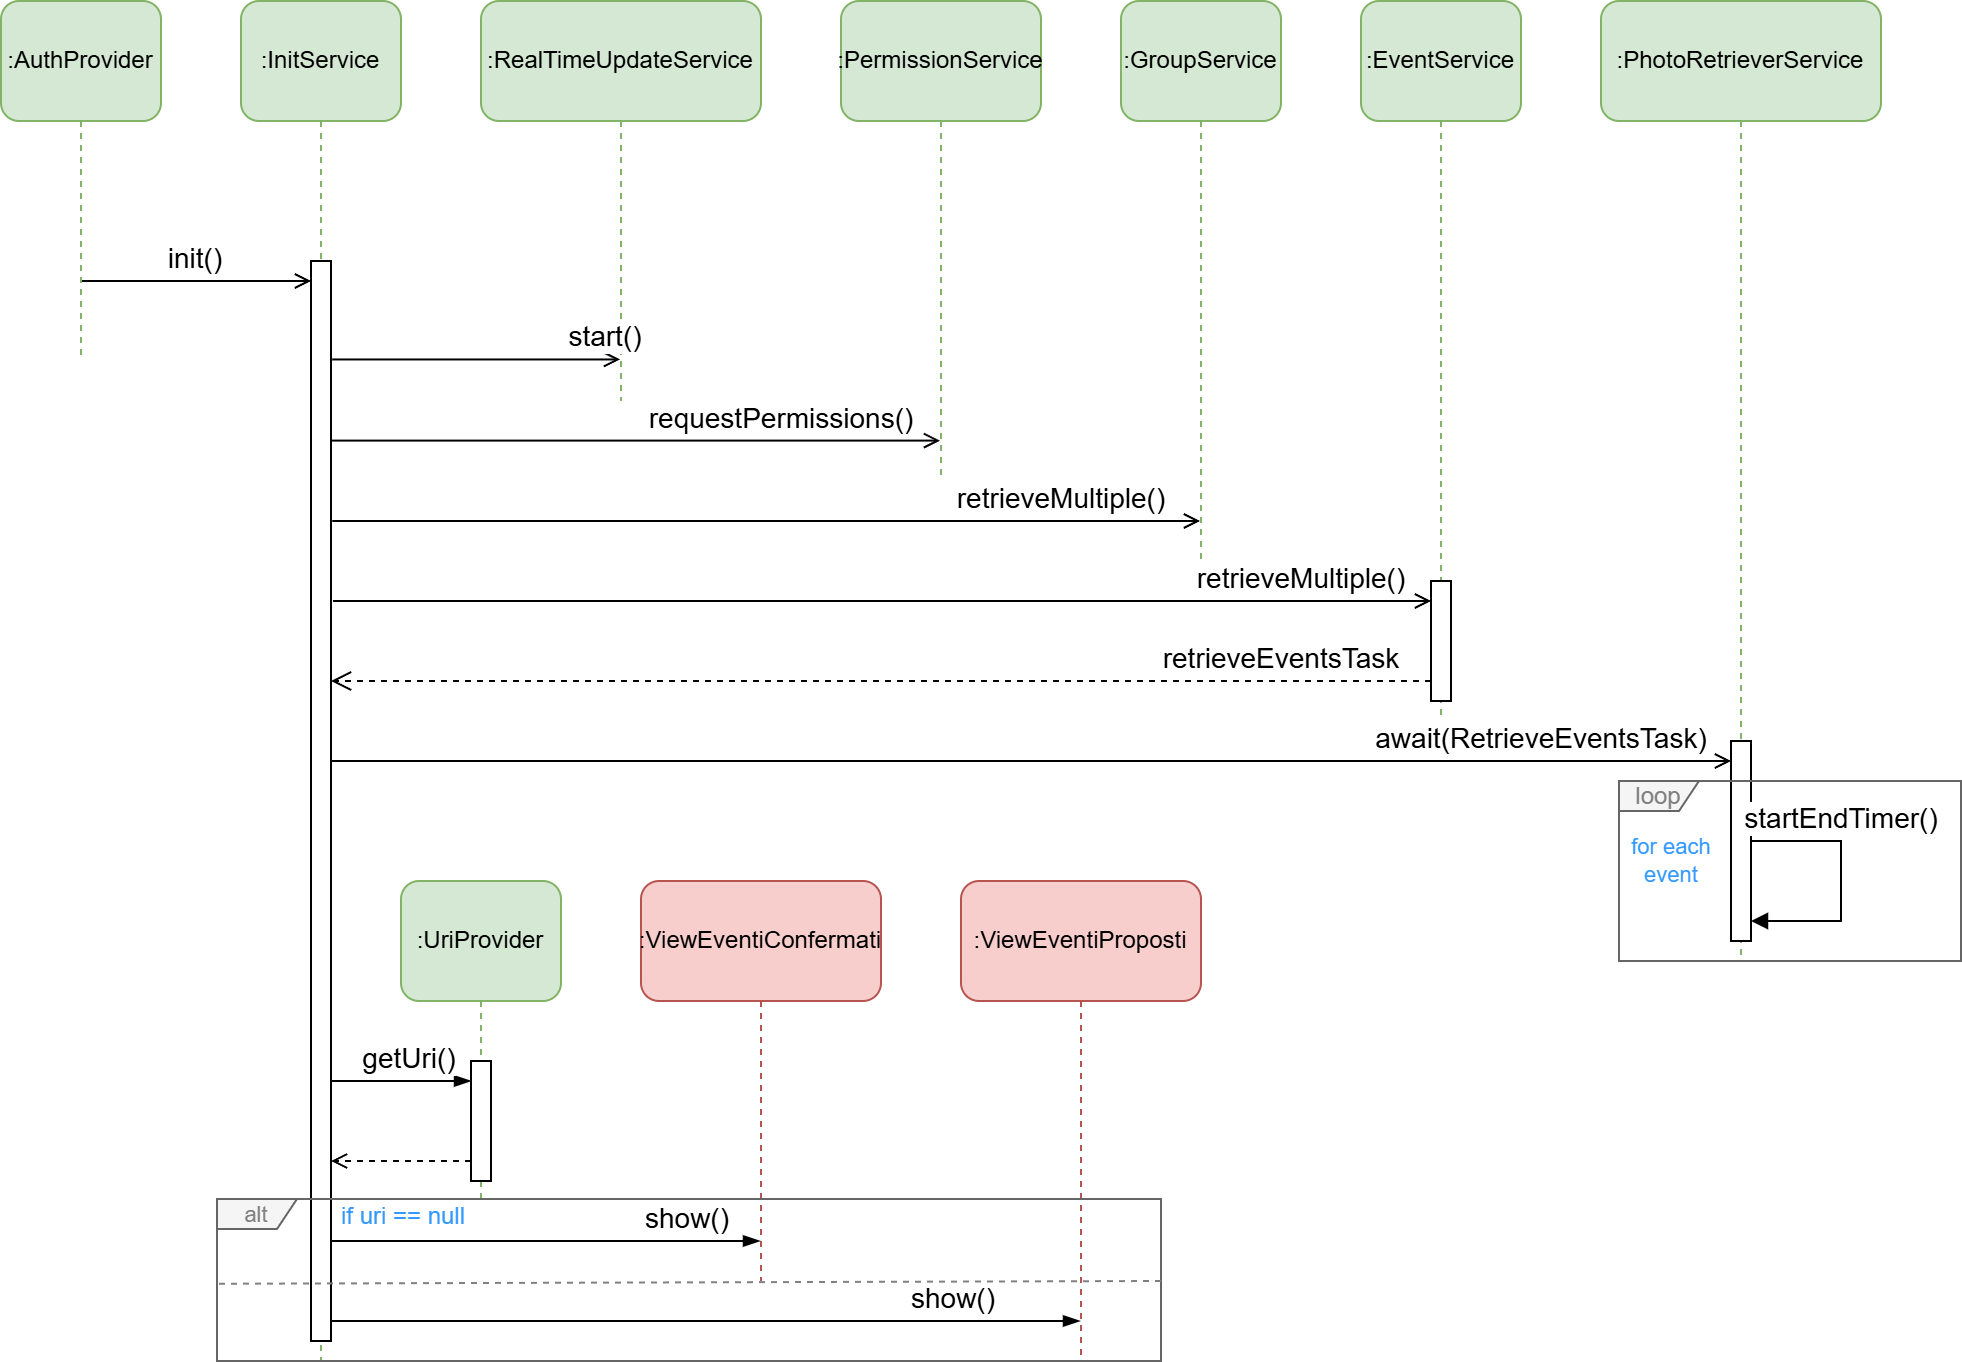
\includegraphics[width=\textwidth]{Init.png}
        \caption{Diagramma di sequenza della fase di inizializzazione }
    \end{center}
\end{figure}


\clearpage

\subsection{Distribuzione del codice verso i dispositivi utente}

Per quanto Flutter consenta di uniformare lo sviluppo e
semplifichi la compilazione del codice per essere eseguito su diverse piattaforme,
alcune configurazioni rimangono comunque dipendenti
dalla tecnologia su cui l'applicazione viene eseguita.
Di conseguenza, 
ogni categoria di dispositivi per la quale si vuole distribuire l'applicazione 
richiede l'introduzione di una manutenzione aggiuntiva.
Oltre alle modifiche derivate dalle dipendenze specifiche,
bisogna anche considerare la distribuzione e la gestione delle versioni.
Per questi motivi, nella fase iniziale dello sviluppo,
nell'ottica di coprire il più ampio mercato possibile con il minor numero di piattaforme,
si è deciso di sviluppare una versione fruibile via web e una per dispositivi Android,
con l'obiettivo di estendere il servizio alle altre tecnologie in un secondo momento.\\
\\
La grafica è stata sviluppata in maniera statica,
ovvero indipendentemente dalle informazioni specifiche dell'utente.
L'interfaccia sviluppata infatti non prevede la creazione dinamica di contenuti:
gli elementi visuali che vengono restituiti rimangono invariati
indipendentemente dall'utente che ne effettua la richiesta.
I dati visualizzati che interessano l'utente corrente
(eventi confermati o proposti, gruppi, profili e via dicendo)
sono recuperati dalla memoria locale del dispositivo o tramite un server terzo.
Questa scelta consente di rendere l'interfaccia grafica completamente
indipendente dall'identità o dal ruolo dell'utente,
consentendo una separazione netta delle responsabilità dei componenti.\\
\\
Da un punto di vista della distribuzione,
le due tecnologie per cui l'interfaccia è stata realizzata
funzionano in modalità completamente diversa.
L'interfaccia web prevede l'utilizzo di un browser utente
che si connette a un server apposito
per ottenere la grafica da visualizzare.
L'interfaccia Android 
(come qualunque interfaccia realizzata per essere eseguita direttamente su un dispositivo)
richiede invece la creazione di un applicativo apposito,
da scaricare e installare sul dispositivo.\\
\\
Per la fruizione del codice web è necessario un server relativamente semplice,
che, grazie alla staticità del sito,
restituisca solo gli elementi necessari per la visualizzazione e l'elaborazione locale,
senza bisogno di modificarli.
La creazione di questo tipo di risorsa usando
\begin{wrapfigure}{o}{0.25\textwidth}
    \centering
    
\includegraphics[height=.12\textheight]{staticwebapp.png}
    Azure Static Web App
\end{wrapfigure}
tecnologie in cloud può avvenire in vari modi,
dall'utilizzo di una macchina virtuale apposita
a soluzioni che utilizzano container.
Tuttavia, Azure mette a disposizione un servizio apposito per queste precise esigenze,
Azure Static Web App (SWA).\newline
Questa risorsa, 
oltre a integrarsi direttamente con il resto dell'ambiente Azure,
garantisce disponibilità e scalabilità in ogni momento,
facendosi carico di gestire la capacità computazionale richiesta.
Permette inoltre, ad esempio, 
il collegamento con servizi di monitoraggio delle performance.
Il consumo delle risorse è infatti calcolato in base alla bandwidth,
ovvero la quantità di dati che viene fornita dal server.
Il piano gratuito prevede i primi cento giga byte di bandwidth inclusi,
che rende il servizio vantaggioso, oltre che pratico.\newline
\par
\begin{wrapfigure}{o}{0.25\textwidth}
    \centering
    
\includegraphics[height=.12\textheight]{blobstorage.png}
    Azure Blob Storage
\end{wrapfigure}
La distribuzione dell'applicativo Android
necessita di un modo per scaricare il file di installazione del programma.
In attesa della pubblicazione dell'applicativo sull'App Store di Android,
che fornirebbe agli utenti la possibilità di trovarlo e installarlo direttamente,
ma che richiede ulteriori passaggi di certificazione e autenticazione,
è stato necessario trovare un'altra soluzione.
Anche in questo caso,
le opzioni per fornire un file tramite cloud ce ne sono tante,
ma la più semplice ed efficace è attraverso l'utilizzo di Azure Blob Storage.\\
\\
Questo servizio consente l'archiviazione e la distribuzione di file di varie tipologie,
fornendo un link diretto per il loro recupero.
Ha un costo che varia in base all'utilizzo,
aggirandosi attorno ai due centesimi per giga byte.
Bilanciando la temporaneità del servizio,
la ridotta quantità di download inizialmente previsti e
la complessità che verrebbe introdotta in caso di utilizzo di un altro servizio,
non è stato ritenuto necessario approfondire ulteriormente la ricerca.\\
\\
Nonostante l'esecuzione del codice presenti alcune dipendenze in base al dispositivo,
la distribuzione non ha introdotto nessuna necessità.
Nessuna modifica del codice è stata quindi dovuta alla scelta della tecnologia usata per
la loro distribuzione.\\
\\
Per garantire un processo di aggiornamento efficiente e automatizzato,
sia il codice distribuito sulla web app che l'applicativo ospitato nel container
vengono gestiti tramite GitHub Actions.
Le Github Actions sono funzionalità offerte da Github,
che è il sito dove viene salvato il codice.
In particolare, 
a ogni nuova versione del codice 
sia la Static Web App che il Blob Storage vengono notificati,
modificando il loro contenuto.
Questo consente di offrire un servizio aggiornato
riducendo al minimo i tempi richiesti per applicare le modifiche.
ASWA gestisce in autonomia il collegamento con la repository Github,
mentre per aggiornare l'applicazione su Android è stato necessario crearne una appositamente.\\
\\
In caso di aggiornamento,
la fruizione dell'interfaccia tramite browser non necessita di nessuna manutenzione
in quanto si aggiorna automaticamente a ogni accesso.
Per l'applicativo su dispositivo mobile è invece necessaria una nuova installazione manuale.
Per questa ragione, gli utenti dell'applicazione verranno notificati tempestivamente
ogni volta che sarà disponibile una nuova versione.\\
\\

\begin{figure}[htbp]
    \begin{center}
        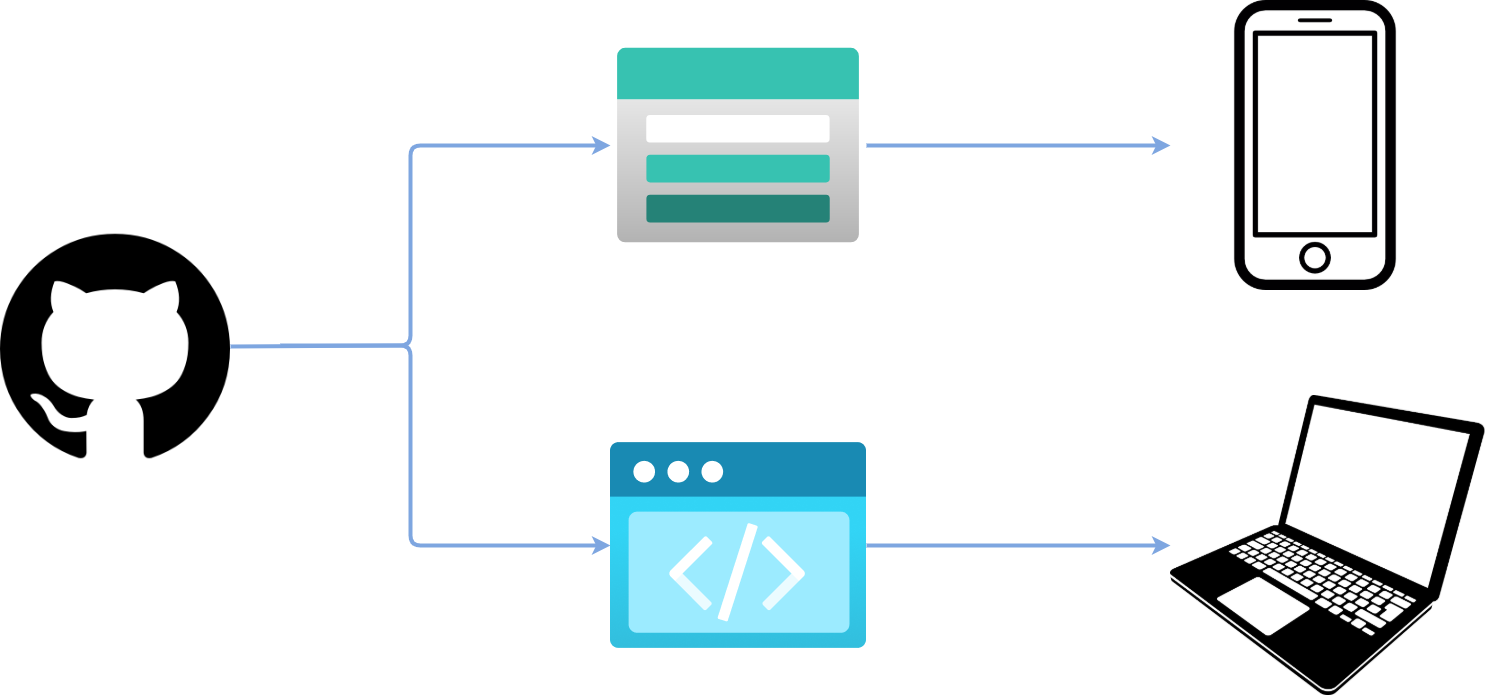
\includegraphics[height=0.28\textheight]{DeployFront.png}
        \caption{Diagramma di aggiornamento e distribuzione del client}
    \end{center}
\end{figure}
\clearpage

%\section{Creazione del server principale}

Il server principale è il componente con il compito 
di ricevere tutte le richieste dai client,
elaborarle e restituire le informazioni volute,
eventualmente a seguito di un'interrogazione verso la persistenza centrale.
Per poter essere in grado di rispondere a un numero sempre maggiore di utenti,
idealmente senza che questo impatti sul tempo di risposta o sulle performance in generale,
deve essere implementato in maniera tale da poter permettere un'esecuzione distribuita,
riducendo al minimo le dipendenze che possano minarne la duplicazione.\\
\\
Per soddisfare questo tipo di esigenza
esistono servizi definiti come Function as a Service (FaaS).
I FaaS sono servizi serverless,
ovvero la loro gestione hardware è completamente delegata al gestore del cloud;
il cui scopo è quello di duplicare ed eseguire il progetto,
suddiviso e implementato attraverso molteplici funzioni.
Ogni funzione consiste in un'unità indipendente di codice,
e in quanto tale crea la possibilità di essere eseguita 
in un ambiente di esecuzione unico per ogni richiesta.
Questa caratteristica, 
combinata con la virtualizzazione dell'ambiente di esecuzione,
consente una scalabilità potenzialmente illimitata.\\
\\
L'indipendenza della funzione dipende dalla relazione 
con le altre parti del progetto e dalla sua natura stateless.
L'esecuzione di una funzione infatti,
oltre a dover essere limitata rispetto a qualunque dipendenza logica che possa dover essere condivisa,
deve essere svincolata dalle informazioni sullo stato o sulla sessione.
Queste caratteristiche, per loro natura, 
non possono essere garantite dal servizio,
e sono quindi una responsabilità di chi deve svilupparle.\\
\\
Per assicurarne l'autonomia,
le funzioni dovranno essere implementate seguendo il principio di singola responsabilità.
Ogni Function adempirà un solo compito specifico,
creando una restrizione delle dipendenze e
garantendo il minimo utilizzo di risorse necessarie per rispondere alla richiesta.
Inoltre, viene così semplificata la creazione e la manutenzione del codice,
riducendo il controllo dell'esecuzione all'esito del tentativo di risoluzione del singolo problema.
\clearpage
\subsection{Individuazione del servizio adatto}

I gestori in cloud che offrono servizi FaaS sono limitati.
Escludendo i fornitori improntati allo sviluppo di applicazioni principalmente front-end,
i fornitori sul mercato con servizi testati e maturi sono
Amazon Web Services con AWS Lambda, 
Azure con Azure Functions e
Google Cloud Provider con Google Cloud Functions.
Tuttavia, queste tre soluzioni si assomigliano particolarmente.
Nonostante siano state tutte implementate usando una tecnologia proprietaria,
le proprietà computazionali, il supporto ai linguaggi e il costo risultano molto simili.\\
\\
Presentano tutti una granularità relativa
alla scalabilità delle richieste a livello di funzione,
ovvero permettono di duplicare il solo codice necessario per l'esecuzione della funzione richiesta.
Il supporto ai linguaggi è molto esteso,
ma offrono tutti comunque la possibilità di creare un runtime personalizzato,
di fatto supportando tutte le tecnologie.\\

\begin{longtable} {|P{3.5cm}|P{3.7cm}|P{3.7cm}|P{3.7cm}|}
    \hline
                                                    & \textbf{AWS Lambda}                                         & \textbf{Azure Functions} & \textbf{Google Cloud Functions} \\
    \hline
    \endhead
    Linguaggi supportati                            &
    Node.js, Python, Java, C\#, Go, PowerShell, Ruby, PHP
                                                    &
    Node.js, Python, Java, C\#, PowerShell, F\#, PHP
                                                    &
    Node.js, Python, Java, C\#, Go, F\#, Visual Basic                                                                                                                          \\
    \hline
    Runtime Personalizzato                          & Sì, tramite i custom deplyment packages o AWS Lambda Layers &
    Sì, grazie ai custom handlers                   &
    Sì, tramite immagini Docker personalizzate                                                                                                                                 \\
    \hline
    Massimo tempo di esecuzione                     &
    15 minuti                                       &
    Dai 10 ai 60 minuti, in base al piano di pagamento
                                                    &
    60 minuti per le richieste HTTP, 9 minuti per le richieste a eventi                                                                                                        \\
    \hline
    Massima memoria dedicata a funzione             &
    10 GB                                           &
    Da 1.5 GB a 14 GB in base al piano di pagamento &
    4 GB                                                                                                                                                                       \\
    \hline
    Tempo medio di attesa prima di essere spento    &
    Dai 5 ai 7 minuti                               &
    Tra i 20 e i 30 minuti                          &
    15 minuti                                                                                                                                                                  \\
    \hline
    Tempo medio di cold-startup                     &
    Generalmente sotto il secondo                   &
    Non oltre i 5 secondi                           &
    Da mezzo secondo a 2 secondi                                                                                                                                               \\
    \hline
    Orchestrazione                                  &
    Sì, tramite AWS Step Functions                  &
    Sì, tramite Durable Azure Functions             &
    Sì, tramite GCP workflow                                                                                                                                                   \\
    \hline
    \textbf{Costi}                                  &                                                             &                          &                                 \\
    \hline
    Richieste gratuite mensili                      &
    400.000 GB-seconds                              &
    400.000 GB-seconds                              &
    400.000 GB-seconds                                                                                                                                                         \\
    \hline
    Tempo di esecuzione gratuita al mese            &
    1 milione                                       &
    1 milione                                       &
    2 milioni                                                                                                                                                                  \\
    \hline
    Costo della richiesta al consumo                &
    \$0.20 per milione                              &
    \$0.20 per milione                              &
    \$0.40 per milione                                                                                                                                                         \\
    \hline
    Costo di esecuzione al consumo                  &
    \$0.000016 per GB-seconds                       &
    \$0.000016 per GB-seconds                       &
    \$0.0000125 per GB-seconds                                                                                                                                                 \\
    \hline
    Arrotondamento della durata                     &
    1 millisecondo                                  &
    1 millisecondo                                  &
    100 millisecondi                                                                                                                                                           \\
    \hline
    \caption{Caratteristiche delle principali FaaS}
\end{longtable}

La principale differenza tra queste soluzioni
risulta nel tempo necessario in caso di start up,
ma bisogna notare che,
oltre a essere solo una fase particolare del suo ciclo di vita,
dipende molto dal linguaggio di programmazione,
dalle dipendenze e dalla dimensione del progetto.
Viene inoltre mitigato dal tempo di attesa 
per il quale le istanze rimangono accese pronte a ricevere richieste e
dalla quantità degli utenti attivi che,
generando un flusso continuo di richieste,
contribuiscono a diminuire la frequenza dello spegnimento.\\
\\
Essendo le differenze tra un servizio e l'altro minime,
sia a livello di costi che di prestazioni,
ed essendo il progetto improntato su Azure,
la scelta della tecnologia su cui implementare il server principale
è ricaduta sulle Azure Functions.\\

\subsection{Scelte progettuali derivate dall'utilizzo delle Azure Functions}

L'utilizzo di un servizio FaaS
comporta un approccio particolare per la scrittura del codice.
A differenza di un programma normale,
dove l'esecuzione del programma è indipendente dalla ricezione di un evento,
nelle FaaS l'invocazione di un processo avviene esplicitamente a partire da un fattore esterno
(che sia una richiesta HTTP o il messaggio in una coda).
Non bisogna più preoccuparsi di come far interagire le parti dell'applicazione,
ma piuttosto di come rispondere nella maniera più efficiente possibile a tanti singoli problemi.
Ogni funzione dovrà essere implementata come entità autonoma rispetto al resto del sistema,
con l'unica responsabilità di rispondere a un solo incarico specifico.\\
\begin{wrapfigure}{o}{0.25\textwidth}
    \centering
    
\includegraphics[height=.12\textheight]{functions.png}
    Azure Functions
\end{wrapfigure}
La difficoltà principale del procedimento sussiste nell'individuare i singoli compiti
in cui suddividere l'applicazione.
Raramente una richiesta può essere soddisfatta in un unico passaggio,
e non è quindi automatico che a una Function corrisponda una sola parte di codice,
soprattutto in quanto alcune richieste potrebbero avere alcune parti in comune
(ad esempio, l'autenticazione è necessaria alla maggior parte delle richieste).
Nel caso in cui una richiesta si componga di più passaggi logici,
per poterli racchiudere in un'unica Function bisogna analizzarne la relazione.\\
\par
Innanzi tutto ogni passaggio deve essere implementato
sempre in maniera indipendente e stateless come richiesto alle Azure Function.
A questo punto è necessario però che tutti i passaggi siano in diretta successione,
e che il fallimento di uno solo di questi comporti il fallimento di tutta la funzione.
In caso contrario, è sconsigliato raggrupparle in un'unica funzione,
quanto piuttosto suddividerli in altre piccole funzioni
(con le stesse proprietà di cui sopra),
per poi coordinarle tramite l'utilizzo di un orchestratore o di code di eventi.\\
\\
L'orchestratore è una funzione che ha la caratteristica
di poterne invocare e controllare altre.
Consente di gestire efficacemente scenari
in cui è richiesta un'esecuzione particolare delle operazioni, sia essa sequenziale o parallela,
dove è necessario effettuare tentativi aggiuntivi in caso di errore o fallimento o
si richiede l'attesa del completamento di operazioni con un tempo di esecuzione prolungato.
Tuttavia, la natura stateless e l'accoppiamento debole tra orchestratore
e le Function in esecuzione causano un tempo di risposta delle richieste più elevato.\\
\\
Integrato all'interno delle Azure Functions,
Azure Durable Function consente la creazione di un orchestratore,
incaricato di gestire l'ordine, lo stato,
il ciclo di vita e le risposte delle varie Function coinvolte nell'elaborazione della richiesta,
mantenendo un'architettura indipendente e scalabile.\\
\\
Il coordinamento tramite code di eventi prevede 
invece l'invio di un evento al sistema
durante l'esecuzione della prima funzione,
nel momento in cui questa abbia terminato la sua responsabilità diretta
e possa delegare ulteriori procedimenti.
L'evento verrà aggiunto in coda,
per poi invocare una seconda funzione nel momento in cui sarà preso in carico.
Si consente così di separare logicamente le funzioni tra loro
senza introdurre ulteriori logiche e garantendo un tempo di risposta alla prima funzione minimo.
Questo approccio introduce però alcune problematiche.\\
\\
Disaccoppiando le due funzioni la prima
non ha conoscenza sull'esito della seconda,
ed è quindi necessario che la funzione invocata dalla coda
non svolga un compito essenziale
o che siano previste logiche di controllo,
rilancio o segnalazione dell'esito.
La possibilità che la stessa funzione
venga eseguita più volte con lo stesso messaggio
richiede che il suo comportamento sia idempotente,
ovvero che la sua eventuale esecuzione duplicata non impatti sul risultato finale.
Inoltre l'invocazione verrà così considerata come doppia,
andando a influire sui costi totali.\\
\\
Come linguaggio di programmazione per lo sviluppo delle Function è stato utilizzato C\#.
La consapevolezza che sia l'ambiente di sviluppo di C\#,
ovvero il framework .Net, sia la piattaforma Azure
siano entrambi sviluppati e mantenuti dalla stessa azienda, Microsoft,
garantisce elevati livelli di stabilità,
supporto e coordinamento delle tecnologie adottate.\\
\\
Azure Functions in ambiente .Net supporta due modelli di esecuzione e sviluppo:
in-process worker o isolated worker.
Il worker è il processo all'interno dell'applicativo che gestisce 
l'esecuzione delle funzioni in risposta alle richieste.
Nella modalità in-process,
il worker viene eseguito all'interno dello stesso processo 
dell'host che lo genera,
riducendo la quantità di allocazione delle risorse necessarie
ma condividendo l'ambiente di esecuzione.
Nel modello isolated invece
il worker esegue le funzioni in un secondo un processo,
garantendo maggiore isolamento e aumentando il controllo sulle funzioni.\\
\\
Inoltre, il modello isolated worker offre ulteriori vantaggi
grazie al maggiore supporto fornito.
Innanzi tutto esso prevede una maggiore compatibilità nel tempo,
grazie al più ampio numero di versioni del framework .Net a disposizione.
Il modello in-process, differentemente, 
è limitato alle sole versioni con supporto a lungo termine.
In secondo luogo il supporto per la creazione di middleware personalizzati
permette l'elaborazione di un codice intermedio 
tra la chiamata e l'esecuzione della funzione,
funzionalità invece non disponibile nel modello in-process.
Considerati questi vantaggi, 
le funzioni sono state sviluppate utilizzando il modello isolated worker
per garantire maggiore flessibilità, 
compatibilità e modularità dell'architettura.\\
\\
Lo sviluppo è stato condotto utilizzando Visual Studio Code,
programma open source sviluppato dalla stessa Microsoft per la creazione di codice.
Visual Studio Code permette l'integrazione con molteplici estensioni 
fornendo il supporto per la maggior parte delle tecnologie.
In particolare, grazie alle estensioni dedicate al provider Azure,
è possibile collegare il proprio ambiente di lavoro direttamente con i servizi in cloud.
Il legame così creato consente un aggiornamento immediato e intuitivo del codice,
gestito interamente dal programma.
\clearpage


\subsection{Implementazione della logica applicativa}
Per quanto ogni funzione ricopra un unico compito,
alcune parti della sua risoluzione possono essere condivise con altre.
Per questo motivo,
la logica applicativa è stata suddivisa 
in metodi che risolvono una specifica esigenza logica,
che saranno poi chiamati dalle funzioni quando necessario.
I metodi vengono quindi raggruppati in classi in base all'inerenza dei loro scopi,
concentrando il codice che condivide le stesse necessità e uniformando il suo stile.
Le dipendenze vengono così inizializzate un'unica volta a livello di classe,
creando un software più ordinato.\\
\begin{figure}[h!]
    \begin{center}
        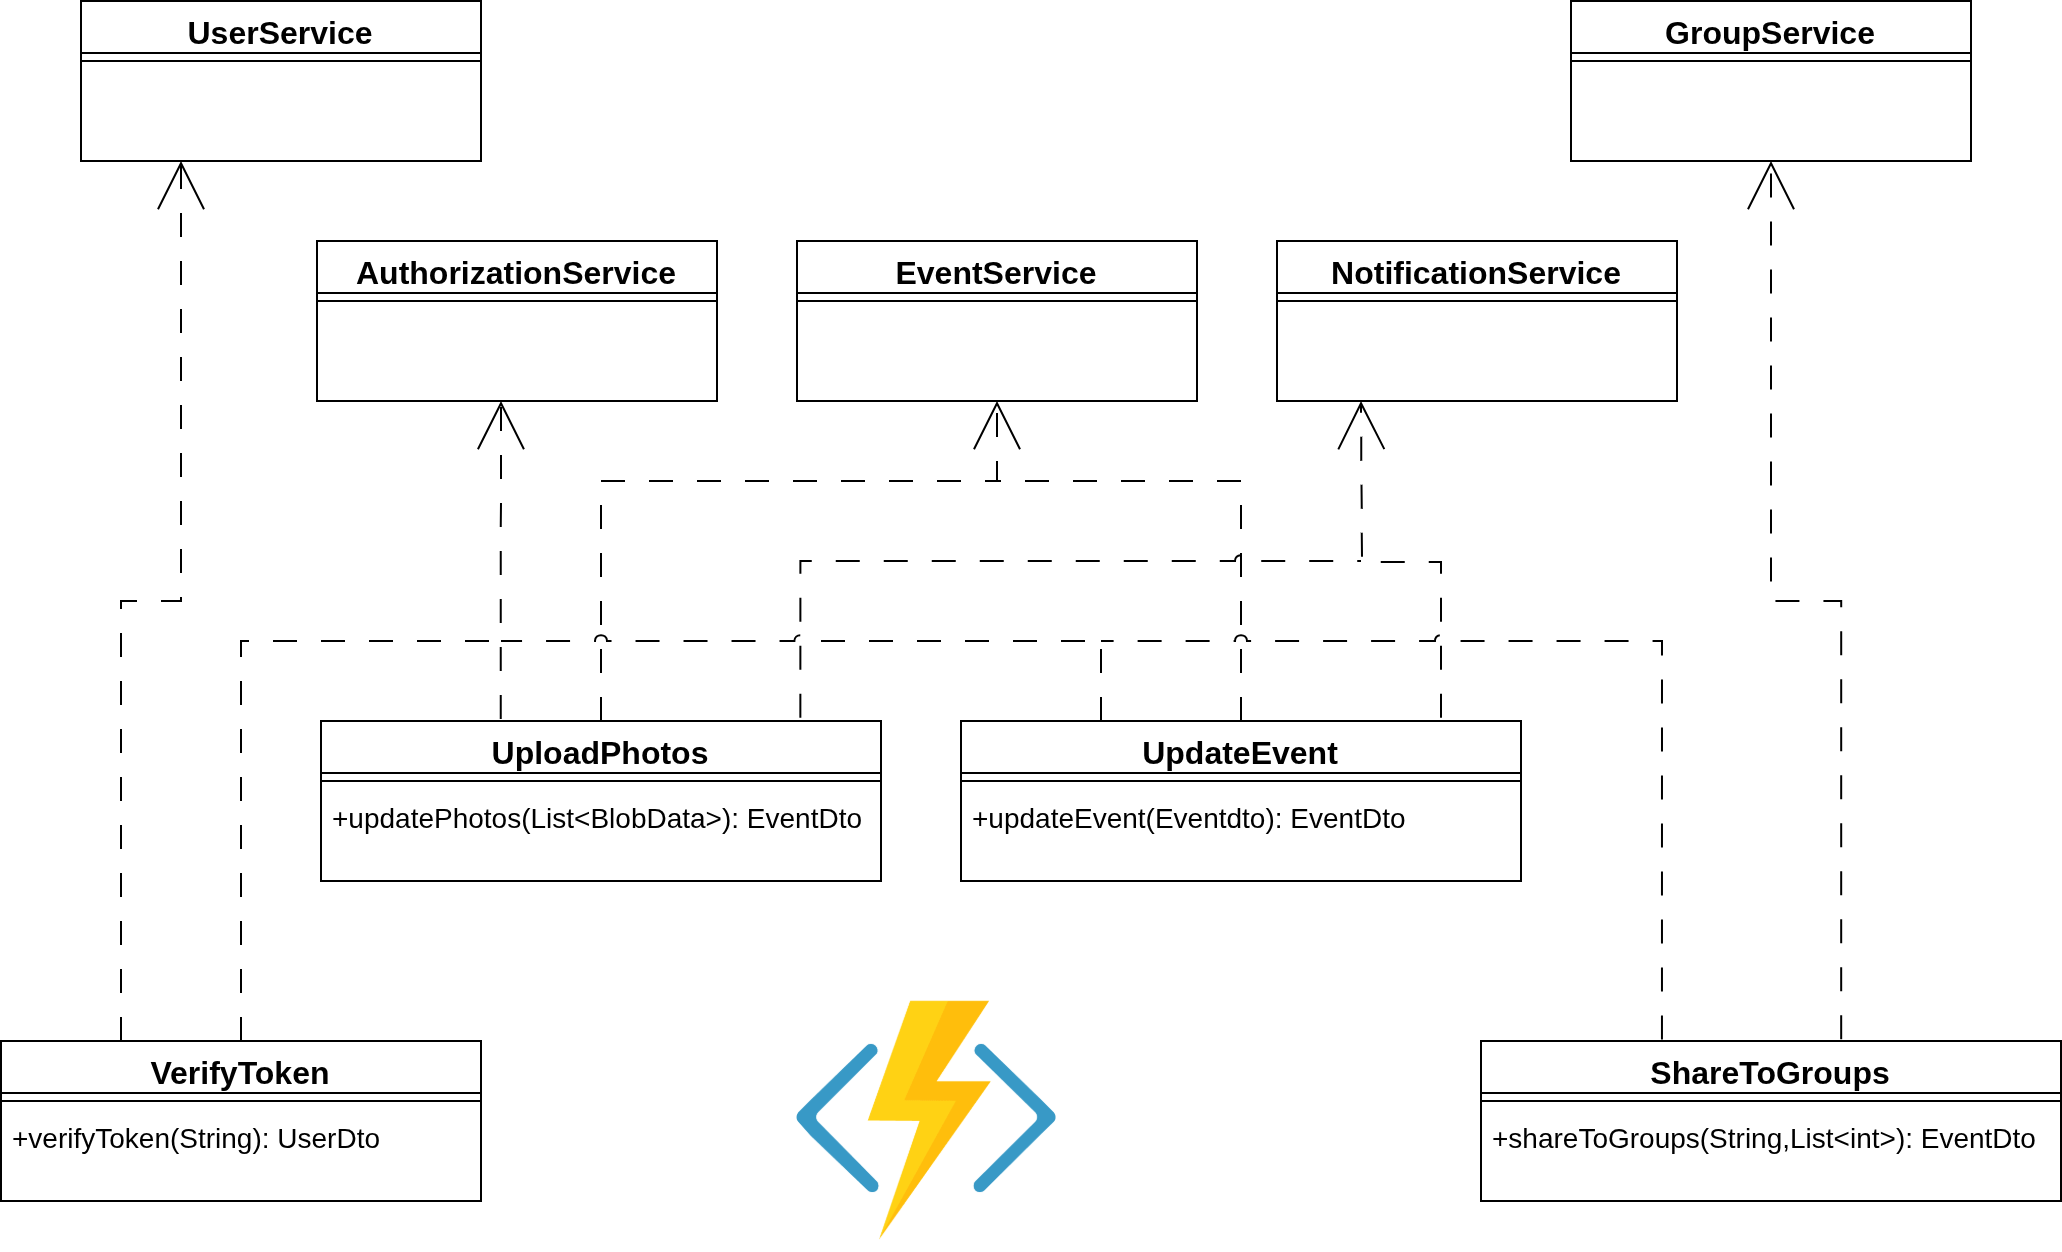
\includegraphics[width=\textwidth]{FunctionClassDiagram.png}
        \caption{Modello delle relazioni tra Functions e i servizi usati}
    \end{center}
\end{figure}

Usando la stessa modalità di suddivisione delle responsabilità
seguita per implementare l'applicativo utente,
le classi sono state sviluppate tenendo conto delle divisioni del dominio
e di ulteriori responsabilità specifiche.
Per ogni elemento principale del dominio è stata sviluppata
una classe service che implementa le operazioni relative,
mentre, per compiti che richiedono particolare attenzione o 
che astraggono l'interazione con una particolare risorsa,
vengono implementate classi apposite.\\
\clearpage
\begin{figure}[h!]
    \begin{center}
        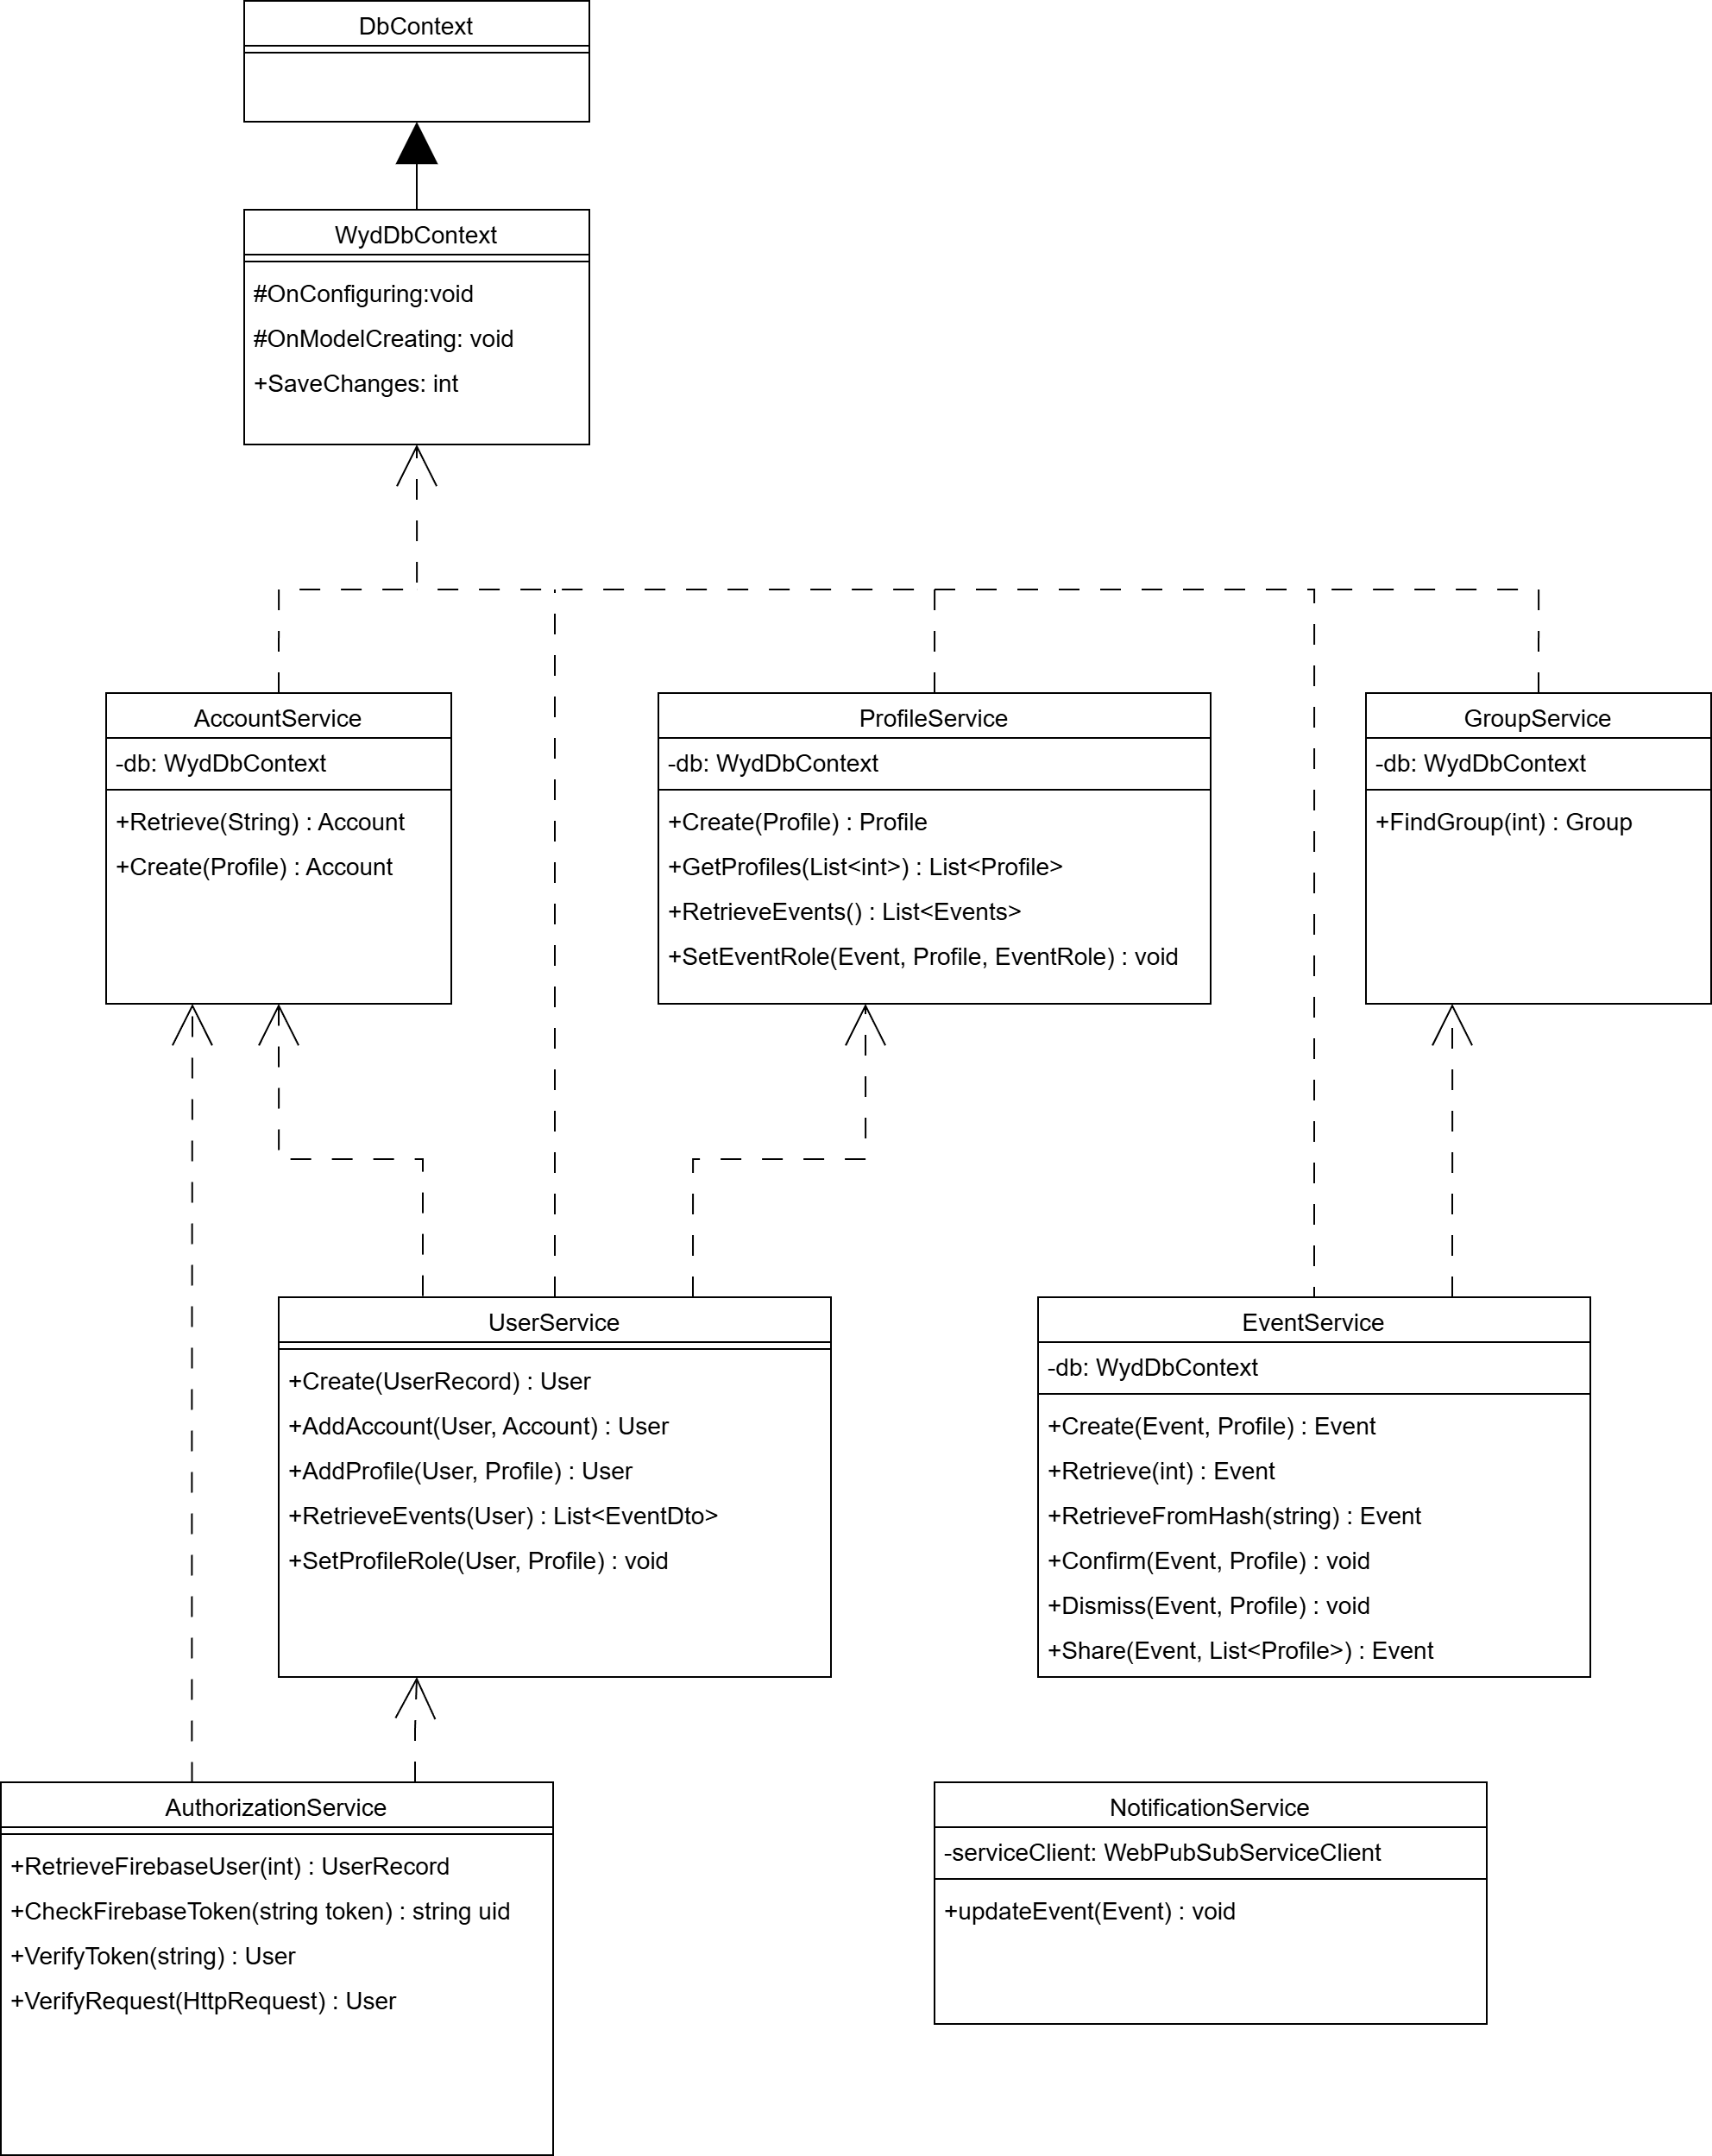
\includegraphics[height=0.8\textheight]{ServiceClassDiagram.png}
        \caption{Modello delle classi del server}
    \end{center}
\end{figure}

Ogni servizio relativo alla manipolazione degli elementi del dominio
ha bisogno di una connessione con il database
per poter applicare le modifiche desiderate.
Questa viene implementata da una classe dedicata chiamata WydDbService.
WydDbService racchiude la logica
e le impostazioni legate alla persistenza principale.
Si concentrano così in un unico luogo tutte le necessità e
le configurazioni di basso livello relative alla sua interazione,
quali la definizione del dominio e delle sue relazioni,
ma anche le proprietà degli indici e le varie operazioni,
dal recupero ad altre più particolari.
L'implementazione delle classi del dominio viene trattata nei capitoli seguenti.\\
\\
Per alcuni compiti specifici sono state implementate classi apposite.
In particolare, 
AuthorizationService si occupa dell'autenticazione e dell'autorizzazione della richiesta,
mentre NotificationService astrae la relazione 
con il servizio di aggiornamento in tempo reale.\\
\\
La maggior parte delle funzioni hanno il compito di rispondere a una richiesta REST,
in cui l'utente cerca di recuperare dei dati o di modificarli.
Ogni funzione di questo tipo seguirà in generale lo stesso procedimento.
Il primo passo consiste nell'autenticare l'utente che fa la richiesta,
analizzando il relativo token.
Si controlla poi che l'utente abbia i permessi necessari
per eseguire l'operazione desiderata.
Se è tutto in regola, si procede a elaborare i dati di ingresso
tramutandoli, se necessario, in oggetti logici.
Si procede quindi con l'esecuzione voluta, la vera responsabilità della funzione.
In base alla natura dell'operazione,
potrebbe essere opportuno aggiungere messaggi in coda per invocare altre funzioni,
quali quelle responsabili per l'invio di notifiche agli utenti coinvolti.
Infine, si restituisce la risposta dell'operazione avvenuta a buon fine,
con in allegato i dati eventualmente necessari.
Tutto il processo viene inserito in un blocco che 
permette l'identificazione di errori e la gestione della relativa risposta.\\
\\
Per allineare i dati a disposizione del server con il dominio del client
e per ridurre l'invio delle informazioni non necessarie, sono stati creati dei Data Transfer Object(DTO).
I DTO sono classi logiche che prevedono almeno un costruttore che, dato l'elemento del dominio,
ne copia solo le informazioni necessarie.
Questo permette di creare rappresentazioni dei dati come necessarie al client,
mascherando le logiche applicative e di fatto separando le dipendenze del dominio dai requisiti di comunicazione.\\
\begin{figure}[h!]
    \begin{center}
        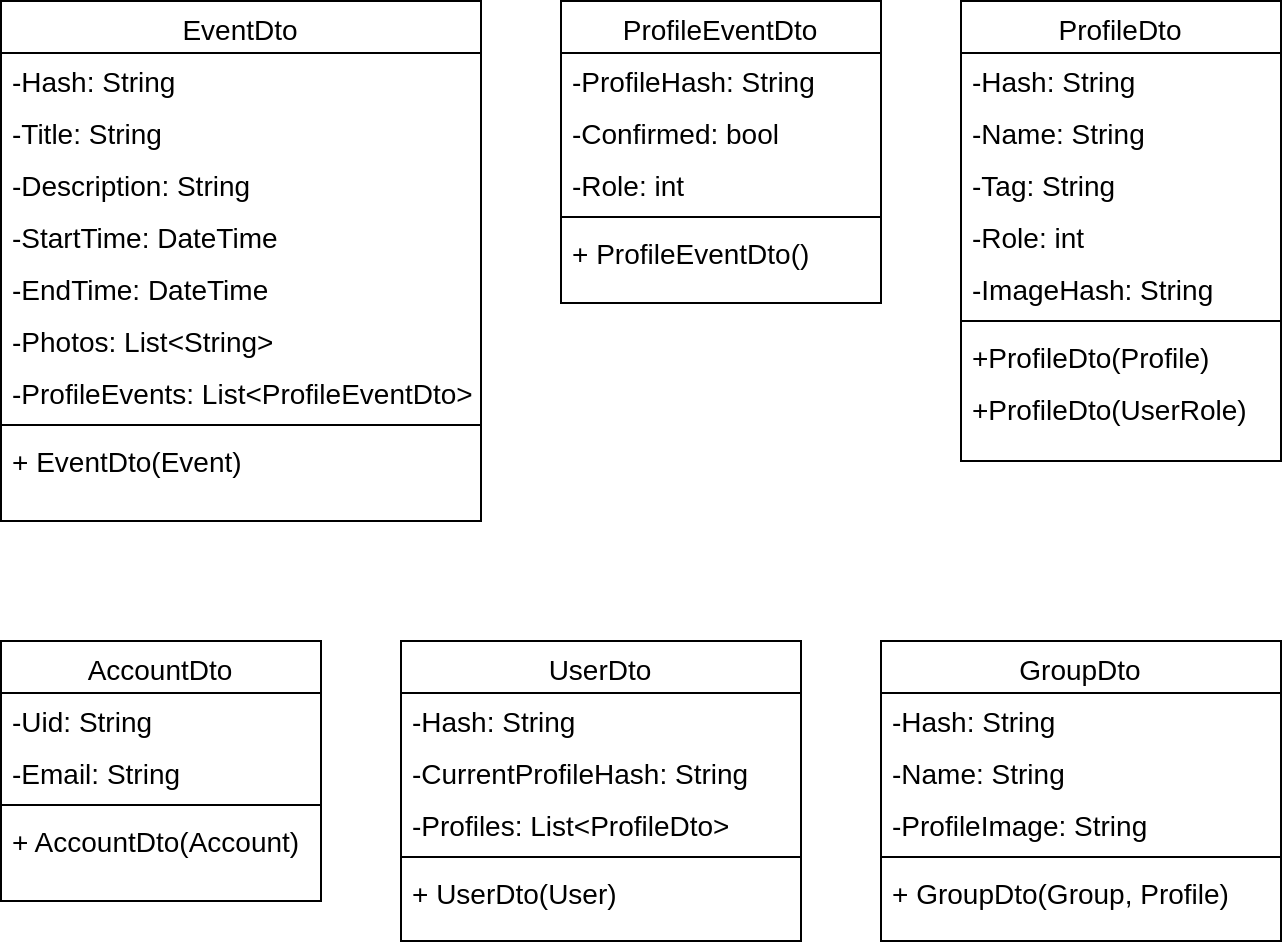
\includegraphics[width=\textwidth]{DTOClassDiagram.png}
        \caption{Modello delle classi dei data tranfer object}
    \end{center}
\end{figure}
\\
Per ogni metodo pubblico delle classi service sono stati implementati dei test.
I test permettono la simulazione di differenti situazioni
per controllare che il codice segua il comportamento desiderato.
La loro implementazione è quindi precedente allo sviluppo stesso delle classi,
in quanto le aspettative sono già note, e il superamento dei test determina la correttezza del metodo.
Inoltre, in caso di necessità particolari che escono dalle normali aspettative della funzione,
quali, ad esempio, il controllo di un valore particolare o l'implementazione di un vincolo specifico,
i test assicurano la loro futura presa in carico anche in caso di modifica totale del codice.\\
\begin{figure}[h!]
    \begin{center}
        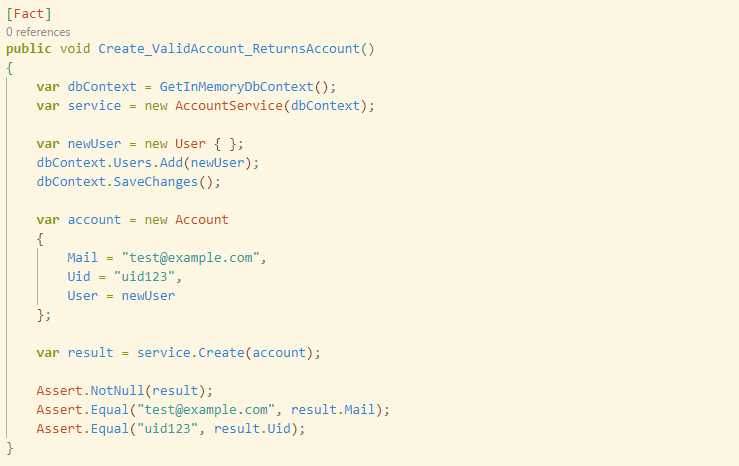
\includegraphics[height=.35\textheight]{TestAccount2.png}
        \caption{Test di creazione di un account}
    \end{center}
\end{figure}

\clearpage




%
\section{Autenticare le richieste: la scelta del servizio e la sua integrazione}


Poiché la modalità di autenticazione rappresenta
un elemento importante per l'esperienza utente,
in quanto deve assicurare un accesso sicuro all'applicazione mantenendone la semplicità,
la facilità del processo di autenticazione deve essere garantita.
L'applicazione deve consentire la possibilità di registrarsi creando un nuovo account dedicato,
ma è altrettanto essenziale che permetta agli utenti di farlo anche
tramite il proprio servizio di autenticazione preferito,
migliorando sicuramente l'usabilità e l'apprezzamento.
Di conseguenza, il sistema di gestione degli accessi deve supportare
sia la registrazione e la gestione autonoma degli account specifici per il servizio,
sia fornire l'integrazione con provider di autenticazione esterni.\\
\\
Per lo scopo, Azure fornisce Microsoft Entra ID,
parte della suite di servizi di autenticazione e autorizzazione Microsoft Entra.
Sebbene teoricamente in grado di soddisfare i requisiti sopra indicati,
la complessità della documentazione e le difficoltà riscontrate nell'integrazione con il servizio dell’applicativo
hanno portato a valutare soluzioni alternative negli ambienti cloud.\\
\\
\begin{wrapfigure}{r}{0.25\textwidth}
    \centering
    
\includegraphics[height=.12\textheight]{firebase.png}
    Firebase Authentication
\end{wrapfigure}
La scelta è quindi ricaduta su Firebase Authentication,
il servizio di autenticazione di Google Cloud Provider,
che garantisce sia la possibilità di creare account dedicati
che di collegarsi attraverso altri servizi di autenticazione.
Presenta librerie di integrazione sia tramite Flutter che tramite C\#
che risultano facili da utilizzare,
oltre a fornire una piattaforma di gestione con un'interfaccia chiara e intuitiva.
Dal punto di vista economico, il servizio risulta vantaggioso,
essendo gratuito fino ai cinquantamila utenti mensili attivi.\\
\clearpage
Firebase si integra facilmente con Flutter,
fornendo una libreria che gestisce completamente l'ottenimento e il mantenimento dei token di autenticazione,
a partire dalle credenziali o dalle verifiche precedenti.
Per ogni richiesta che richiede identificazione un servizio apposito intercetta il messaggio,
recuperando il token e allegandoglielo.
Alla ricezione del messaggio, il server estrae il token dalla richiesta,
per poi contattare Firebase grazie l'astrazione fornita dalla libreria.
Firebase controlla il token e, se corretto,
ne restituisce i dati dell'account relativo.\\
\begin{figure}[htpb]
    \centering
    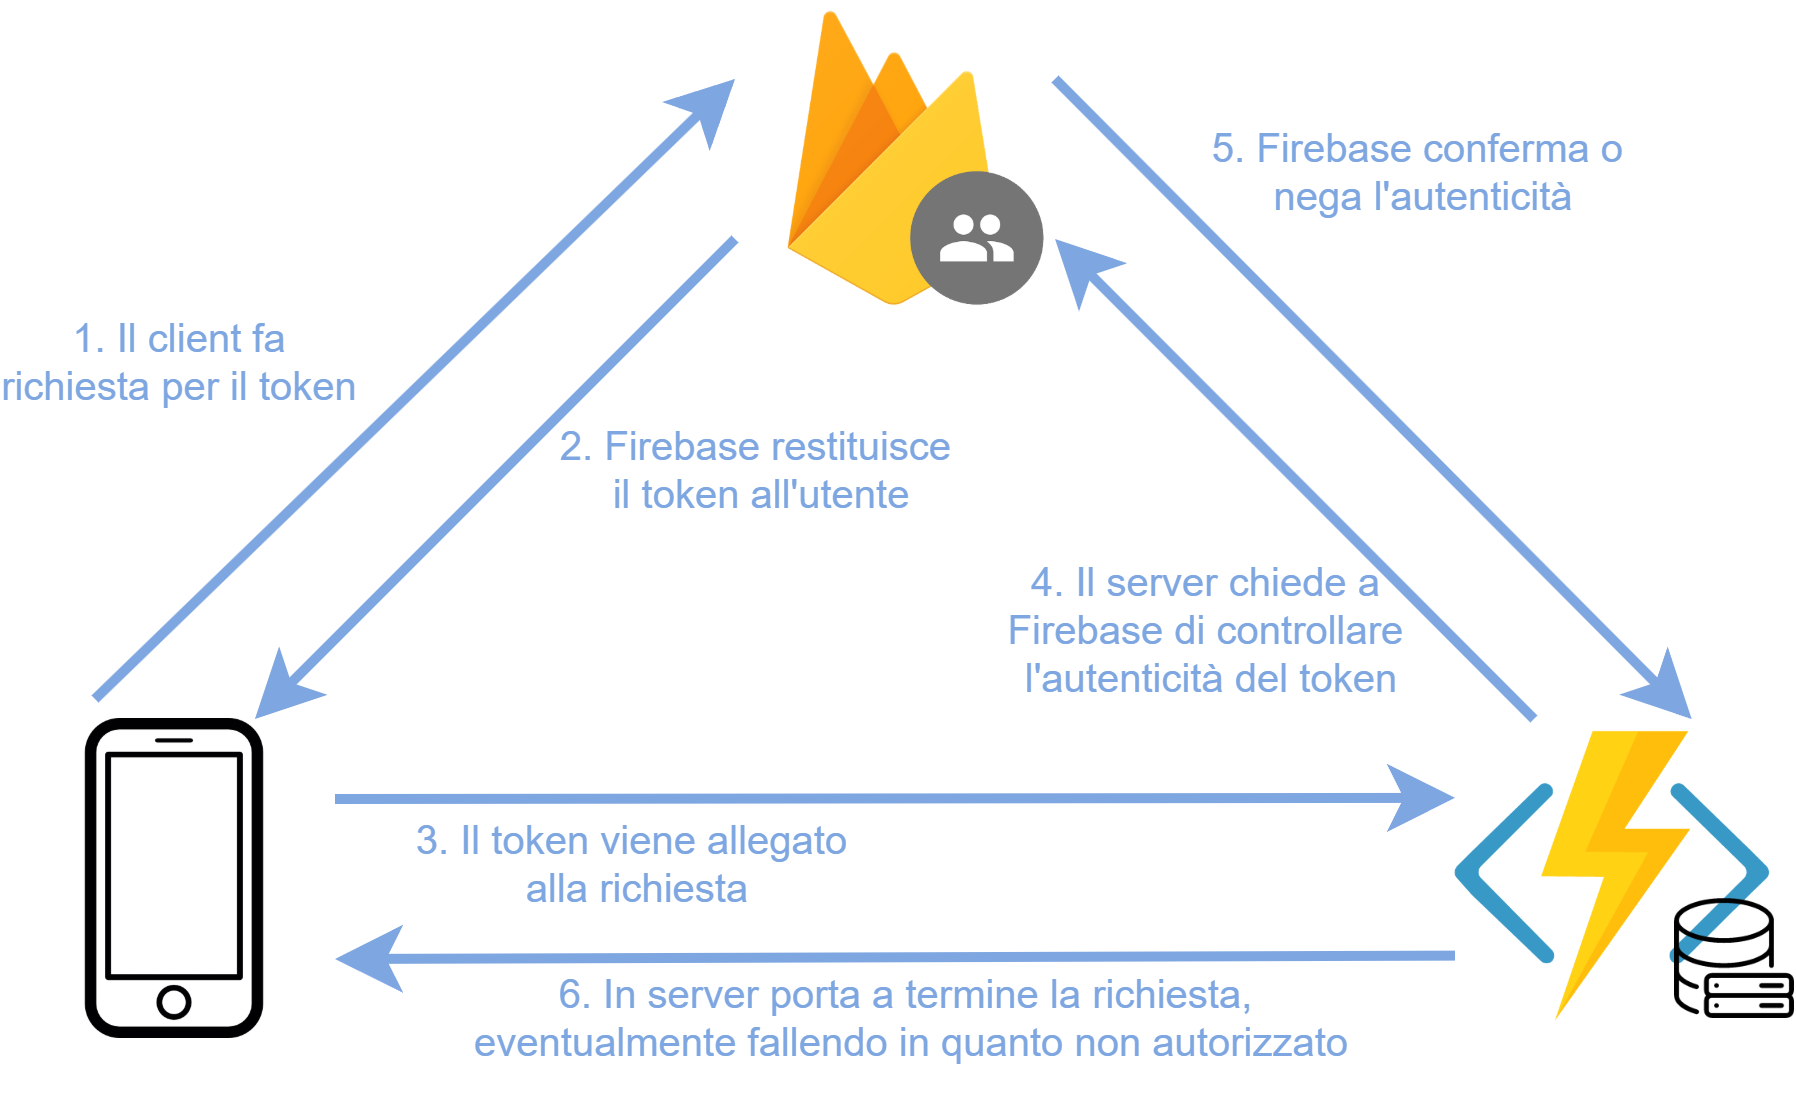
\includegraphics[width=\textwidth]{TokenLogin.png}
    \caption{Fasi di ottenimento e uso del token}
\end{figure}

Uno dei requisiti del progetto prevede
che ogni account sia associato in modo univoco a un singolo utente.
Durante la fase di registrazione, tuttavia,
l’account viene inizialmente registrato nel database gestito da Firebase.
Pertanto, al primo accesso, il server, dopo aver verificato l’autenticità della richiesta,
provvede a creare una copia dell’account,
generando poi il relativo nuovo oggetto utente e il primo profilo associato.\\
\\
\begin{figure}[htpb]
    \centering
    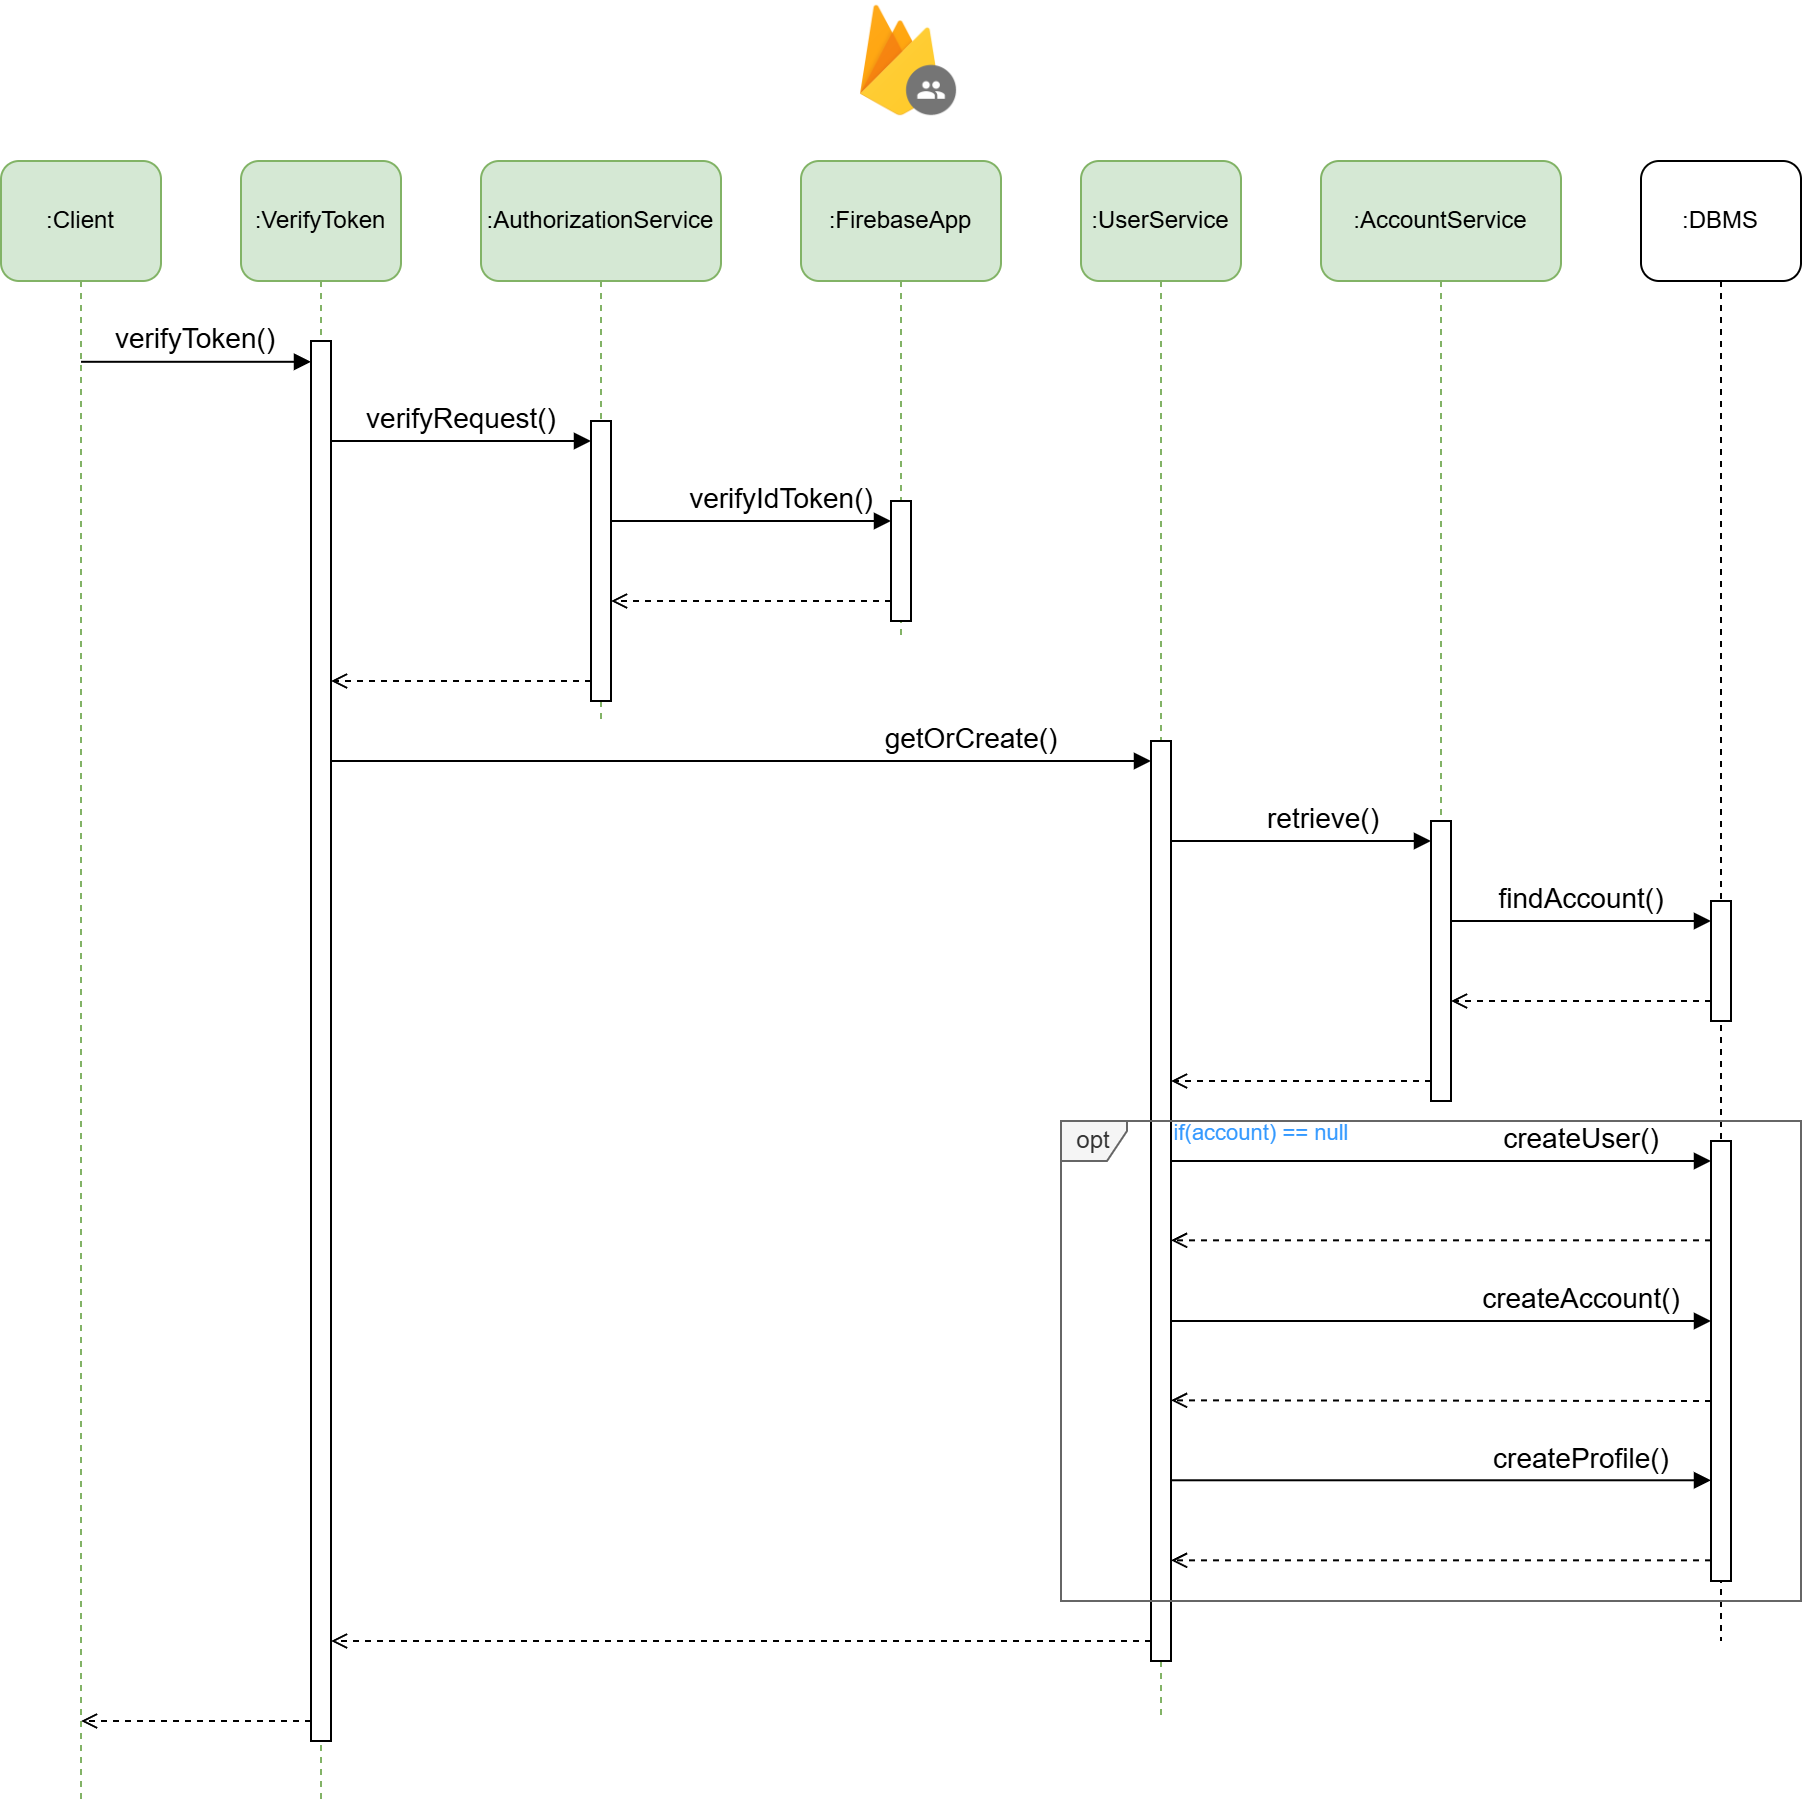
\includegraphics[width=\textwidth]{IIVerifyToken2.png}
    \caption{Diagramma di sequenza per la creazione di un account}
\end{figure}

\clearpage
\section{Uno sguardo sulla sicurezza: segreti e protocolli}
\begin{wrapfigure}{r}{0.25\textwidth}
    \centering
    
\includegraphics[height=.12\textheight]{keyvault.png}
    Azure Key Vault
\end{wrapfigure}
Il collegamento tra i vari componenti all’interno dell’ambiente Azure
richiede l’utilizzo di chiavi e stringhe di connessione.
Il salvataggio di tutte le chiavi sensibili è stato affidato al servizio Azure Key Vault,
un server che permette la centralizzazione dei dati,
cifrando il contenuto e garantendo un controllo maggiore sul loro utilizzo. \\
Quando necessario i servizi, in particolare le Azure Functions,
contatteranno il Key Vault per l'ottenimento delle chiavi necessarie,
separando di fatto la logica implementativa dai segreti necessari per la sua esecuzione,
riducendo così il rischio di una perdita delle chiavi derivata da un errore dello sviluppo.\\
\\
Le comunicazioni tra i vari componenti devono avvenire in sicurezza,
garantendo autenticità e confidenzialità.
Per questo motivo tutte le comunicazioni tra dispositivi client e
i vari servizi utilizzano la tecnologia TLS,
che permette di cifrare i messaggi grazie a uno standard collaudato.
In particolare, le comunicazioni tra i client e Azure Functions,
così come con Firebase Authentication e il server per la persistenza delle immagini,
avvengono tramite protocollo HTTPS,
mentre le comunicazioni con il server per gli aggiornamenti in tempo reale usano il protocollo WSS.\\
\\
Il rischio di saturazione delle risorse viene mitigato
aggiungendo un duplice controllo sulle dimensioni delle richieste.
In primo luogo si limita la dimensione massima della singola richiesta,
facendo particolare attenzione alle richieste che contengono immagini,
controllandola sia nel momento dell'invio che nel momento della ricezione.
Inoltre, alla fine di ogni richiesta più grande di una determinata soglia,
la dimensione viene sommata alle precedenti nell'ultimo periodo e,
se la somma risulta troppo elevata, viene limitato l'utilizzo per quell'utente.\\
\\
Per evitare un numero eccessivo di richieste totali,
che possono provocare anch'esse una riduzione del servizio,
è possibile integrare nel sistema risorse create appositamente da Azure,
quali Azure DDOS Protection.\\
\\
L’accesso al database è ristretto alle sole risorse Azure,
garantendo l’isolamento dall’esterno,
che comprometterebbe altrimenti l’affidabilità dei dati.\\
\\
Infine, l’identificativo di ogni elemento del dominio è nascosto all’utente
tramite la creazione di codici hash univoci
che permettono comunque l'identificazione dell'oggetto senza rivelare ulteriori informazioni.
In particolare, il recupero delle immagini (disponibili in teoria pubblicamente),
avviene grazie a un link univoco dato dalla combinazione degli identificativi dell'evento e dell'immagine.
Utilizzando i codici di hash diventa molto complicato ritrovare le immagini
senza essere a conoscenza dei codici,
che non avendo natura incrementale ma distribuita rende
indovinare l'unica strategia per trovare un link valido.


\section{Il monitoraggio dei servizi}

Il monitoraggio del sistema è attuato in due modalità:
tramite il salvataggio dei log e grazie al controllo delle prestazioni del sistema.\\
\\
Relativamente a Firebase Authentication vengono forniti inclusi al servizio
sia le interfacce per il controllo delle prestazioni che per la gestione dei log.
Non è quindi richiesta alcuna ulteriore azione.\\
\begin{wrapfigure}{r}{0.25\textwidth}
    \centering
    
\includegraphics[height=.12\textheight]{insights.png}
    Azure Application Insights
\end{wrapfigure}
Per monitorare le Azure Functions sarà invece necessario
affiancargli un'istanza di Azure Application Insights,
servizio nato appositamente per controllare il funzionamento e la risposta dei servizi Azure.
Una volta collegato il servizio, infatti,
Application Insight permette la presentazione e l'analisi di numerose metriche,
quali il tempo di risposta e il consumo di risorse.
Consente inoltre di testare la risposta dell'applicativo
simulando diversi scenari e riassumendo il loro comportamento.\\
\\
La creazione dei log è invece delegata al programmatore,
in quanto è necessario integrarli nel codice.
Nel momento della creazione, ogni funzione riceve, tramite dependency injection,
un servizio Logger che permette la creazione e il salvataggio dei log.
La funzione non dovrà fare altro che chiamare il metodo apposito per generare e salvare un log.
Tali log saranno poi consultabili e analizzabili tramite l’interfaccia fornita da Azure Application Insight.\\
\clearpage
\chapter{La gestione della persistenza}

Nel contesto di un sistema che prevede la gestione di eventi e impegni,
è essenziale garantire all’utente di poter accedere in qualsiasi momento alla propria agenda,
visualizzando gli appuntamenti più urgenti e pianificando efficacemente il proprio tempo.
Deve perciò essere possibile trovare e mostrare nel minor tempo possibile i dati relativi all’agenda.
Per soddisfare questo requisito,
il recupero e la visualizzazione dei dati devono avvenire con la massima rapidità possibile,
riducendo i tempi di latenza e ottimizzando il flusso di interazione con l’interfaccia utente.\\
\\
L'adozione di un meccanismo di salvataggio locale sui dispositivi
offre il vantaggio di migliorare le prestazioni,
consentendo un accesso immediato alle informazioni senza dover effettuare continue richieste al server remoto.
Tuttavia questa soluzione rimane parziale,
in quanto non garantisce una persistenza a lungo termine dei dati,
né assicura la loro disponibilità in ogni momento,
per essere in grado di sincronizzare più dispositivi.
Per superare tali criticità,
è necessario definire una strategia di gestione della memoria
che preveda una fonte di dati centrale e autorevole,
alla quale tutti i dispositivi possano fare riferimento per recuperare e
aggiornare le informazioni in modo coerente e affidabile.\\
\\
Un sistema di persistenza efficace deve quindi prevedere
un meccanismo di sincronizzazione tra i dati salvati localmente e
la loro controparte ufficiale memorizzata nel database principale.
Questo processo deve essere progettato in modo da garantire
integrità, coerenza e scalabilità nelle interazioni,
per essere resistente anche in presenza di un volume significativo di richieste concorrenti.
La struttura del sistema di memorizzazione deve inoltre essere progettata
tenendo conto del dominio applicativo e delle esigenze specifiche di utilizzo,
al fine di assicurare un bilanciamento ottimale tra efficienza e robustezza operativa.\\
\\
Oltre alla gestione della persistenza dei dati per il singolo utente,
è necessario affrontare il problema della modifica di eventi condivisi.
Poiché l'applicazione consente a più utenti di interagire sugli stessi eventi,
le modifiche effettuate da un partecipante devono essere propagate
in tempo reale agli altri dispositivi coinvolti.
Questo introduce la necessità di implementare un sistema di aggiornamento distribuito,
in grado di mantenere sincronizzati non solo i dispositivi di un singolo utente,
ma anche quelli di tutti gli utenti interessati dalle modifiche.\\
\\
La gestione dell’accesso ai dati richiede quindi l’implementazione di un’architettura che preveda
un punto di riferimento centrale chiaro e affidabile,
capace di fungere da fonte primaria delle informazioni.
Al tempo stesso, l’utilizzo di copie locali dei dati sui dispositivi client
consente di ridurre l’impatto delle latenze di rete,
migliorando la reattività dell’interfaccia e offrendo un’esperienza utente più fluida.
Tuttavia, questa scelta introduce la necessità di gestire due livelli distinti di responsabilità:
da un lato, il client deve occuparsi di mantenere aggiornati i dati memorizzati localmente,
mentre il server deve garantire la corretta distribuzione delle modifiche agli altri dispositivi interessati.
La sincronizzazione e la gestione delle versioni dei dati diventano quindi
elementi chiave per assicurare la coerenza del sistema e
prevenire eventuali conflitti tra modifiche concorrenti.

\clearpage
\section{L'analisi per l'identificazione del database}

Nell’implementazione di applicazioni scalabili, la gestione del salvataggio dei dati
può essere strutturata secondo un modello centralizzato o distribuito,
a seconda delle esigenze di affidabilità, scalabilità e prestazioni del sistema.
L’adozione di un’architettura di memoria distribuita offre molteplici vantaggi,
tra cui una maggiore resilienza ai guasti di una singola fonte,
la riduzione del carico di memoria su un'unica risorsa di archiviazione e
una migliore scalabilità complessiva del sistema.
Tuttavia, questa soluzione introduce una maggiore complessità infrastrutturale,
poiché richiede meccanismi avanzati per garantire il recupero,
l'affidabilità e la consistenza delle informazioni.\\
\\
Salvo specifici requisiti che rendano indispensabile la distribuzione totale o parziale della memoria,
una strategia basata su un database centralizzato risulta più efficiente
dal punto di vista prestazionale e semplifica la gestione complessiva del sistema.
L’adozione di un’architettura centralizzata consente infatti
di ottimizzare i tempi di accesso ai dati e ridurre la latenza delle operazioni,
grazie a una minore complessità di sincronizzazione e
di mantenimento della consistenza delle informazioni.\\
\\
I database non distribuiti si suddividono in due macro categorie principali: relazionali e non relazionali.\\
I database relazionali si caratterizzano per strutture dati rigide e schematizzate,
che consentono di stabilire connessioni tra le diverse entità in tempi estremamente rapidi,
garantendo allo stesso tempo operazioni atomiche.
Viceversa, i database non relazionali offrono una maggiore flessibilità strutturale,
permettendo l’archiviazione di dati eterogenei e adottando un accoppiamento più debole tra i vari oggetti. \\
\\
La scelta della tipologia di database più appropriata dipende direttamente
dalle esigenze specifiche del progetto.
Ogni prodotto è stato infatti realizzato per rispondere a una funzionalità specifica,
introducendo vantaggi per un determinato caso d'uso ma comportando anche punti deboli,
sia in termini di prestazioni che in termini di scalabilità.
Determinare il database più adatto alle esigenze dipende
quindi non solo dalle proprietà intrinseche della tecnologia,
ma sopratutto di come queste riescano a risolvere i particolari problemi che il progetto presenta.
\clearpage

\subsection{Le proprietà dei database relazionali}


I database relazionali gestiscono i dati tramite strutture chiamate schemi.
Lo schema è una struttura rigida i cui campi e le relative proprietà
vengono definite sin dal momento della creazione.
Mantengono però un grande potere espressivo,
in quanto permettono di descrivere direttamente le relazioni(e le loro proprietà) tra gli oggetti,
attraverso la creazione di uno schema dedicato.
Ogni elemento ha un identificativo univoco(Primary Key o PK)
attraverso cui viene individuato all'interno del suo schema.
Se lo schema descrive una relazione, viene identificato tramite
una combinazione di identificativi derivati(Foreign Key o FK).
Gli aggiornamenti agli schemi avvengono tramite un rigoroso sistema di transazioni.
La transazione è il processo attraverso il quale una modifica viene portata a termine,
a cui viene riservata per il tempo necessario la risorsa interessata.\\
\\
Grazie alla struttura statica dei dati, unitamente alle relazioni predefinite del dominio,
il tempo di recupero e analisi dei dati risulta altamente ottimizzato.
L'utilizzo delle primary e foreign key consente al database di creare automaticamente indici
dedicati che consentono l'individuazione di un oggetto in tempi minimi,
e facilitano l'incrocio delle informazioni contenute all'interno delle relazioni.
L'utilizzo delle transazioni rende i database relazionali in grado di garantire
le proprietà di Atomicità, Consistenza, Isolamento e Durabilità (ACID),
assicurando un’elevata affidabilità dei dati.\\
\\
La rigidità del modello non permette però di avere un elemento
di uno schema che presenti proprietà diverse da tutti gli altri.
Non è quindi supportata l'aggiunta o la modifica di campi all'interno di un oggetto,
a meno di non cambiare la definizione dell'intero schema.
L'utilizzo delle transazioni introduce inoltre la necessità, durante le operazioni di scrittura,
di bloccare temporaneamente le risorse interessate,facendo fallire o aspettare altre richieste simultanee sullo stesso elemento,
potenzialmente influenzando le prestazioni complessive del sistema.\\
\\
Per poter garantire il successo di una transazione
il database deve controllare tutte le sessioni con il server,
il che comporta una limitazione al numero massimo di connessioni(e quindi richieste) contemporanee possibili.
Inoltre gli indici dipendono da tutti gli elementi del database,
e allo stesso modo gli schemi delle relazioni sono
fortemente accoppiati con gli schemi delle entità coinvolte.
Risulta quindi arduo dividere degli elementi su più tabelle(sharding),
operazione necessaria per la distribuzione del database su più server,
aumentando di conseguenza la complessità richiesta per essere in grado di scalare orizzontalmente.\\
\\

\subsection {Le proprietà dei database non relazionali}

I database non relazionali, noti anche come NoSQL,
si distinguono per l'adozione di modelli di archiviazione dei dati flessibili,
che si discostano dalla rigida struttura tabellare dei database relazionali.
Questi modelli includono approcci chiave-valore, documento, colonnare e a grafo,
ciascuno ottimizzato per specifiche esigenze applicative,
come la gestione di file, dati semi-strutturati, o la rappresentazione di relazioni complesse.\\
\\
La loro caratteristica fondamentale è la capacità di salvare le informazioni in forme variabili,
permettendo di modificare la struttura dei dati senza la necessità di riconfigurare lo schema del database.
La vera forza dei database NoSQL, tuttavia, risiede nella loro predisposizione alla scalabilità orizzontale.
I NoSQL sono infatti progettati per distribuire il carico su più server,
consentendo di gestire volumi crescenti di dati e richieste semplicemente aggiungendo nuovi nodi al sistema.\\
\\
Nonostante i vantaggi in termini di scalabilità,
i database non relazionali presentano però alcune limitazioni significative.
La più rilevante è la rinuncia alle proprietà ACID, alla quale si contrappone,
per favorire la disponibilità e la tolleranza ai partizionamenti,
una consistenza finale (eventual consistency),
dove le modifiche ai dati si propagano attraverso il sistema in un certo lasso di tempo,
piuttosto che essere immediatamente consistenti su tutti i nodi.
Questo può portare a letture di dati non aggiornati in determinate circostanze,
il che può essere un problema per applicazioni che richiedono forte consistenza,
ma che deve essere comunque tenuto in considerazione durante l'analisi,
per progettare un'applicazione che sia resistente a un asincronismo temporaneo dei dati.\\
\\



%    Per mitigare queste limitazione alcuni database offrono strategie di strong consistency,
%    indici?
%   accostamento di databases?


\subsection{L'impatto delle relazioni delle entità sulle prestazioni}

L'aspetto determinante alla base della scelta del database
riguarda la gestione delle relazioni tra le entità.
È fondamentale analizzare la distribuzione delle richieste per ciascun elemento
e il carico computazionale che ogni operazione comporta.
Tra le operazioni più costose in termini di prestazioni,
che più ostacola e rallenta il recupero dei dati, vi è l'operazione di unione(join).
Durante l'operazione di unione vengono incrociati i dati di vari elementi
per restituire un oggetto coerente che presenti tutte le proprietà necessarie,
originariamente distribuite in molteplici tabelle. \\
\\
Nonostante l'esecuzione di join su database sia altamente ottimizzata
(particolarmente in quelli relazionali) e facilitata dall'utilizzo di indici,
introduce comunque carichi computazionali di grande entità che impattano
significativamente sui tempi di risposta delle richieste,
crescendo proporzionalmente con la quantità dei dati presenti nel database.
Per questo motivo è bene modellare il dominio nell'ottica di ridurre il più possibile
le richieste che comportano l'incrocio di dati da tabelle diverse.\\
\\
Le relazioni tra elementi possono essere classificate in tre categorie principali:
di tipo uno a uno, uno a molti, e molti a molti. \\
Nelle relazioni uno a uno il recupero dei dati è diretto
e richiede uno sforzo computazionale limitato.
Nei casi uno a molti e molti a molti il reperimento delle informazioni richiede
spesso un'operazione di join, ed è quindi bene eseguire un'attenta valutazione
delle tipologie di accesso per ottimizzarne le prestazioni.
Un'operazione di join è accettabile se il numero delle entità coinvolte è limitato o facilmente reperibile.
Altrimenti, una delle strategie possibili per migliorare l’efficienza delle richieste
offerte dai database non relazionali è la denormalizzazione delle entità.\\
\\
La denormalizzazione consiste nel duplicare o incorporare dati correlati all'interno della stessa entità o documento,
eliminando la necessità di operazioni di join complesse e costose in fase di lettura.
Questo significa che, anziché avere tabelle separate tra due elementi e collegarle tramite chiavi esterne,
un database denormalizzato potrebbe memorizzare direttamente
un array dei dati del primo all'interno del documento del secondo.
Recuperare tutti i dati necessari per una determinata operazione richiede spesso
una singola lettura da un'unica entità, e raramente un'operazione di join,
riducendo drasticamente il numero di accessi al disco e le elaborazioni computazionali.
Questo è particolarmente vantaggioso in scenari
dove le operazioni di lettura sono molto più frequenti di quelle di scrittura.\\
\\
Per ogni dato duplicato, infatti, si introduce la complessità
di dover garantire la coerenza di tali dati attraverso il sistema.
Se un'informazione duplicata viene modificata in una delle sue occorrenze,
è essenziale che tale modifica si propaghi correttamente a tutte le altre copie
per evitare che il database contenga dati incoerenti.
Non esiste un meccanismo automatico che ne assicura la coerenza,
e la sua creazione può diventare onerosa e complessa,
soprattutto in sistemi distribuiti e con elevato volume di scritture.\\
\\
In una relazione uno a molti,
nel caso in cui la richiesta di quell'elemento non sia frequente
ma sia invece importante restituire spesso gli elementi a lui collegati,
conviene copiare gli oggetti relativi all'interno dell'elemento singolo.
L’impostazione inversa, in cui si copia il singolo all’interno dei molti elementi,
comporterebbe l’ispezione di tutti i componenti esistenti alla ricerca di quelli che contengono l’elemento dato.
Se però, viceversa, sono frequenti le richieste relative agli elementi multipli, e la loro relazione è importante,
conviene copiare il singolo all'interno di detti elementi, per evitarne il recupero ogni volta.\\
\\
Nel caso molti a molti bisogna considerare ancora di più la proporzione delle richieste.
Le relazioni molti a molti vengono generalmente descritte da un terzo oggetto,
che oltre a mantenere i riferimenti alle due entità,
descrive le proprietà della relazione.
Le scelte principali che si possono fare in questo caso sono due.
Se la lettura è sbilanciata verso uno dei due elementi della relazione,
e, allo stesso tempo, è importante che vengano restituiti gli oggetti
che descrivono l'associazione assieme all'elemento stesso,
è bene integrare le associazioni in quell'elemento.
Altrimenti, in caso la necessità di lettura sia equiparabile da entrambe le parti,
è necessario mantenere l'associazione come documento indipendente,
eventualmente copiando i dati richiesti per evitare
di dover recuperare il terzo elemento della relazione.
\clearpage


\subsection{Analisi del dominio}

Il dominio descrive i componenti dell'applicazione e le loro relazioni.
Ne vengono espresse le dipendenze, i rapporti reciproci e la cardinalità delle relazioni.
La sua analisi, integrata con la previsione del carico delle richieste,
permette di fornire un quadro dettagliato sulle necessità relative,
per poter poi definire la tipologia delle strutture in cui salvare i dati e
le caratteristiche richieste al database.\\

\begin{figure}[htpb]
    \centering
    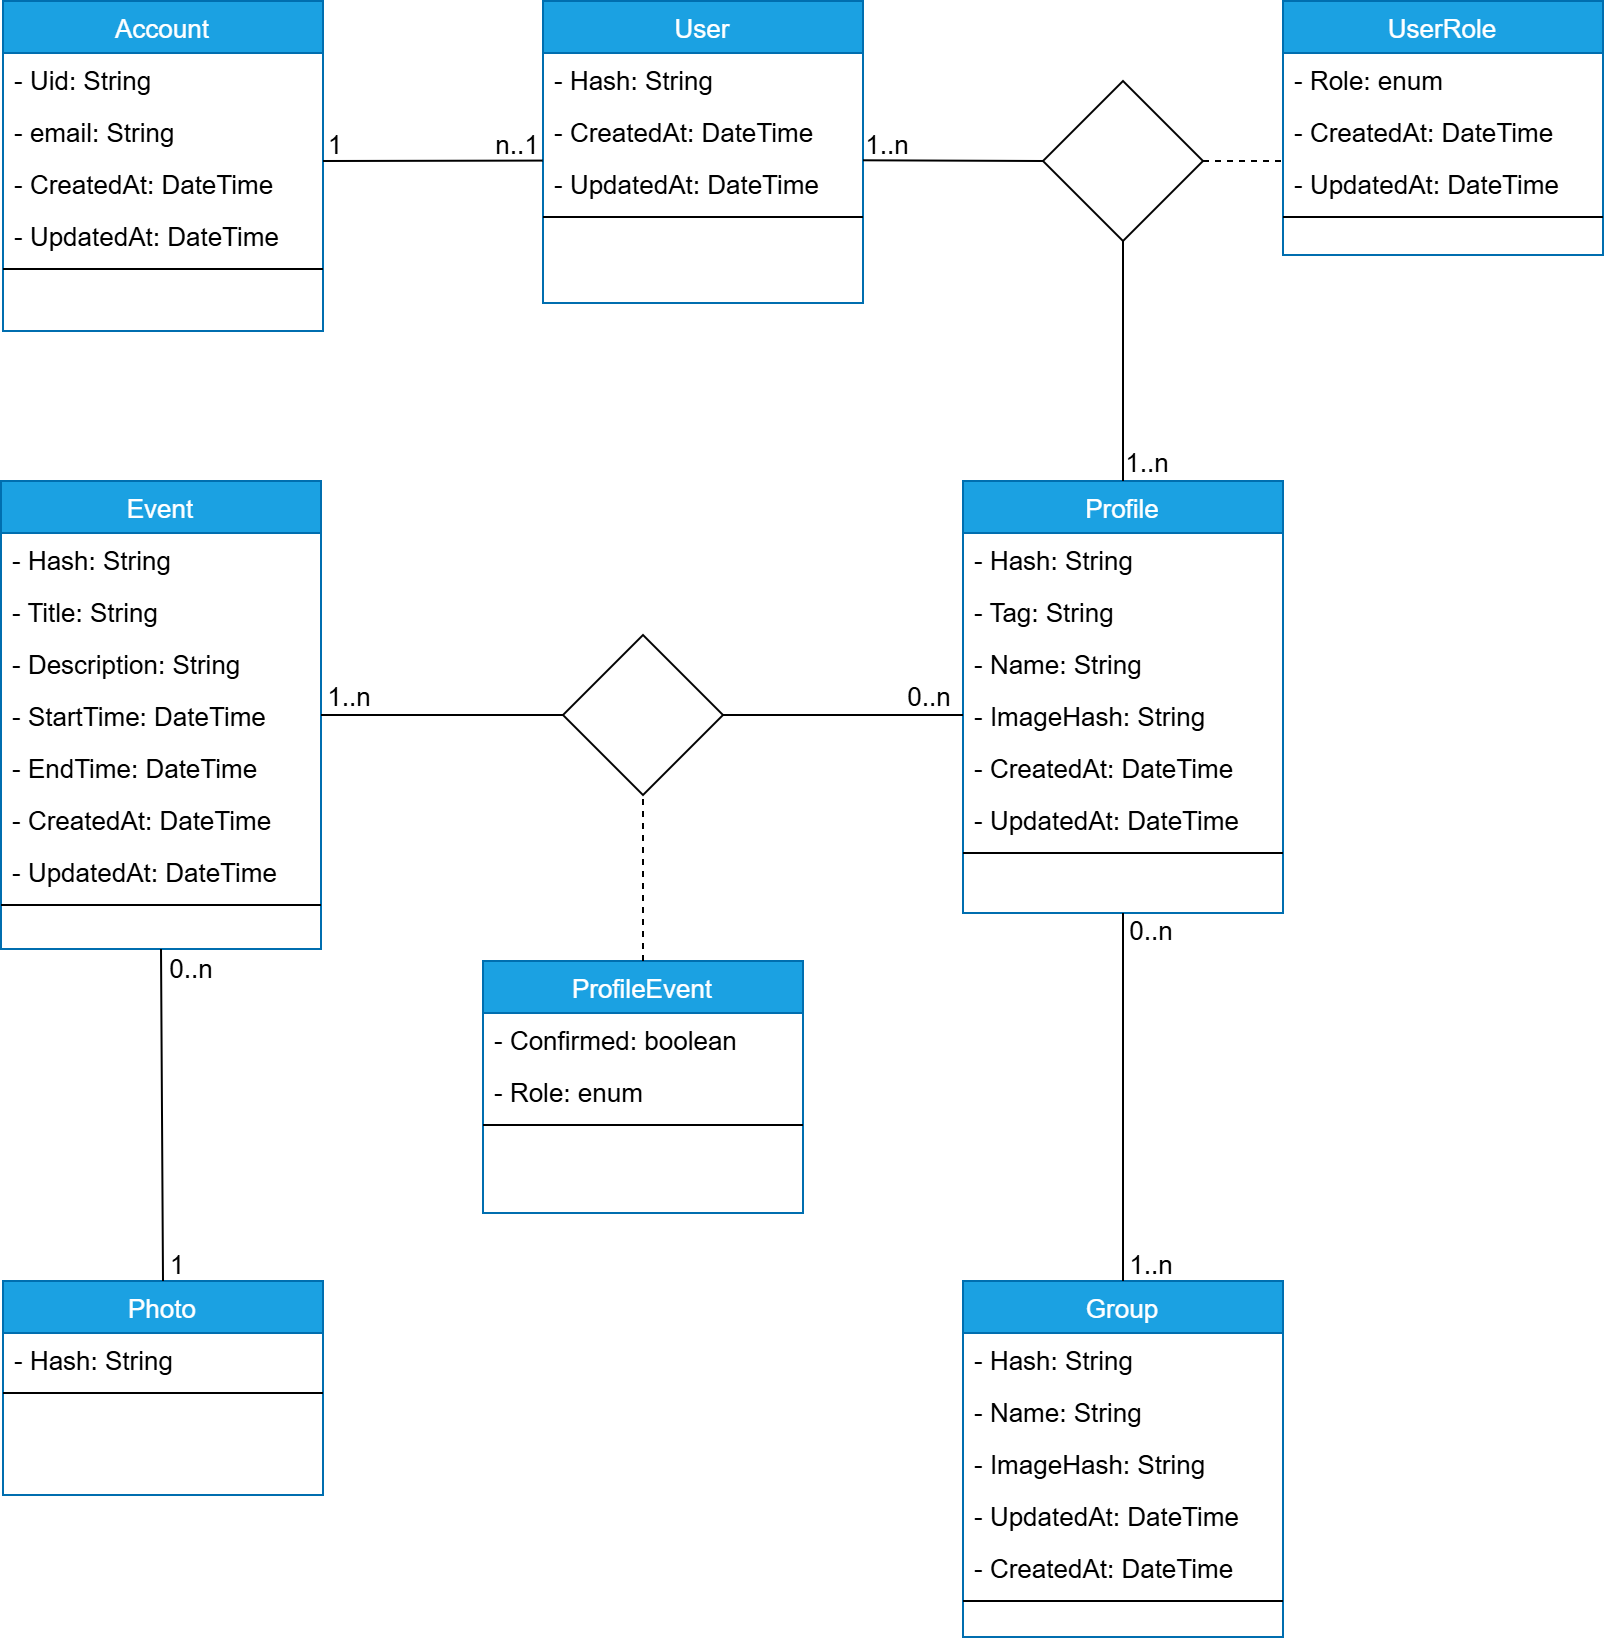
\includegraphics[width=\textwidth]{ProgettoDominioServer.png}
    \caption{Diagramma del dominio di Wyd}
\end{figure}

\clearpage
Le entità Account, User e Profile, assieme alla relazione UserRole,
descrivono le specifiche di autenticazione, identificazione dell'utente e i suoi ruoli sui profili associati.
I loro dati vengono recuperati solamente una volta nel ciclo di vita del programma,
a seguito del login dell'utente.
Vengono poi salvati in memoria locale,
riducendo il numero di richieste relative successive a un controllo su eventuali aggiornamenti.
Si prevede che le modifiche a questi elementi siano sporadiche.\\
Allo stesso modo gli oggetti Group vengono recuperati solo all'avvio dell'applicazione, e,
salvo rari aggiornamenti, non comportano ulteriori richieste.
Le richieste di lettura e scrittura previste per questi elementi sono quindi in quantità esigua,
e influiscono secondariamente sulle performance del sistema.\\
\\
La maggioranza delle richieste verterà sull'ottenimento dei dati relativi agli Event e ai Profile.
Gli Event descrivono gli impegni ai quali i profili partecipano.
Essendo la loro relazione di tipologia molti a molti,
si introduce l'entità ProfileEvent che descrive l'associazione evento-profilo,
indicando che un evento è condiviso con un profilo.
La proprietà più importante di ProfileEvent è sicuramente Confirmed,
una variabile booleana che esprime la partecipazione o meno di un profilo all'evento.
È ragionevole prevedere che la cardinalità dei profili associati a un evento non superi l'ordine delle centinaia.
Agli eventi che si associano ai profili l'ordine di grandezza invece previsto risiede nelle migliaia.
Ci sono molteplici situazioni da tenere in considerazione analizzando questa relazione.\\
\\
Sicuramente bisogna considerare il recupero specifico delle entità Event e Profile.
Questo accade quando un utente decide di entrare nel dettaglio di uno dei due elementi,
comportando la richiesta di tutti i dati dell'oggetto.
Consistono in un'operazione di lettura tutto sommato semplice:
essendo l'utente in possesso dell'identificativo dell'elemento,
la ricerca risulta diretta, e i dati da recuperare esigui.\\
\\
La conferma o la disdetta a un evento vede la modifica di un ProfileEvent.
Questa operazioni di per sé risulta veloce
in quanto necessita di recuperare un solo elemento per poi modificarlo.
Allo stesso modo la modifica di un evento comporta l'aggiornamento di un solo oggetto Event,
a seguito però del recupero del ProfileEvent associato,
necessario per controllare i permessi del profilo sull'evento.
Entrambe le operazioni richiedono però l'invio di una notifica verso tutti i profili interessati,
che necessita il recupero di tutti i ProfileEvent associati ogni volta che una di queste accade.\\
\\
La probabilità che un evento o un qualunque ProfileEvent a esso associato
venga modificato risulta quindi complessivamente elevata e, di conseguenza,
l'operazione di recupero degli identificativi di tutti i profili associati all'evento
è da considerarsi frequente.
Questa operazione, in base all'implementazione, può risultare costosa:
una separazione, un accoppiamento debole o la mancanza di indici tra Event e ProfileEvent
determinano la necessità di ricercare le entità in tutto il database.\\
\\
Quando un utente accede per la prima volta su un dispositivo
è necessario ottenere gli eventi associati ai suoi profili.
Allo stesso modo, a ogni avvio dell'applicazione si recuperano gli eventi
che hanno subito modifiche dall'ultimo accesso.
Inoltre, per poter garantire(all'interno di un determinato vincolo temporale)
la consistenza dei dati anche a livello locale,
il client applica una strategia di long polling
per ottenere gli eventi che sono stati modificati dall'ultimo aggiornamento noto.
L'operazione di ritrovamento degli eventi a partire dal profilo risulta quindi centrale e frequente,
per quanto possa accettare un tempo di esecuzione leggermente più lungo. \\

\begin{longtable}{|P{9.5cm}|P{2.5cm}|P{2.5cm}|}
    \hline
    \textbf{Funzionalità}                           & \textbf{Frequenza } & \textbf{Complessità} \\
    \hline
    Recupero di un Event                            & Media               & Semplice             \\
    \hline
    Recupero di un Profile                          & Media               & Semplice             \\
    \hline
    Modifica di un Event                            & Media               & Semplice             \\
    \hline
    Conferma/disdedda di un Event                   & Alta                & Semplice             \\
    \hline
    Ritrovamento dei Profile associati a un Event   & Alta                & Complessa            \\
    \hline
    Ritrovamento degli Event associati a un Profile & Alta                & Complessa            \\
    \hline
    \caption{Funzionalità principali tra Event e Profile}
\end{longtable}

La relazione tra Event e Photo impatta sulle prestazioni del sistema solo in casi particolari e
verrà affrontato nei capitoli successivi.
\clearpage
%\section{L'implementazione del database}
Nelle sezioni precedenti si è discusso delle proprietà
offerte dai diversi tipi di database e
delle necessità che il dominio impone sul sistema.
La scelta del database deriva quindi dall'incrocio di tutte queste condizioni,
individuando la tecnologia che meglio riesce a rispondere alle esigenze del progetto.
Ogni tipologia di database comporta un approccio differente alle informazioni,
implicando una strategia di salvataggio e manipolazione dei dati propria.
Le strutture che modellano le entità devono quindi
essere create per sfruttare nella maniera più efficiente possibile
i vantaggi offerti dalla tecnologia scelta.\\
\\
Una volta scelto il database e le strutture in base alla modalità
che più si addicono alle esigenze del progetto,
l'utilizzo di servizi in cloud comporta una maggiore attenzione anche
alle proprietà legate al mantenimento del servizio,
dalle quali derivano le proprietà di scalabilità e affidabilità.
La grande differenza tra i vari servizi sta nelle proprietà del server
incaricato di fornire il potere computazionale necessario per l’esecuzione.
L’architettura del server e la sua integrazione con la tecnologia del database
determinano infatti l’effettiva capacità di scalabilità del servizio.\\
\\
Si intende scalabilità verticale la capacità di aumentare le risorse
della stessa macchina in cui si esegue il codice.
La scalabilità verticale viene definita nel momento di creazione del servizio,
in cui si determinano le risorse da dedicare alla macchina che esegue il programma.
Trattandosi di macchine virtualizzate,
è sempre possibile in un secondo momento aumentare le prestazioni in caso di necessità.\\
\\
Per scalabilità orizzontale si intende invece la capacità di
delegare il carico di lavoro su più macchine, eventualmente coordinando le modifiche.
Questo permette una risposta alle richieste più resistente,
riducendo il rischio di colli di bottiglia che potrebbero venirsi a formare nell’utilizzo di un nodo singolo.
La scalabilità orizzontale richiede però l'implementazione
di tecnologie apposite integrate con il database che permettano l'esecuzione in nodi fisici differenti. \\
\\
Una volta individuata la tecnologia adatta e il livello di scalabilità desiderati,
è bene considerare le altre necessità o le opportunità aggiuntive generate
dalla presenza di un database nel progetto. \\
\\
L’alta disponibilità(HA) è la proprietà di garantire l’accesso al servizio nonostante i guasti.
Ad esempio, si può mantenere una macchina identica al server principale in grado di replicare il servizio,
spostando il carico in caso di guasto del server principale.
Si misura in “numero di nove”, ovvero la quantità di nove presenti
nella percentuale del tempo per il quale si garantisce la disponibilità del servizio.
I servizi offrono diverse qualità di HA, in base alle funzionalità desiderate.\\
\\
Alcuni servizi possono presentare offerte di backup
per riportare il server nello stesso stato di qualche momento precedente.
Questo permette il ripristino del sistema a un punto precedente
rispetto all'avvenimento di eventuali errori o guasti del sistema.\\
\subsection{La scelta del database}

Viste le necessità del progetto in ambito di scalabilità
e le caratteristiche del dominio,
si individua nei database documentali la tecnologia più adatta
per gestire la persistenza centrale dell'applicazione.\\
\\
I database documentali, facenti parte della categoria dei database non relazionali,
rappresentano un paradigma di gestione dei dati
che organizza le informazioni in documenti.
Ogni documento è un'unità autonoma che incapsula la descrizione di un'entità,
contenendo le sue proprietà.
Tali documenti sono logicamente raggruppati in collezioni.
All'interno di una collezione,
ciascun documento è univocamente identificato da un proprio identificativo,
garantendo l'accesso diretto e la manipolazione individuale.\\
\\
Un aspetto distintivo e strategicamente rilevante dei database documentali è
la loro intrinseca capacità di supportare la scalabilità orizzontale in modo nativo.
Data la natura dei documenti e il loro accoppiamento debole con gli altri elementi,
la separazione delle collezioni risulta particolarmente semplificata,
favorendo un partizionamento dei dati,
essenziale per distribuire il database su diversi nodi fisici di archiviazione.
Questo vantaggio è fondamentale in architetture distribuite e ambienti ad alta intensità di dati.\\
\\
Un altro vantaggio derivato dall'utilizzo di un database non relazionale
è la propensione verso la denormalizzazione degli elementi del dominio,
sia strutturale che logica.
La denormalizzazione consiste nel riportare le stesse proprietà degli elementi in più collezioni,
riducendo così, se correttamente ottimizzata,
il numero di join o richieste al database necessario per soddisfare le richieste.
Infatti, vista la riduzione di efficienza nell'incrocio tra entità,
dovuta a una difficoltà intrinseca nell'ottimizzare le join tra documenti,
si propende, invece che a incrociare i dati, a duplicarli sui i vari documenti.
Le operazioni di join sono così agevolate,
in quanto possono essere ottimizzate per
far risiedere la risorsa voluta all'interno dello stesso documento o nella stessa partizione dell'elemento di partenza,
minimizzando la necessità di operazioni di giunzione di tabelle o di lettura tra nodi distinti.
Questo permette di aggregare i dati attorno agli elementi chiave su cui vertono le richieste,
favorendo la divisione dei dati anche in caso di relazioni complesse.\\
\\
La denormalizzazione comporta però intrinsecamente
alcune sfide a livello di consistenza dei dati,
in particolare per le operazioni di modifica che coinvolgono informazioni duplicate.
Infatti, pur se si modificasse atomicamente il documento direttamente coinvolto dalla modifica,
bisognerebbe comunque aggiornare tutte le altre parti che includono quella proprietà.
Oltre a dover progettare l'applicazione affinché sia resiliente all'inconsistenza temporanea,
ad esempio mostrando dati "vecchi" per un breve periodo prima che le modifiche vengano propagate,
o implementando logiche di compensazione che possano correggere eventuali discrepanze,
è quindi necessario implementare la logica per garantire che la modifica venga propagata correttamente.
Esistono diverse strategie gestire le informazioni duplicate in modo efficace e mitigarne l'impatto.
Una delle soluzioni avviene tramite trigger a livello di database,
che scatena la chiamata che corregge poi i dati ove necessario.
Le code di messaggistica prevedono invece un orchestratore per la distribuzione degli aggiornamenti,
che riceve notifiche delle variazioni e le elabora per poi applicare le modifiche.
Un'altra tecnica è l'applicazione di servizi in background che periodicamente scansionano e sincronizzano i dati.
Infine, si possono adottare timestamp o numeri di versione su ciascun documento o campo denormalizzato,
permettendo alle applicazioni di determinare la versione più recente di un dato,
risolvendo i conflitti quando si presentano aggiornamenti concorrenti o ritardati.\\
\\
Implementando automaticamente e nativamente la scalabilità orizzontale,
il database relazionale ci permette quindi di gestire con efficienza
l'incremento dei volumi di dati e dei carichi di lavoro senza interventi complessi.
Fornisce inoltre un supporto diretto all'esigenza dell'architettura
riguardo alla necessita di letture performanti
da entrambi i lati di relazioni molti-a-molti:
attraverso il partizionamento strategico,
i dati correlati possono essere collocati in partizioni vicine
per ottimizzare le letture da entrambi i lati della relazione.
Infine, un'attenta progettazione del modello di dati,
che include una denormalizzazione strategica e l'utilizzo degli indici,
garantirà un tempo di recupero ridotto per le informazioni,
massimizzando la reattività del sistema e l'efficienza complessiva.\\
\\
Un confronto con il paradigma relazionale evidenzia le ragioni della sua esclusione per le esigenze del nostro progetto.
Sebbene i database relazionali siano soluzioni consolidate per la gestione di dati strutturati,
presentano delle limitazioni che non si allineano con i requisiti di scalabilità richiesti.
La necessità di controllare le transazioni al fine di garantire le proprietà ACID
influenza il numero massimo di connessioni contemporanee che possono gestire,
limitando la capacità di rispondere a un numero massiccio di richieste simultanee.
Inoltre la loro architettura non prevede una separazione fisica di schemi in relazione tra loro,
legandole alla stessa partizione logica.
Questo impone intrinsecamente dei vincoli sulla scalabilità orizzontale,
in quanto l'implementazione dello sharding, sebbene possibile,
viene lasciata interamente a carico dello sviluppatore,
introducendo un significativo onere di progettazione, sviluppo e manutenzione.\\
\\
La gestione di relazioni molti-a-molti nel modello relazionale
si pone infatti in diretto contrasto con la denormalizzazione dei dati,
utilizzando un'unica tabella di giunzione per descriverne il rapporto.
Se si provasse a dividere in partizioni gli schemi relazionali,
dalla distribuzione della tabella di giunzione ne conseguirebbe uno svantaggio,
indipendentemente dalla strategia usata.
Separando la tabella in base a un elemento si andrebbe infatti a compromettere
l'abilità di ritrovare i dati in base all'altro elemento e viceversa:
per quanto si avrebbero tutti i dati di un elemento dell'associazione sulla sua stessa partizione,
sfruttando al massimo la velocità di unione tra schemi dei relazionali,
per eseguire la ricerca in senso inverso bisognerebbe invece
allargare la richiesta a tutte le partizioni del sistema.
In un ambiente distribuito e con volumi di dati in crescita,
le join richiedono quindi l'analisi e il trasferimento di grandi quantità di dati tra nodi diversi,
riducendo le performance complessive.
Questi fattori combinati ci hanno portato a escludere il modello relazionale.\\
\\
Essendo il progetto già improntato sulla piattaforma Azure,
la ricerca verte inizialmente tra le opzioni che mette a disposizione.
Azure offre un’ampia scelta di database documentali che possono essere integrati con il resto dell’ecosistema.
Tuttavia, Azure presenta un servizio completamente gestito e nativo
per i database non relazionali chiamato Azure Cosmos DB.
Garantendo la massima interoperabilità all'interno dell'ecosistema,
si procede analizzando le proprietà e i vantaggi offerti da Cosmos DB.\\
\begin{figure}[h!]
    \centering
    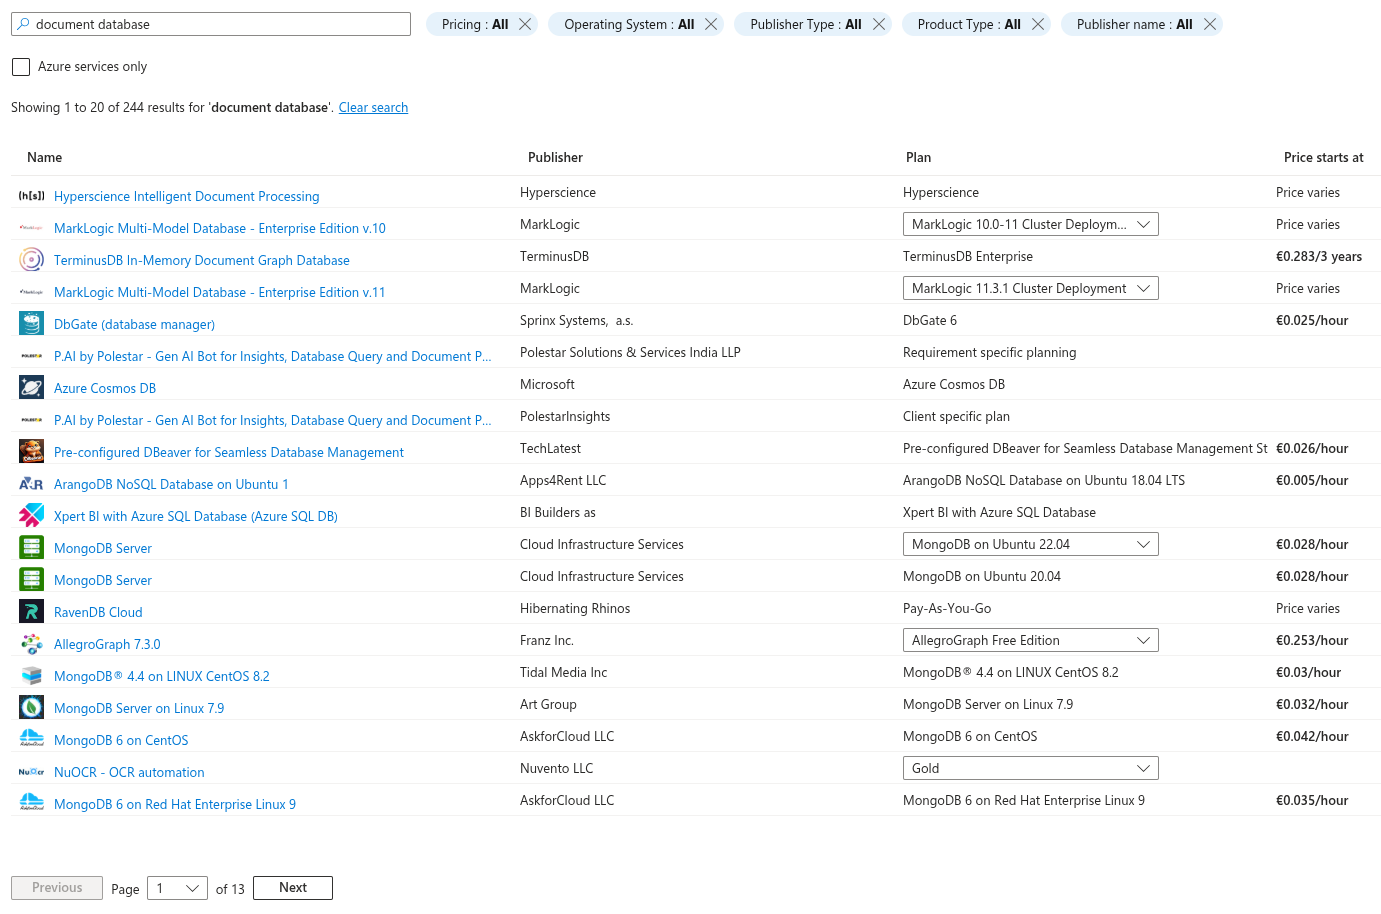
\includegraphics[width=\textwidth]{AzureDatabase.png}
    \caption{Proposte di Azure per i database documentali}
\end{figure}
\\
Azure Cosmos DB si distingue per la sua capacità di scalare orizzontalmente in maniera illimitata,
consentendo di gestire volumi di dati e carichi di lavoro molto elevati,
fino a milioni di richieste al secondo,
grazie alla possibilità di distribuire il carico su più regioni Azure.
È stato infatti ideato per presentare un'architettura distribuita,
con replica automatica dei dati,
assicurando un'elevatissima disponibilità e resilienza.
Queste vengono assicurate anche in caso di interruzioni regionali,
grazie a meccanismi di failover automatico.
Inoltre, la distribuzione globale garantisce che i dati siano sempre vicini agli utenti,
riducendo drasticamente la latenza a millisecondi
(con SLA del 99.999\% di disponibilità per account multi-regione).
Consente l'indicizzazione attraverso più partizioni in maniera
automatica e personalizzabile ottimizzando le query,
riducendo la complessità e migliorando le prestazioni,
senza richiedere oneri di gestione manuale degli indici.\\
\\
\begin{wrapfigure}{r}{0.25\textwidth}
    \centering
    
\includegraphics[height=.12\textheight]{cosmos.png}
    Azure Cosmos
\end{wrapfigure}
Pur essendo focalizzato sui database documentali,
Cosmos DB è però una soluzione multi-modello e multi-API.
Supporta infatti, oltre alla sua API nativa per NoSQL (che usa il modello a documenti JSON),
anche API compatibili con MongoDB, Apache Cassandra, Apache Gremlin (per i grafi) e Azure Table.
Questa versatilità permette agli sviluppatori di utilizzare strumenti familiari,
semplificando la migrazione di applicazioni esistenti o
lo sviluppo di nuove con la flessibilità di scegliere il modello di dati più appropriato.\\
\\
A livello di costi è difficile portare un'analisi precisa,
in quanto tutti i competitor presentano servizi
con capacità, disponibilità e intregrazione differenti.
I modelli di pagamento che utilizzano metriche di utilizzo diverse,
rendendo necessarie ulteriori analisi che dipendono anche
dall'effettiva tipologia e quantità delle richieste che vertono sul database.
Di seguito viene riportata una tabella per comparazione i costi delle alternative principali.
Cosmos usa come metrica le Rerquest Units(RU) per quantificare l'impatto di una richiesta sul database.
Le RU rappresentano un'astrazione delle risorse di sistema (CPU, I/O, memoria).
Ogni operazione consuma RU, proporzionalmente alla sua
complessità, dimensione e al carico computazionale richiesto.\\

\begin{longtable}{|P{3.2cm}|P{4.2cm}|P{4.2cm}|P{3cm}|}
    \hline
    \textbf{Servizio}      & \textbf{Costo ogni milione di scritture}\newline(normalizzate a 1 KB) & \textbf{Costo ogni milione di scritture}\newline (normalizzate a 1 KB) & \textbf{Costo di manutenzione GB/mese} \\
    \hline
    \endhead
    AWS DynamoDB           & \$1.25                                                                & \$0.25                                                                 & \$0.25                                 \\
    \hline
    Google Cloud Firestore & \$0.90                                                                & \$0.30                                                                 & \$0.156                                \\
    \hline
    Azure Cosmos DB        & In base al consumo di RU, \$5.84 al mese ogni 100RU/s                 & In base al consumo di RU, \$5.84 al mese ogni 100RU/s                  & \$0.25 (Transazionale)                 \\
    \hline
    \caption{Costi dei principali database documentali gestiti in Cloud}
\end{longtable}

La difficoltà di stabilirne il costo in una fase iniziale
è mitigata però dalla presenza di un piano gratuito perenne.
Cosmos DB offre infatti una quota gratuita di risorse iniziali,
per tutta la durata dell'utilizzo.
Il piano prevede 25 GigaByte di memoria gratuita,
a cui si aggiungono 1000 RU/s offerti per ogni categoria di operazione,
suddivise in lettura, scrittura ed eliminazione.
Dato lo stadio iniziale del progetto queste caratteristiche sono state considerate sufficienti,
permettendo di sfruttare e testare le capacità di distribuzione.
Nel caso in cui, sfruttando dati derivati dall'utilizzo effettivo dell'applicazione,
un'analisi condotta durante fasi successive del progetto faccia emergere che
Cosmos DB non rappresenti l’opzione più adeguata,
lo spostamento dei dati verso un altro gestore comporterà uno sforzo limitato,
data la compatibilità nella rappresentazione dei dati tra le diverse tecnologie di database documentali.

\subsection{La configurazione di Cosmos DB}

La creazione di una nuova istanza di Cosmos DB
richiede la definizione delle impostazioni di funzionamento,
che ne determinano le proprietà, a livello di disponibilità, ridondanza, sicurezza e resilienza ai guasti.\\
\\
La prima impostazione riguarda la distribuzione geografica dei dati.
Cosmos distribuisce sue risorse in zone, che vengono raggruppate in regioni.
L'opzione di usare delle availability zones duplica i dati su più zone all'interno della stessa regione.
Questo crea ridondanza dei dati per una maggiore resistenza ai guasti,
e così facendo aumenta la disponibilità dei dati,
che da un disponibilità garantita iniziale per la zona singola del 99.99\% (sulle scritture) sale al 99.995\%,
evitando la perdita dei dati e delle funzionalità in caso una zona non sia più raggiungibile.
L'aggiunta di ulteriori regioni diminuirebbe il rischio indisponibilità a causa di guasti
(i dati verrebbero duplicati anche tra le varie regioni),
ma aumenterebbe la complessità e il costo dell'applicazione.
Per una fase iniziale si è optato per garantire una ridondanza a livello di zone,
selezionando quindi l'opzione delle availability zones,
rimanendo però all'interno di una regione singola.\\

\begin{figure}[h!]
    \centering
    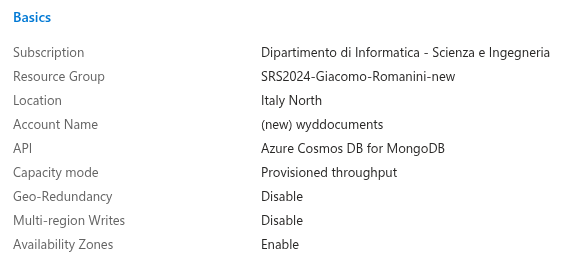
\includegraphics[width=\textwidth]{cosmosbasics.png}
    \caption{Impostazioni generali di Azure Cosmos DB}
\end{figure}

Volendo inizialmente rimanere in una singola regione,
l'impostazione "Geo-Redundancy" non è stata abilitata.
Allo stesso modo le scritture su più regioni non sono state abilitate,
preferendo un approccio centralizzato.\\
\\
Come modello di costo Azure propone due modalità distinte: Serverless e Provisioned throughput.
Nella modalità serverless il servizio scala in base alle richieste,
e considerando quindi solo l'effettivo utilizzo di risorse richieste.
Adatto a carichi di richieste improvvisi e sbilanciati,
non supporta l'esecuzione su più regioni.
Il provisioned throughput invece richiede una previsione delle risorse necessarie,
per metterle a disposizione e farsi pagare di conseguenza, che siano state usate o meno.
Questo necessita quindi di una stima del carico previsto,
per poi impostare le risorse.
Azure propone però un metodo chiamato autoscale,
che permette di modificare automaticamente (all'interno di un intervallo predefinito)
le risorse messe a disposizione in base al carico del momento,
per poi considerare il massimo valore raggiunto in quell'ora.
Questo permette di evitare l'implementazione di una strategia,
mantenendo comunque i costi legati al consumo effettivo delle risorse.
Prevedendo un carico di richieste non troppo elevato,
ma anche costante e poco variegato,
e considerando un tempo di latenza minore e il supporto a regioni multiple,
si è scelta una strategia di pagamento di tipologia provisioned throughput,
che verrà poi impostata per scalare automaticamente in un intervallo di risorse inizialmente contenuto.\\
\\
Per migliorare la sicurezza del database e garantire il controllo degli accessi
il database è stato inserito all'interno di una rete virtuale privata,
limitando l'accesso ai soli altri nodi che ne fanno parte,
isolandolo verso l'esterno.
Verranno quindi aggiunti alla rete solo i servizi che devono comunicare con Cosmos DB,
in particolare Azure Functions e il KeyVault(che contiene le chiavi per la cifratura dei dati).
Nonostante la ridondanza nelle zone garantisca il ritrovamento dei dati
anche in caso di indisponibilità di un'istanza del database,
si è scoperti qualora avvengano modifiche erronee o malintenzionate.\\
\\
Il servizio di backup proposto da Azure permette di salvare lo stato dei dati
fino a un certo momento nel passato,
in maniera tale garantire il ritorno a una situazione precedente
in caso ci si accorga siano avvenute modifiche non desiderate.
Azure permette sia di personalizzare la tipologia di backup,
in termini di durata, grandezza dei salvataggi e numero di copie,
sia di seguire delle opzioni già configurate.
Nel nostro caso si è scelto di applicare il servizio incluso gratuitamente
che mantiene le modifiche avvenute negli ultimi sette giorni.\\


\subsection{La definizione delle collezioni}

Stabilita la tipologia e il comportamento del servizio che ospita il database,
bisogna definire la struttura il cui le classi vengono salvate,
in maniera da sfruttare al meglio le sue proprietà,
allineando i dati alle procedure di lettura e scrittura,
per ottimizzare il carico e il tempo di risposta.\\
\\
Grazie alle proprietà di accoppiamento debole e al supporto alla denormalizzazione delle entità,
la libertà di modellazione del dominio fornita da Cosmos DB è massima.
Partendo dalle entità principali, per ognuna di esse è stata associata una collezione.
Sono state così definite quindi le entità di User, Profile, Event, Image e Group,
che rispondono agli omonimi elementi del dominio.
A Event e Profile si aggiungono ProfileDetails ed EventDetails,
che contengono i dati particolari di questi elementi.
Gli Account sono gestiti internamente da Firebase Authentication,
e la loro relazione con gli utenti è stata mappata in un insieme all'interno di User
tramite i loro Uid.\\
\begin{figure}[htbp]
    \centering
    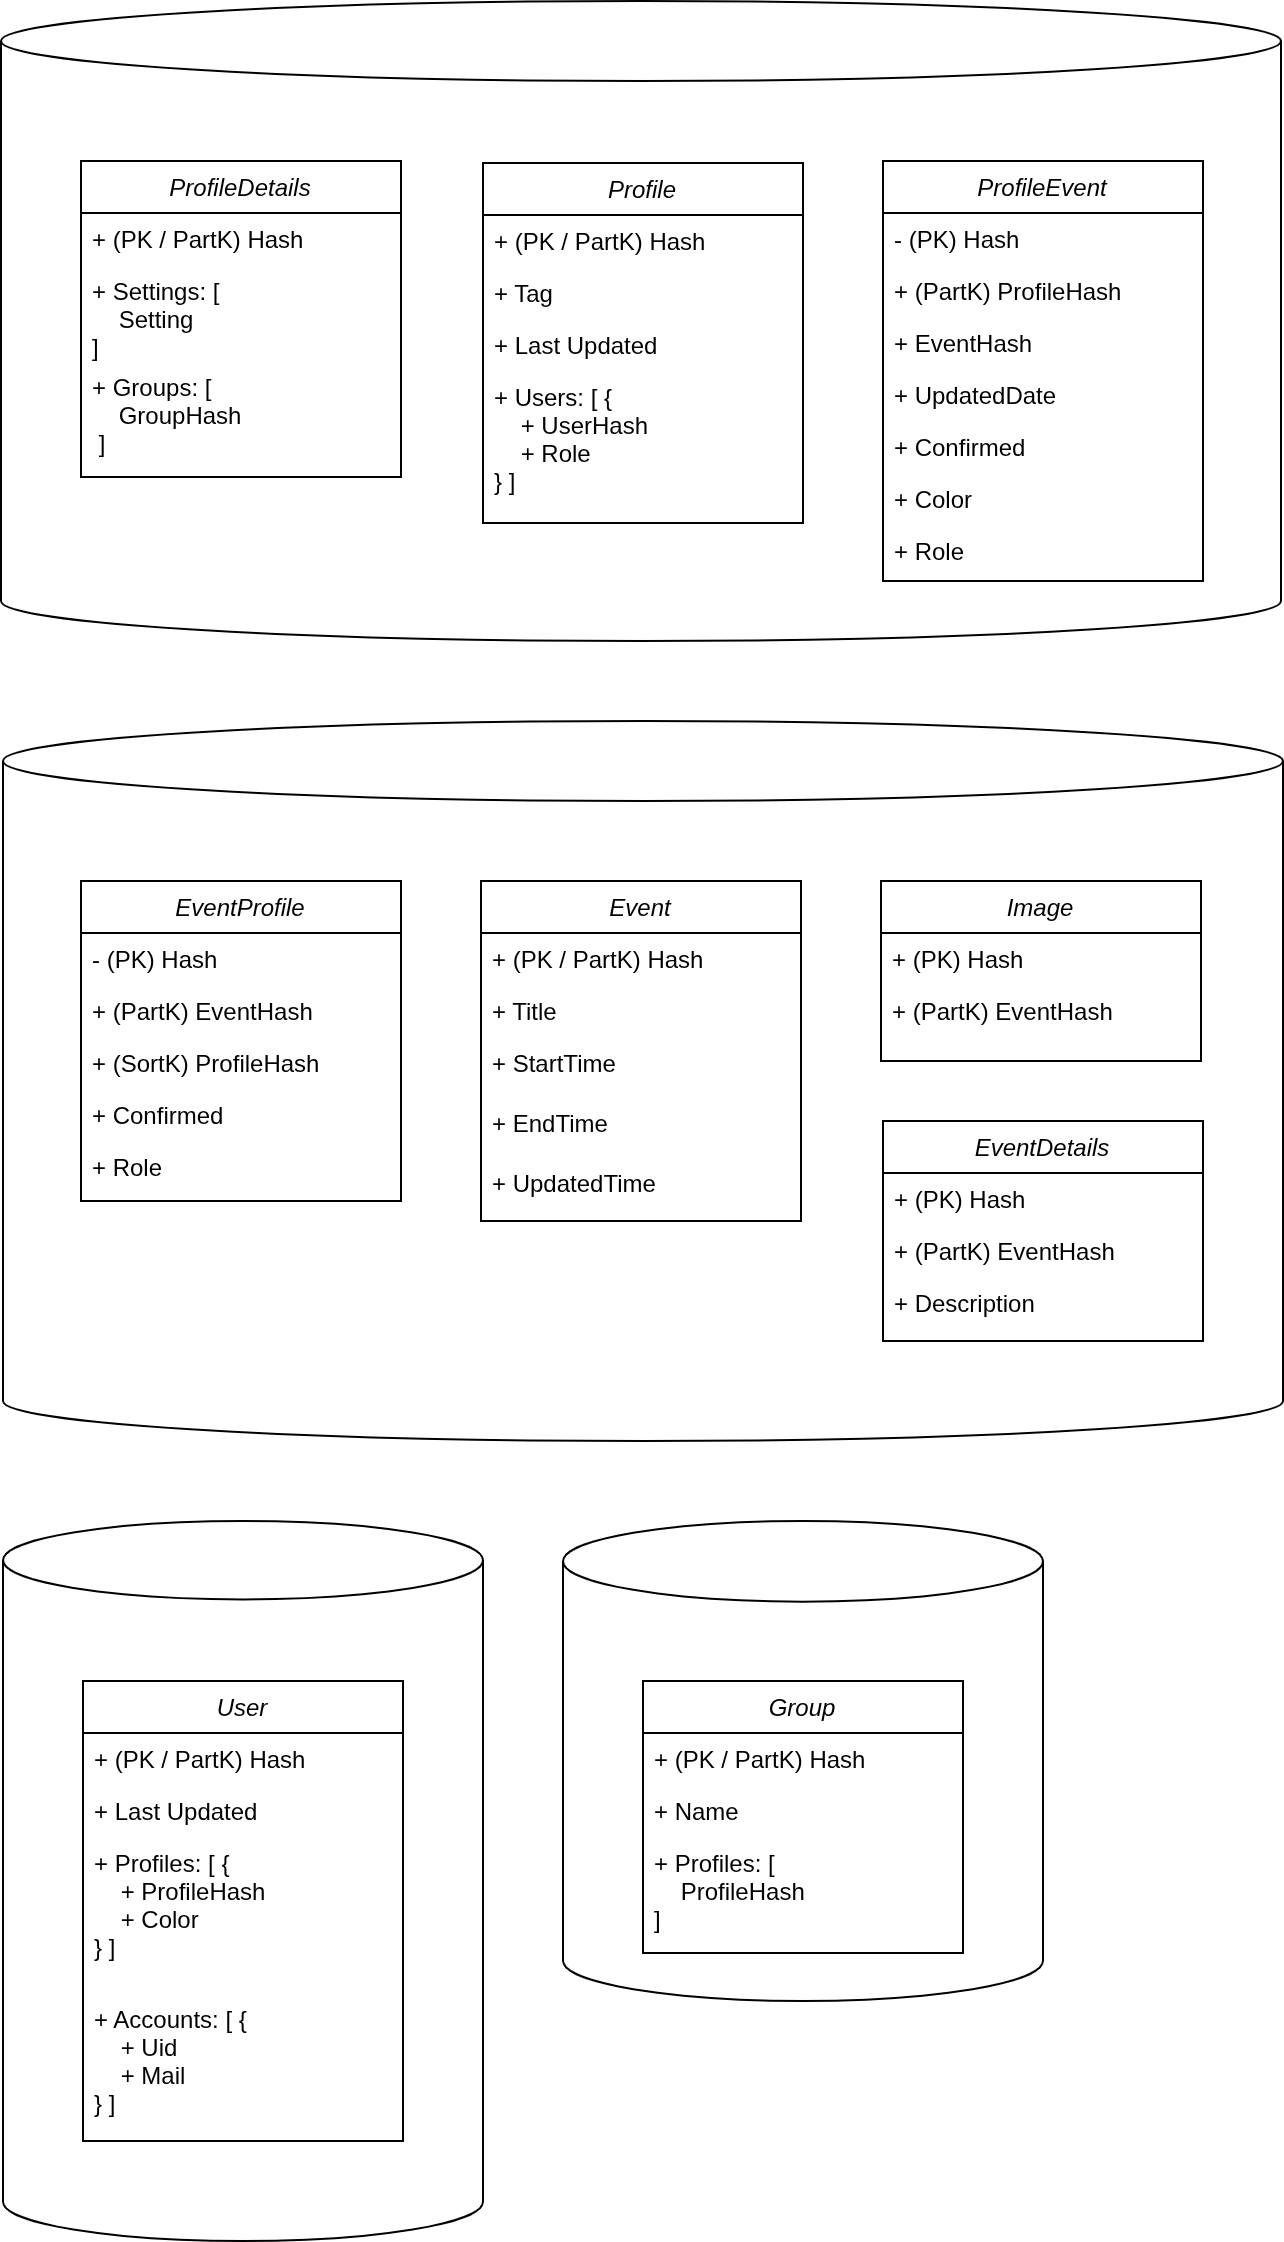
\includegraphics[height=.96\textheight]{NonRelazionalModel.png}
    \caption{Modello delle collezioni e il loro partizionamento}
\end{figure}
\\
Allo stesso modo, laddove siano presenti relazioni uno a molti con cardinalità contenute,
è stato possibile integrarle all'interno degli oggetti stessi, duplicando i collegamenti.
Si evita così la necessità di cercare e recuperare i dati, 
rendendoli già direttamente disponibili.
È il caso delle immagini, in cui viene salvato il riferimento dell'Event in Image,
o di User e Profile, i quali contengono entrambi i corrispettivi riferimenti.
UserRole è stato integrato solo in ProfileDetails,
essendo necessario per controllare i permessi di un utente verso un profilo, e non il contrario.\\
\\
La relazione tra profili e gruppi vede invece cardinalità elevate:
non è infatti posto un limite al numero di gruppi a cui un profilo può fare parte.
Non richiedendo però dettagli particolari o interazioni complicate (in questa fase del progetto),
è stato considerato sufficiente mappare le relazioni tramite liste all'interno di Group e ProfileDetails.\\
\\
Come analizzato nelle sezioni precedenti,
le richieste del progetto vertono sulla relazione tra eventi e profili.
In particolare, le richieste che sono previste più frequenti e quindi impattanti
sono quelle di recupero dei dati generali delle entità su entrambi i versi della relazione
(eventi relativi ai profili o profili collegati agli eventi),
ma anche di conferma di un evento.
Per prima cosa, vista la centralità delle richieste su queste entità,
sono state separate le proprietà di dettaglio da quelle essenziali,
salvandole in ProfileDetails ed EventDetails.\\
\\
Oltre a migliorare il tempo di recupero delle informazioni
che si ritiene necessario essere immediatamente disponibili, 
si evita così che le operazioni che vertono su dati secondari 
impattino sul flusso principale delle richieste.
Riducendo la mole di dati da recuperare e analizzare,
si rendono le query relazionali meno pesanti e più veloci.\\
\\
Prevedendo richieste di conferma sullo stesso evento molto vicine tra loro
si è deciso di non integrare la relazione nelle entità esistenti,
bensì di esternarla in documenti dedicati,
per evitare modifiche concorrenti sullo stesso Event.
Si introduce così ProfileEvent,
che presenta tutte le proprietà della relazione tra i due elementi.
Venendo partizionato in base all'hash del profilo corrispondente,
assolve il compito di recuperare gli eventi associati al profilo.
Include quindi il collegamento all'evento e
la conferma o meno della partecipazione del profilo all'evento,
ma anche la data dell'ultimo aggiornamento del profilo associato,
in maniera tale da consentire di controllare direttamente
se un evento è stato modificato rispetto all'ultimo aggiornamento,
e deve quindi essere caricato.\\
\\
Si prevede però che la quantità di richieste sia comunque importante
anche dal lato opposto della relazione,
ovvero per ottenere i profili correlati agli eventi.
Non è accettabile una ricerca che attraversi le partizioni per recuperare queste informazioni.
Per questo motivo viene creato EventProfile,
che, partizionato assieme agli eventi,
mantiene le informazioni minime necessarie per mostrare i profili collegati,
in maniera da limitare la quantità di dati da mantenere consistente.\\
\\
La distribuzione dei dati supporta così la scalabilità totale del sistema.
Ogni richiesta di dati infatti non incrocia mai più di due elementi,
e rimane in ogni caso limitata alla sua partizione.
Lo stesso può essere affermato per le richieste di modifica, 
le quali vertono su un unico elemento principale considerato come fonte di verità,
in base al quale le eventuali copie dovranno essere aggiornate.
Se è vero che le richieste sono state rese rapide 
sia in lettura che in scrittura,
questo è reso possibile grazie alla denormalizzazione, 
che deve però prevedere un procedimento per l'allineamento
dei dati copiati.\\

\subsection{L'integrazione con le Azure Functions nel framework .Net}
L'utilizzo di un database documentale comporta un sviluppi implementativi specifici.
Il polimorfismo dei documenti e la denormalizzazione delle entità
rendono la rappresentazione logica degli elementi e la loro relazione reciproca di secondaria importanza.
L'approccio a oggetti del Framework .Net assume quindi minore rilevanza,
in quanto si rende meno necessaria la capacità di descrivere e astrarre
le entità logiche attraverso classi di codice.
Si distinguono però due tipologie di richieste principali,
che determinano l'approccio apportato verso i dati:
la recupera di un elemento e la sua modifica.\\
\\
Quando è necessario recuperare un elemento dal database risulta comodo
convertirlo in un oggetto.
Questo consente di gestire le informazioni attraverso un'astrazione logica, con tutti i vantaggi relativi.
La sua utilità risalta sopratutto nel caso in cui la lettura dell'elemento
non ha il solo fine di essere restituito al richiedente,
ma deve venire analizzato per procedere con la logica applicativa.
La rappresentazione dei documenti in oggetti comporta infatti un codice più pulito e ordinato,
interagendo con le proprietà e i metodi della classe, senza entrare nella complessità computazionale
dell'elaborazione del documento.
La conversione viene svolta automaticamente dal framework,
e permette di associare ai dati il codice strettamente relativo, creando metodi appositi.\\
\\
Ogni elemento del dominio avrà quindi una classe associata,
con tutti i campi previsti dal modello.
Il contesto logico così introdotto agevola l'interazione tra i servizi e gli oggetti,
riducendo la probabilità di errori e semplificandone l'individuazione.
Anche il testing viene favorito, dando la possibilità di analizzare il codice
senza la necessità di interrogare il database o di simularlo.
Permette inoltre di automatizzare la conversione dei dati verso i DataTransferObject(DTO),
necessari per uniformare le risposte verso i client,
che contribuiscono a separare la logica di business da quella che gestisce la comunicazione.\\
\\
Nel caso la richiesta richieda invece la modifica di un elemento
la conversione del documento in oggetto risulta poco efficiente.
La creazione di un nuovo oggetto comporta infatti l'intera lettura dell'elemento associato.
Questo può essere utile se è necessario mantenere un riferimento logico,
se si useranno le informazioni che contiene
o se bisognerà restituire al mittente l'oggetto aggiornato.
Nella maggior parte dei casi invece si vuole semplicemente applicare una modifica,
lasciando che sia il sistema a propagarla.
In tal caso, Cosmos DB permette le cosiddette patch update,
ovvero modifiche limitate al campo interessato,
senza richiedere la lettura e la sovrascrittura dell'intero documento.
Per queste occasioni vengono implementati appositi metodi che,
preso in ingresso i dati da modificare,
interagiscono con il database per aggiornare le sole parti coinvolte.\\
\\
La comunicazione con il database viene astratta tramite un servizio dedicato chiamato WydDbService.
WydDbService ha il compito di gestire le richieste e le sessioni con il database,
nascondendo le complessità implementative e di interazione.
In particolare, la connessione con il database comporta
la richiesta verso Azure Key Vault per il recupero delle chiavi di accesso,
per poi usarle per stabilire un canale attraverso il quale applicare le modifiche.
Mette inoltre a disposizione un'interfaccia per nascondere
tutte le logiche di basso livello dovute dall'interazione specifica di CosmosDB.
Verrà utilizzato dagli altri servizi tramite dependency injection,
automatizzandone la creazione e l'utilizzo, e di conseguenza la connessione e le richieste al database. \\

\subsection{Garantire la consistenza eventuale dei dati}

Avendo salvato le entità del dominio sotto forma di documenti denormalizzati
la modifica del campo di un elemento potrebbe dover comportare la necessità
di propagare gli aggiornamenti su tutti gli altri componenti in cui tale dato è duplicato.\\
\\
Potendo accettare un ritardo nell'allineamento dei dati,
è possibile separare la modifica del documento principale
dalla sua distribuzione sul resto del database.
Affidare il compito di aggiornare tutti i componenti secondari coinvolti
alla stessa funzione risulta svantaggioso sotto molti aspetti.
Si introdurrebbe infatti un ritardo nell'esecuzione,
dovuto all'attesa dell'applicazione delle ulteriori modifiche,
che devono essere controllate e gestite in caso falliscano.
Complicare la funzione va inoltre contro i principi stessi
dei servizi serverless,
che prevedono invece strutture semplici con responsabilità precise e limitate.
La loro efficienza deriva infatti dalla possibilità
di eseguire in maniera autonoma compiti specifici.
L'unico requisito necessario per permettere a una funzione di delegare ad altre le modifiche derivate
è la garanzia che la loro esecuzione venga controllata e che quindi il loro successo sia assicurato.\\
\\
L'introduzione di una funzione con il ruolo di orchestratore
non sposterebbe di molto il problema.
Nonostante soddisfi la necessità di affidare a diverse funzioni
le diverse parti del problema e sia in grado di controllarne il risultato,
potendone così garantire il successo,
implica comunque l'attesa del loro completamento.
Aggiungerebbe inoltre un ritardo dovuto al tempo necessario per la sua stessa esecuzione,
che aspetta e controlla le funzioni che ha chiamato.
Questo ritardo è negativamente influenzato dall'accoppiamento debole
tra l'orchestratore e le funzioni figlie,
che non assicura l'immediata ripresa del padre 
al termine dell'esecuzione di una funzione da lui chiamata.
Le dipendenze che verrebbero così introdotte tra 
l'orchestratore, la funzione originale e quelle necessarie per la consistenza dei dati,
comporterebbero solo rischi di fallimento e l'allungamento dei tempi di risposta.\\
\\
A questo scopo, Azure Cosmos DB mette a disposizione uno strumento apposito, chiamato Change Feed.
Change Feed è un meccanismo tramite il quale è possibile
associare le modifiche di un elemento del database
all'esecuzione di una funzione.
Il Change Feed viene definito come trigger all'interno di una funzione,
e viene associato a una collezione di documenti.
Ogni volta che un documento di questa collezione subisce un aggiornamento
si crea in automatico un log che,
all'interno della partizione coinvolta,
viene salvato in una nuova collezione dedicata chiamata "lease".
Il Change Feed è dunque il meccanismo che,
nel momento in cui un log viene aggiunto alla sua lease,
fa partire autonomamente la funzione associata.\\
\\
Una volta invocata,
la funzione legge dal lease tutti i log che non sono ancora stati processati
per poi propagare le modifiche ove necessario.
L'avvenuto successo dell'elaborazione del log viene registrato
grazie a dei token di aggiornamento,
che permettono di sapere in quale punto del lease 
sono presenti i log che non sono ancora stati processati.
La persistenza dei log sui lease garantisce
che la modifica sia presa in carico da una funzione almeno una volta,
mentre la presenza dei token di aggiornamento assicura
che la funzione venga eseguita di nuovo in seguito a un errore o a un guasto del sistema,
soddisfando così i requisiti di invocazione.
Questo meccanismo è intrinsecamente scalabile.
Essendo infatti i lease associati alle partizioni in cui risiedono i documenti,
è possibile dividere (e quindi distribuire, quando necessario) il carico su più funzioni.\\
\\
Il Change Feed viene usato, ad esempio,
nel caso in cui venga cambiata un'informazione importante di un evento.
Questa operazione comporta l'aggiornamento di UpdatedDate,
campo che memorizza il momento in cui è stata apportata l'ultima modifica.
UpdatedDate è stata denormalizzata all'interno dei ProfileEvent,
e la sua modifica deve essere quindi propagata.
La propagazione di questo aggiornamento sarà delegata a una seconda funzione.
L'invocazione di questa funzione verrà associata
al lease relativo alla collezione degli Event,
nel caso siano presenti log non ancora elaborati.
In questa maniera i compiti vengono efficacemente suddivisi in due funzioni,
indipendenti tra loro.
La prima funzione avrà il solo compito di cambiare la proprietà dell'oggetto,
informando il client riguardo al successo dell'operazione.
Una seconda funzione, attivata in autonomia dal Change Feed,
si occuperà poi di aggiornare tutti i ProfileDetails relativi,
senza andare a impattare sulle prestazioni o sulle dipendenze della prima.\\
\\
Ci sono situazioni in cui il Change Feed non può essere usato.
È ad esempio il caso della conferma di un evento.
L'elemento primario coinvolto in questa operazione è ProfileEvent,
che sarà modificato dalla funzione iniziale.
La conferma di partecipazione a un evento da parte di un profilo
viene considerato come modifica all'evento stesso,
che comporta quindi l'aggiornamento del documento Event.
Se però si associasse una funzione anche per le modifiche a ProfileEvent tramite Change Feed,
si verrebbe a creare una ricorsione infinita per il quale 
la modifica a un ProfileEvent comporta la modifica a un Event, 
che a sua volta comporta una modifica a ProfileEvent, e via dicendo.
Per quanto sia possibile aggiungere all'interno delle funzioni controlli
che analizzino ogni volta l'origine della richiesta,
questo porterebbe a una maggiore complessità e a un aumento del carico implementativo,
introducendo nuovi dati all'interno di ogni aggiornamento.
Si è quindi deciso di utilizzare il ChangeFeed solo per le entità
la cui modifica influenza molteplici altri documenti,
delegando in maniera differente l'eventuale aggiornamento di un altro elemento singolo.\\
\begin{figure}[htbp]
    \centering
    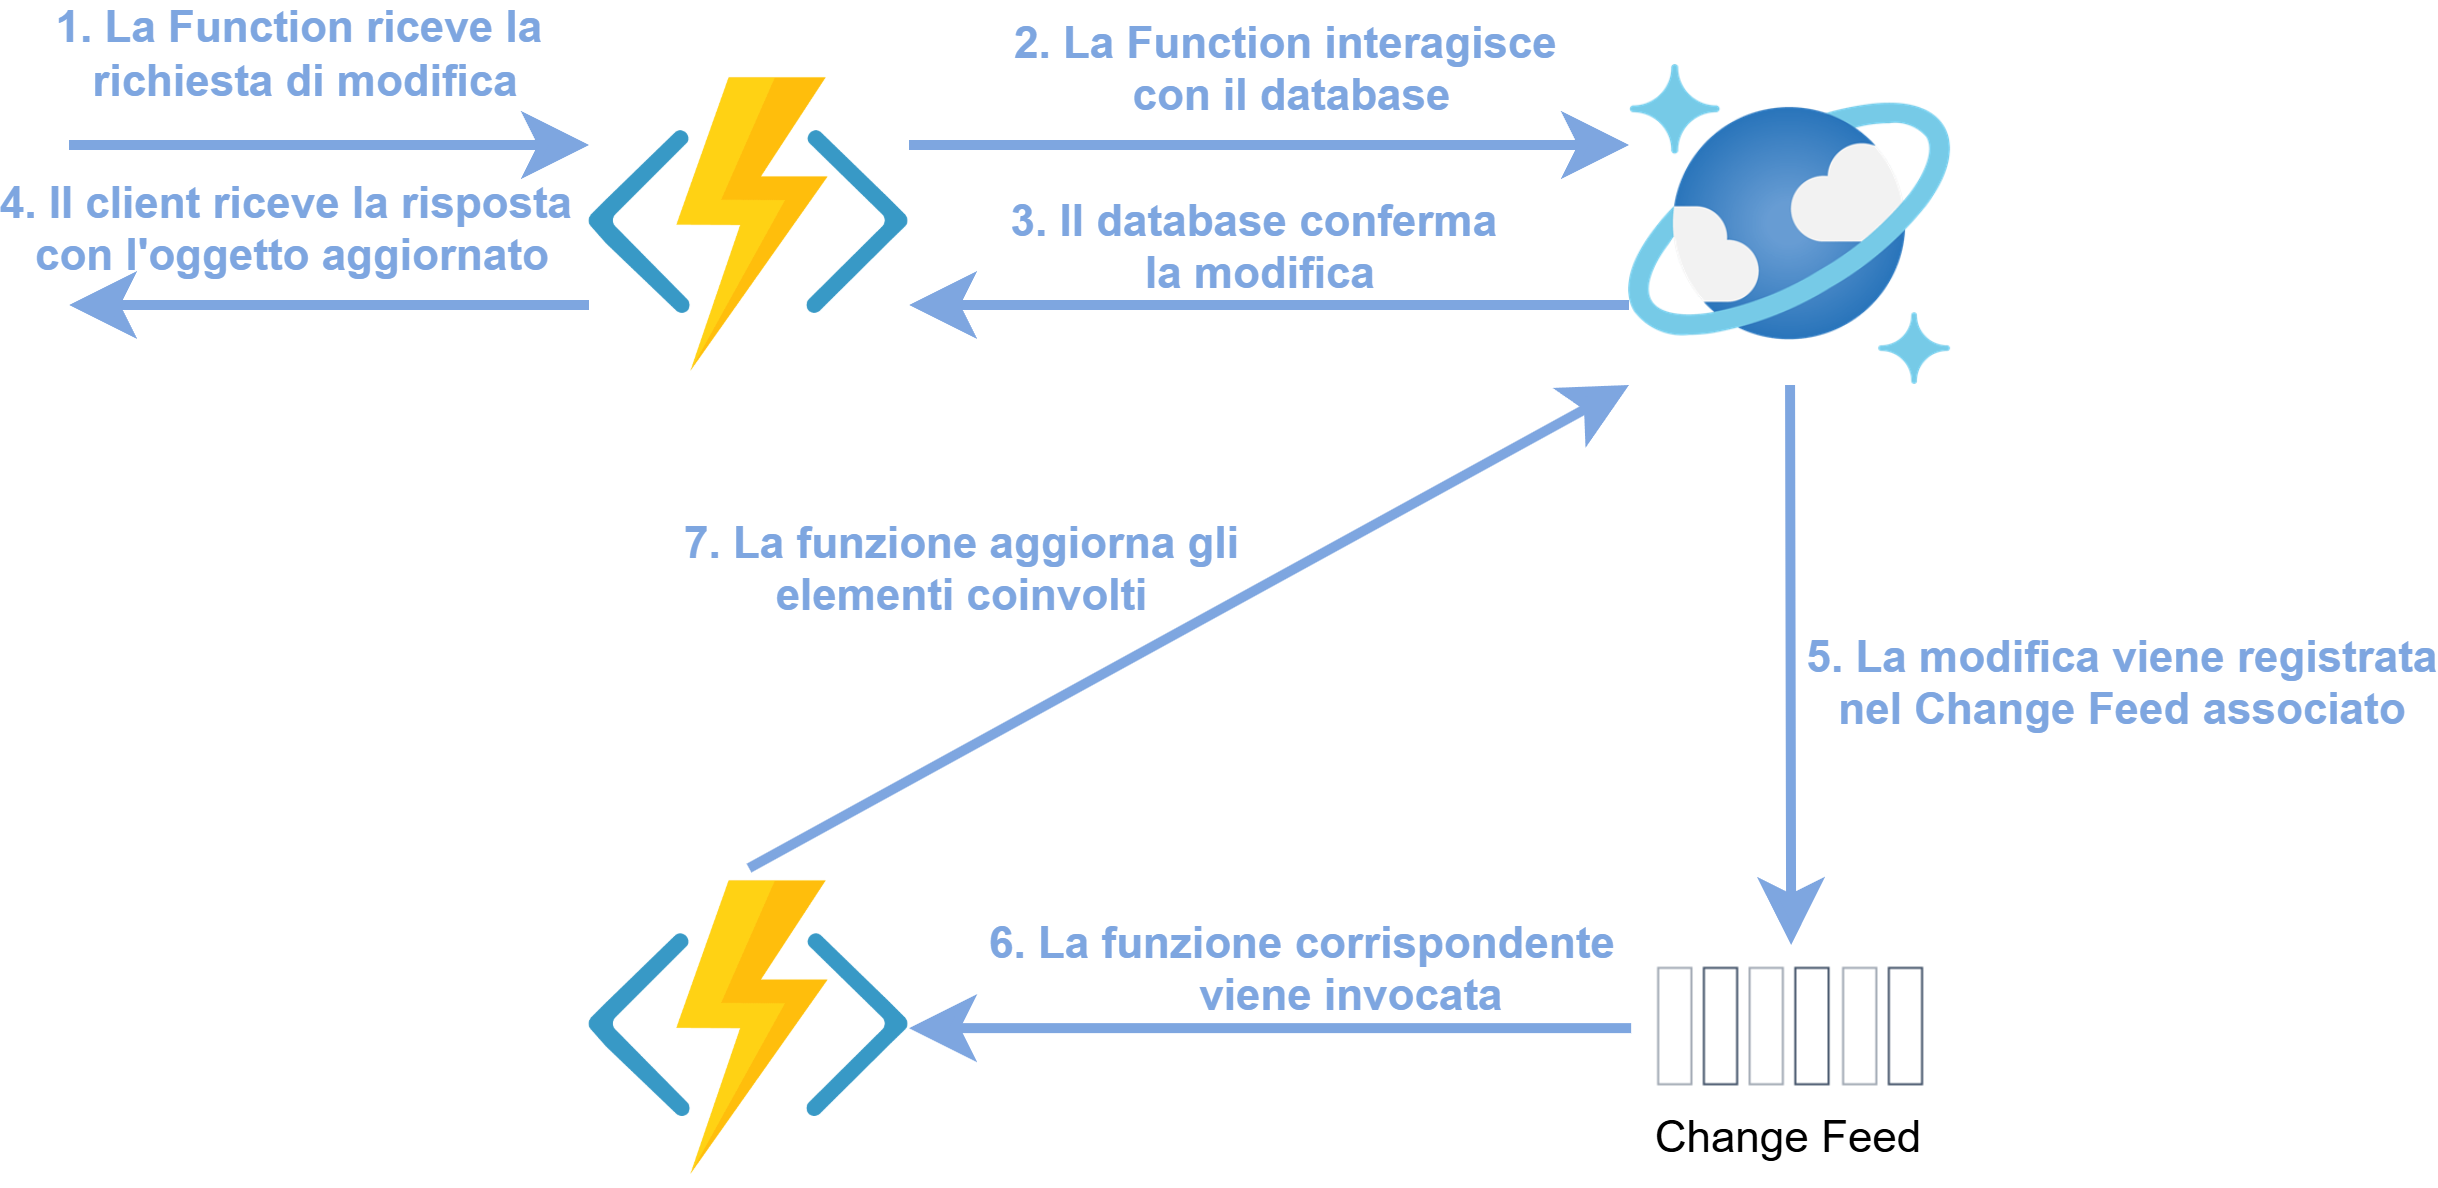
\includegraphics[width=\textwidth]{EventChangeFeed.png}
    \caption{Aggiornamento dei documenti tramite Change Feed}
\end{figure}\\
Ci sono diversi modi che le Azure Functions possono sfruttare
per invocare un'altra funzione, senza passare per l'utilizzo di un orchestratore.\\
\\
Una prima soluzione può essere l'invio di una nuova richiesta HTTP al server stesso,
al quale è associata la funzione voluta.
Per quanto risulti veloce e facile da implementare,
questa soluzione non garantisce l'effettiva presa in carico, esecuzione e completamento della richiesta,
a meno di controllarne la risposta.
Il controllo della risposta comporta però l'attesa della richiesta,
procedimento che mina la finalità stessa dell'operazione.\\
\\
Azure mette invece a disposizione servizi basati su code ed eventi
proprio per mettere in comunicazione diverse parti di uno stesso sistema.
Tra le funzionalità offerte da Azure e
quindi direttamente integrabili con le Azure Functions troviamo
Azure Queue Storage, Azure Service Bus e Azure Event Hub.\\
\\
Azure Queue Storage è un servizio di code di messaggi
offerto come parte di Azure Storage,
che si occupa del salvataggio di informazioni
che non rientrano nei casi d'uso dei database tradizionali.
Le funzioni hanno quindi la possibilità di aggiungere alla coda i propri messaggi,
che verranno poi elaborati da un'altra funzione grazie a un trigger associato.
La dimensione massima che i messaggi possono avere è di 64 KB,
e rimangono in memoria per un tempo prestabilito, che può essere configurato.
Le code sono persistenti e altamente disponibili,
assicurando che i messaggi non vadano persi in caso di fallimento del consumer,
ma non presentano ulteriori funzionalità associate.\\
\\
La sua semantica di consegna garantisce che il messaggio venga elaborato almeno una volta,
il che significa che la sua consegna potrebbe avvenire più volte,
in caso di errori o di timeout di elaborazione da parte della prima funzione che lo ha preso in carico.
Presenta quindi un servizio semplice e veloce,
estremamente robusto ma anche scalabile.
La sua semplicità, sebbene contribuisca a ridurne il costo,
ne comporta però la mancanza di ulteriori proprietà avanzate.
Ad esempio, Azure Queue Storage non presenta la capacità
di gestire i messaggi in caso la loro esecuzione continui a fallire,
che può essere desiderata in caso sia necessario assicurare che l'operazione giunga al suo termine.\\
\\
Azure Service Bus è invece un servizio di messaggistica
che supporta scenari più complessi rispetto a Queue Storage.
Offre due tipologie principali di comunicazione: code e argomenti.
Le code di Service Bus supportano le stesse funzionalità del servizio precedente,
a cui però se ne aggiungono di più avanzate quali l'ordinamento,
le sessioni per il raggruppamento di messaggi correlati,
la funzionalità di "dead-letter queue" integrata per la gestione automatica dei messaggi non elaborabili e
l'elaborazione transazionale.\\
\\
Gli argomenti(topic) prevedono un pattern publish/subscribe,
nel quale più fruitori possono collegarsi allo stesso argomento per poi
venire tutti notificati in contemporanea in caso venga inviato un messaggio a esso inerente.
Essendo stato progettato per soddisfare carichi di lavoro aziendale,
oltre a fornire garanzie di consegna più robuste e
integrare meccanismi di gestione degli errori,
garantisce un'elevata scalabilità.
Risulta però più costoso e relativamente più complesso da utilizzare.\\
\\
Azure Event Hub è un servizio di ingestione di dati altamente scalabile e a bassa latenza,
progettato per lo streaming di grandi volumi di eventi da diverse fonti.
Non è una coda di messaggi nel senso tradizionale,
ma piuttosto un "broker di eventi",
in cui gli eventi vengono aggiunti a una coda distribuita su più partizioni
dove rimangono disponibili per i consumer per un periodo configurabile (fino a 90 giorni).
I consumer leggono gli eventi dalla partizione mantenendo ognuno il proprio progresso,
il che permette a più consumer group di leggere gli stessi eventi indipendentemente.\
Anche in questo caso, la semantica garantisce che il messaggio venga elaborato almeno una volta.\\
\\
Presenta quindi elevate caratteristiche di scalabilità,
fornendo una bassa latenza, un throughput estremamente elevato
e la possibilità di parallelizzare il consumo dei messaggi.
Pur mantenendo in memoria i dati,
e quindi assicurando che sia sempre possibile applicare le modifiche,
tutta la logica necessaria per controllare l'esecuzione, ritentare ed eliminare il messaggio
rimane però a carico dello sviluppatore.\\
\begin{longtable}{|P{2.9cm}|P{3.9cm}|P{3.9cm}|P{3.9cm}|}
    \hline
    \textbf{Caratteristica} & \textbf{Queue Storage}                                         & \textbf{Service Bus}                                                              & \textbf{Event Hub}                                                      \\
    \hline
    Tipo di servizio        & Coda di messaggi semplice                                      & Coda/Broker di messaggi                                                           & Flusso di eventi                                                        \\
    \hline
    Modalità di fruizione   & Competing Customers (Point-to-point)                           & Competing Customers (Point-to-point)\newline Publish/Subscribe (argomenti)        & Publish/ Subscribe (molti a molti)                                      \\
    \hline
    Caratteristiche         & Semplice, scalabile e robusto ma nessun controllo degli errori & Affidabile, scalabile, garantisce il controllo dell'esecuzione, ordina i messaggi & Scalabile, robusto, ordinato ma nessun controllo sull'esecuzione        \\
    \hline
    Costo                   & €0,04 GB/mese + €0.0004 ogni diecimila operazioni              & €0,044 ogni milione di operazioni (piano Basic con solo le code)                  & €0,014/ora per ogni Unità di throughput + €0,025 ogni milione di eventi \\
    \hline
    \caption{Proprietà dei servizi Azure per la propagazione interna di messaggi }
\end{longtable}

\begin{wrapfigure}{r}{0.25\textwidth}
    \centering
    
\includegraphics[height=.12\textheight]{servicebus.png}
    Service Bus
\end{wrapfigure}
Viste queste considerazioni,
per garantire la consistenza degli oggetti nei casi in cui non sia possibile sfruttare il Change Feed
si è scelto di adottare Azure Service Bus.
La scelta deriva principalmente dalla suo supporto nativo al controllo dell'esecuzione delle funzioni,
grazie all'utilizzo di una dead-letter queue.
La dead-letter queue è un contenitore in cui vengono inseriti
tutti i messaggi la cui elaborazione è stata tentata e fallita una determinata quantità di volte.
Garantisce quindi, in aggiunta a ulteriori tentativi in caso di insuccesso,
il monitoraggio di tutte le operazioni che non riescono a essere portate a termine.
Questo permette di assicurare che gli aggiornamenti necessari per allineare i documenti
siano sempre controllati.\\
\\
Tornando all'esempio precedente,
nel quale era necessario propagare la conferma di un evento,
la modifica di Event e di EventProfile verrà eseguita da due funzioni dedicate.
Al termine della modifica di ProfileEvent,
la funzione inserirà in coda al Service Bus un messaggio
con le informazioni necessarie alle altre due,
per poi inviare la risposta al client.
Le due funzioni verranno quindi invocate,
aggiornando gli elementi coinvolti.
Nel caso di Event, il Change Feed associato aggiornerà di conseguenza
tutti i sui ProfileEvent, senza però creare ricorsioni.\\

\begin{figure}[h!]
    \centering
    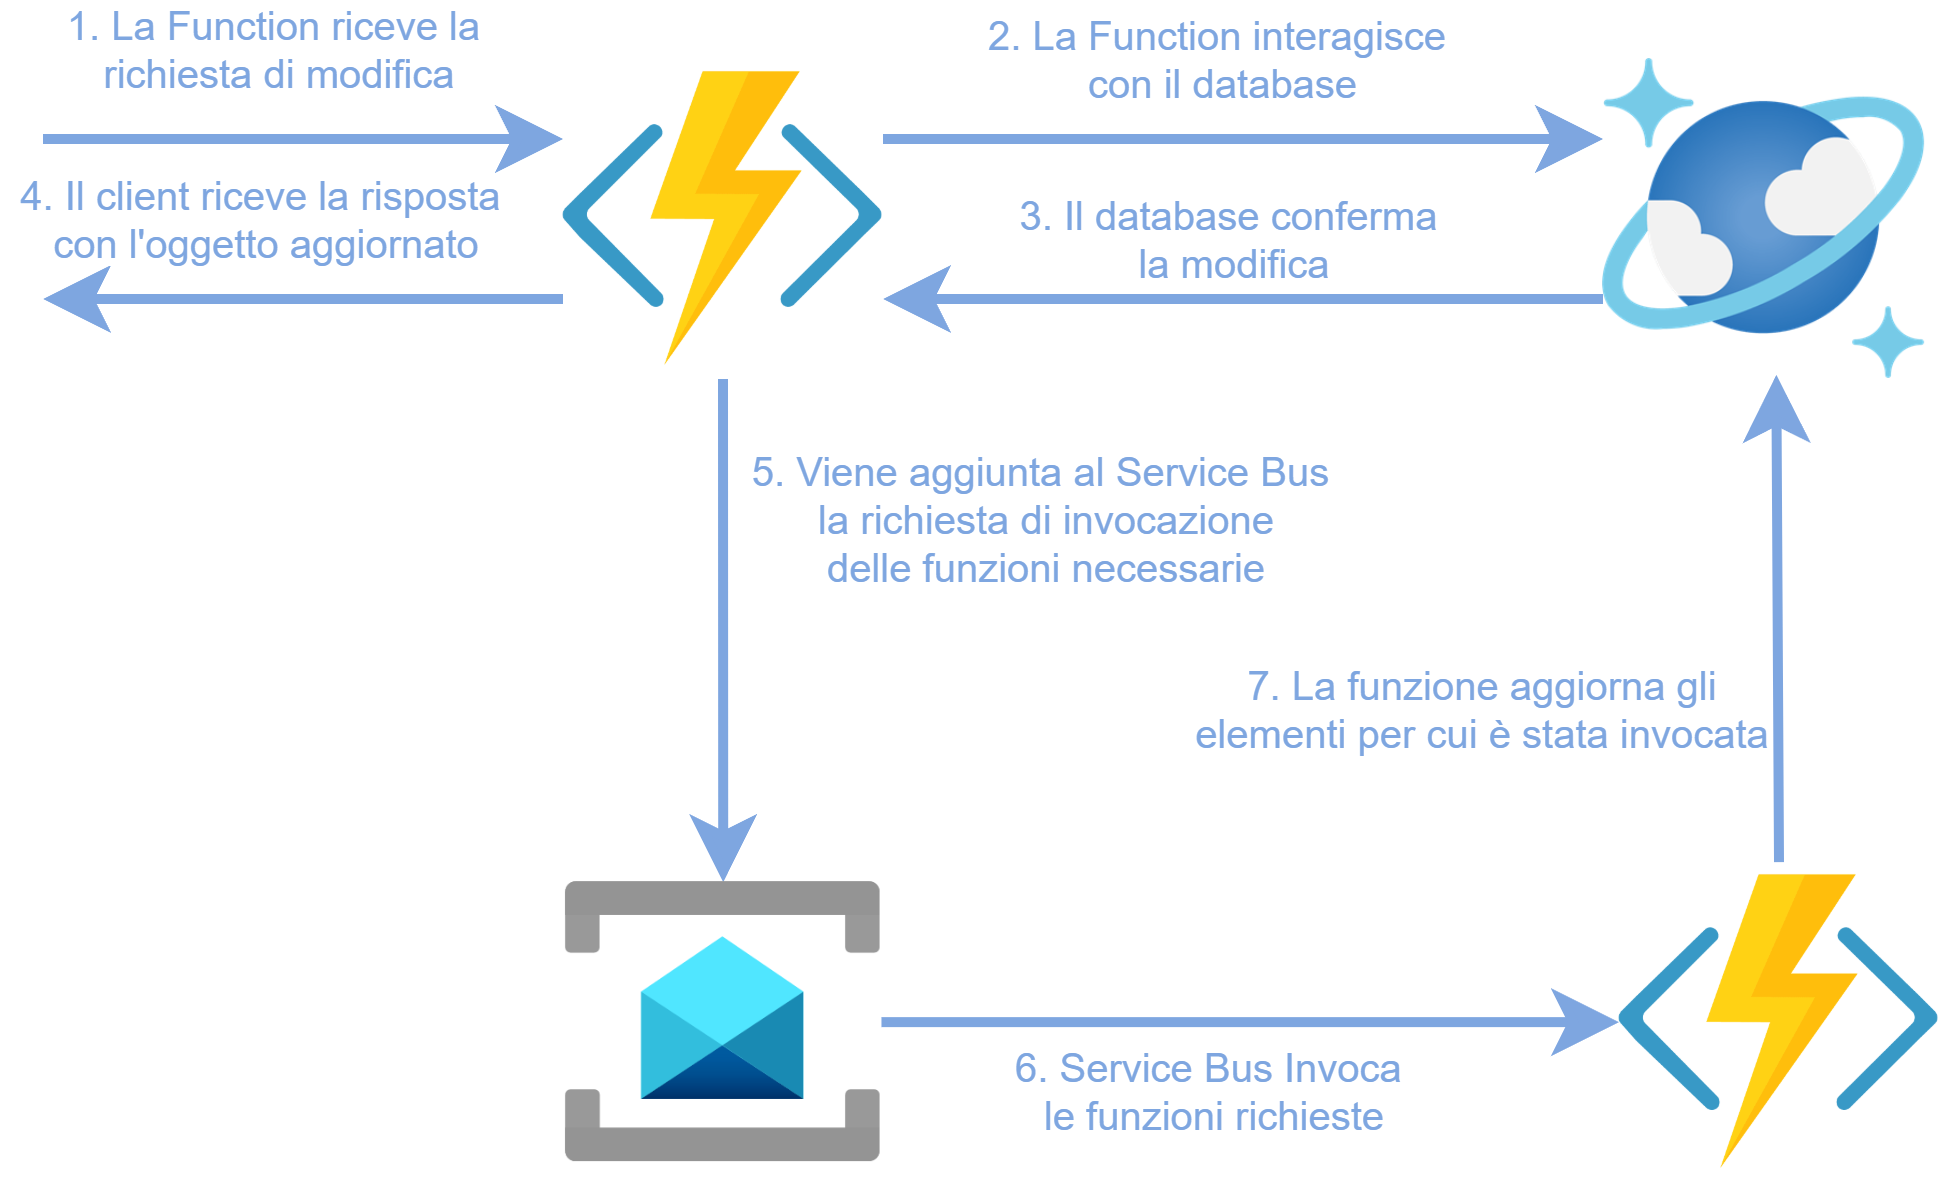
\includegraphics[height=0.39\textheight]{EventServiceBus.png}
    \caption{Fasi di aggiornamento tramite Service Bus}
\end{figure}




\clearpage
%\chapter{Il recupero ed il salvataggio dei dati multimediali}

I file multimediali rappresentano un elemento centrale all’interno di un’applicazione orientata alla condivisione sociale,
contribuendo significativamente all’esperienza utente e all’interazione tra i partecipanti.
La possibilità di acquisire e condividere contenuti visivi, come immagini e video, consente di documentare eventi e attività,
favorendo una memoria collettiva e rafforzando il legame tra gli utenti.
In particolare, l’integrazione di materiale multimediale associato a eventi condivisi permette di preservare una rappresentazione più completa e dettagliata dell’esperienza vissuta,
migliorando l’engagement e la partecipazione all’interno della piattaforma, rappresentando uno dei punti di forza dell’applicazione.\\
\\
Tuttavia, la gestione dei file multimediali introduce complessità operative sia per gli utenti sia per il sistema stesso.
Da un lato, la selezione e l’invio dei contenuti possono rappresentare un onere significativo per l’utente, aumentando l’attrito nell’utilizzo dell’applicazione.
Per ottimizzare il processo e migliorare l’usabilità, è essenziale semplificare al massimo l’interazione richiesta,
automatizzando il recupero dei dati e limitando il ruolo dell’utente alla semplice conferma dei contenuti selezionati.
Questo approccio non solo semplifica l’esperienza d’uso, ma la rende più intuitiva e fruibile,
contribuendo anche a un incremento del tasso di adozione e della frequenza di utilizzo dell’applicazione.\\
\\
Parallelamente, la memorizzazione e il trasferimento di file multimediali pongono sfide significative a livello infrastrutturale,
in quanto tali dati presentano un impatto rilevante sulle risorse computazionali e sulla gestione dello storage.
Il volume elevato di richieste di caricamento e accesso ai file può infatti compromettere le prestazioni del sistema,
introducendo ritardi causati dal traffico di azioni che potrebbero influire negativamente sulle altre operazioni dell’applicazione.
Per garantire un’archiviazione efficiente e scalabile, è quindi necessario implementare una strategia di gestione della memoria
che separi il salvataggio dei file multimediali dal database principale, evitando di sovraccaricare il server applicativo.
Questa soluzione deve inoltre garantire un aggiornamento tempestivo delle informazioni, assicurando la sincronizzazione tra i dati archiviati e le modifiche effettuate dagli utenti.\\
\\
Per affrontare tali problematiche, un primo esame osserverà le modalità di recupero dei file multimediali,
con un focus sulle tecniche di selezione e rilevamento automatico delle immagini, nonché sui vincoli normativi e di sicurezza che ne regolano l’utilizzo.
In un secondo tempo l’analisi si concentrerà invece sulle strategie di salvataggio e gestione dello storage,
analizzando le diverse tipologie di archiviazione disponibili e le soluzioni implementate per garantire scalabilità, efficienza e riduzione dell’impatto sulle prestazioni del sistema.


\clearpage


\section{Le modalità di recupero delle immagini }

L’aggiunta di immagini a un evento prevede una fase preliminare di recupero, che consente all’utente di selezionare i file multimediali da associare. 
Il sistema offre due modalità principali di acquisizione: la selezione manuale da parte dell’utente, che può scegliere le immagini direttamente dalla memoria del dispositivo, 
e in alternativa, disponibile sui dispositivi mobili, un meccanismo automatizzato, che identifica le foto scattate durante lo svolgimento dell’evento.\\
\\
L’implementazione di questa funzionalità automatica di analisi della galleria per individuare i file multimediali desiderati  richiede l’accesso alla galleria fotografica del dispositivo, 
un’operazione subordinata al consenso esplicito dell’utente. 
Al primo avvio dell’applicazione perciò, il sistema richiede l’autorizzazione per accedere ai file multimediali, unitamente al permesso per la gestione delle notifiche. 
Nel caso in cui l’utente neghi l’accesso, la richiesta verrà riproposta ogni qualvolta il sistema rilevi la necessità di accedere alla galleria per il recupero delle immagini.\\
\\
Al termine di ogni evento, non appena possibile, l’applicazione avvia automaticamente un’analisi della galleria locale, individuando le immagini scattate durante tutta la durata dell’evento. 
Se il sistema rileva la presenza di contenuti pertinenti, ne memorizza temporaneamente i riferimenti in una memoria locale per poi inviare una notifica all’utente, 
informandolo del ritrovamento delle immagini. A questo punto, l’utente ha la possibilità di esaminare le immagini suggerite, escluderne alcune o confermarne l’intero set per il caricamento.\\
\clearpage
\begin{figure}[htb]
    \centering
    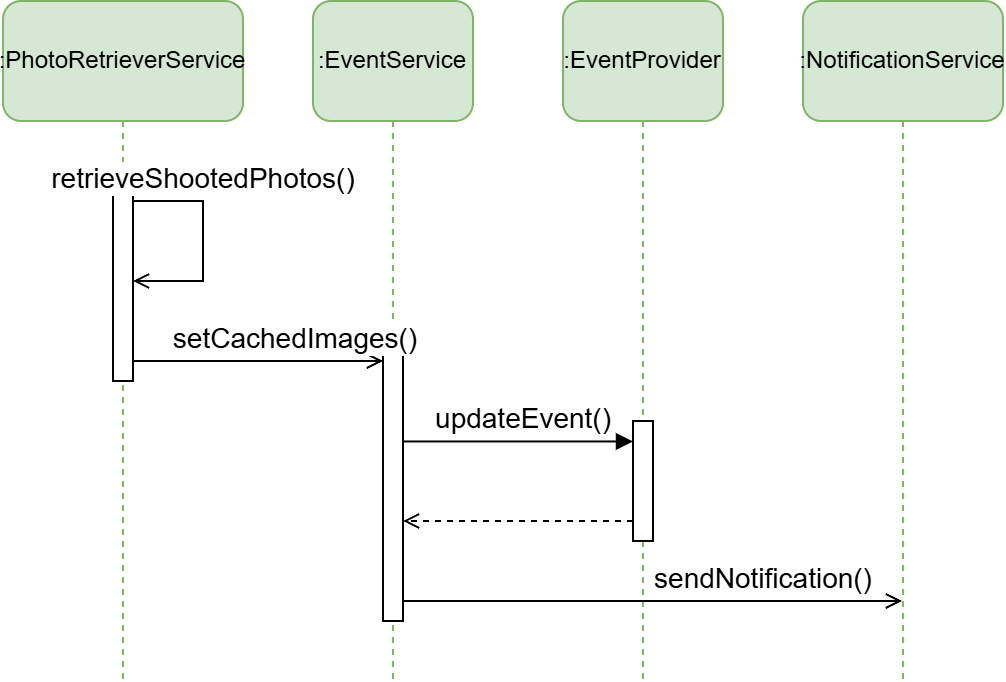
\includegraphics[height=0.45\textheight]{IIRecuperaImmagini.png}
    \caption{Interazione tra i componenti per il recupero delle immagini}
\end{figure}

Questa fase di conferma, oltre a garantire la trasparenza del servizio nei confronti dell’utente, 
riducendo il rischio di errori o caricamenti indesiderati, presenta anche vantaggi in termini di ottimizzazione delle prestazioni. 
\clearpage
Da un punto di vista normativo, la procedura di recupero e selezione automatica delle immagini è esplicitamente descritta nelle condizioni d’uso dell’applicazione, 
alle quali l’utente deve aderire con accettazione espressa prima di utilizzare il servizio. 
Tuttavia, la fase di conferma dell’utente non rappresenta un obbligo giuridico, 
poiché la responsabilità della pubblicazione di contenuti multimediali ricade sul soggetto che realizza la fotografia. 
In conformità con la normativa vigente in materia di tutela dell’immagine (art. 10 c.c. e artt. 96-97 della Legge n. 633/1941) e protezione dei dati personali (Regolamento UE 2016/679 – GDPR), 
chi scatta una fotografia è tenuto a ottenere il consenso delle persone ritratte prima di procedere alla sua pubblicazione.\\
\\
Come già affrontato nel capitolo precedente, le operazioni che coinvolgono la modifica di uno stesso componente del sistema 
sono soggette a vincoli di concorrenza per l’accesso alla risorsa di interesse. 
La conclusione di un evento condiviso tra più utenti potrebbe generare richieste simultanee per l’aggiunta di immagini associate a un medesimo evento. 
L’introduzione della fase di selezione introduce un ritardo nella fase di caricamento, 
dilatando la distribuzione temporale delle richieste e riducendo la probabilità di collisioni dovute a operazioni concorrenti sullo stesso elemento.
L’attesa della conferma dell’utente prevede infatti un ritardo fisiologico tra la fine dell’evento e l’effettivo caricamento delle immagini, 
contribuendo a distribuire le richieste nel tempo e limitando il rischio di congestione del server dovuta a operazioni simultanee su un singolo evento.\\
\\
Una volta completata la selezione da parte dell’utente, le immagini vengono inviate al server, che provvede al loro salvataggio e all’associazione con l’evento corrispondente.


\clearpage

\section{L'integrazione con il sistema}

A differenza dei dati tradizionalmente scambiati all’interno del sistema, i file multimediali presentano dimensioni significativamente superiori, 
con diversità che si manifestano su ordini di grandezza rilevanti. 
Un salvataggio di tali file nel flusso di dati standard, allineandoli agli elementi logici, 
comporterebbe un rallentamento generale delle operazioni e un impatto significativo sulle prestazioni complessive del sistema. 
Per questo motivo, è necessaria una gestione della memoria specificamente progettata per l’archiviazione e il recupero di contenuti multimediali.	\\
\\
Inoltre, Le dimensioni delle immagini e dei video influenzano direttamente il tempo di elaborazione e il volume delle richieste, 
aumentando il carico computazionale su tutti i componenti del sistema. 
In aggiunta, la possibilità di allegare più file a un singolo evento implica che i tempi di caricamento più elevati dei file multimediali 
possano prolungare sensibilmente la durata delle transazioni necessarie per la modifica degli eventi, incidendo sulla reattività del sistema.\\
\\
\clearpage
\subsection{La procedura di salvataggio}

La visualizzazione dei file multimediali riveste un'importanza secondaria rispetto ad altre funzionalità offerte dall'applicazione. 
Di conseguenza, è possibile accettare un maggiore tempo di caricamento, a condizione che ciò contribuisca a ridurre la latenza delle operazioni invece più rilevanti. 
Il salvataggio dei file multimediali direttamente nel database centrale comporterebbe un aumento significativo del volume delle richieste, 
determinando un maggiore impiego di risorse computazionali e un incremento dei tempi di caricamento. 
Questo fenomeno potrebbe incidere negativamente sulle prestazioni complessive del sistema, penalizzando l’esecuzione simultanea di altre operazioni.\\
\\
Per ottimizzare la gestione dei file multimediali, si adotta una distinzione della relazione tra l’oggetto logico e l'evento dai dati binari che lo compongono. 
In questo modo, la relazione tra il file e l’evento associato viene mantenuta indipendentemente dai dati binari che lo compongono. 
Una volta recuperati i riferimenti ai file multimediali associati all’evento in questione, sarà possibile ottenere poi i loro contenuti binari in un secondo momento, solo quando necessario.
Il modello del dominio illustrato in precedenza evidenzia la relazione logica tra gli eventi e i file associati (Photo).\\
\\
Considerando la necessità e la possibilità di archiviare i file multimediali su risorse differenti dal database centrale, 
è fondamentale individuare la soluzione più adatta alla loro persistenza. 
I principali servizi cloud per l’archiviazione di file multimediali si suddividono in tre categorie: Object Storage, File Storage e Block Storage.
Gli Object Storage gestiscono i file in un unico livello, con la possibilità di aggiungere metadati agli oggetti. 
A ciascun elemento viene associato un identificativo univoco che ne consente il recupero. 
L’accesso ai dati avviene tipicamente tramite API RESTful, che oltre ad offrire la possibilità di gestire i permessi, garantisce l’utilizzo su ampia scala. 
La presenza di un unico livello di indirizzamento permette una scalabilità pressoché illimitata, e un costo variabile in base alla quantità di dati memorizzati.
I File Storage organizzano i file in una struttura gerarchica di cartelle e sottocartelle, semplificando la gestione dei file e il controllo degli accessi. 
Oltre a facilitare un controllo ulteriore agli utenti, questa soluzione è compatibile con protocolli di accesso particolari. 
Tuttavia, la sua capacità e scalabilità, così come il costo effettivo, sono legati alla struttura dei file e alla capacità prevista dal piano selezionato.
Infine, i Block Storage gestiscono la memoria tramite la suddivisione dei dati in blocchi logici, salvati separatamente e ognuno dotato di identificativo univoco. 
Questa tecnologia offre elevate prestazioni per il recupero e la modifica dei dati, ma i costi aumentano all'incremento della quantità di dati presenti. 
La scalabilità è quindi limitata alla capacità assegnata al volume. Oltretutto, i costi sono elevati, particolarmente riguardo moli di grandi entità.\\
\\
Tra queste soluzioni, la categoria degli Object Storage risulta la più adatta alle esigenze del progetto di salvataggio dei file multimediali. 
La sua scalabilità illimitata consente di gestire grandi volumi di elementi con una ridotta interdipendenza tra loro. 
Inoltre, l’identificazione univoca di ciascun oggetto garantisce una rapida individuazione dei dati e un’efficiente risposta prestazionale a numerose richieste contemporanee.\\
\\
Nel contesto di Azure, il servizio di Object Storage fornito è rappresentato da Azure Blob Storage (ABS). 
ABS adotta un’organizzazione centrata su Container, entità logiche che raggruppano più file multimediali e introducono un livello di indirizzamento aggiuntivo. 
L’accesso in lettura ai dati avviene tramite protocollo API RESTful, con autenticazione per l’aggiunta di nuovi elementi. 
Per ogni evento viene creato un Container dedicato, contenente le immagini corrispondenti.\\
\\
Terminata la selezione dei file multimediali, prima dell’invio al server, i dispositivi client eseguono la compressione delle immagini, 
riducendo il consumo di banda e il volume dei dati totali trasmessi. 
Questa strategia consente di diminuire il carico computazionale sul server, migliorando l’efficienza complessiva del sistema.\\
\\
Il server, una volta ricevuta la richiesta, esegue una verifica dei permessi di accesso necessari e procede con il caricamento delle immagini nel Container associato all’evento. 
Al termine dell’operazione, il database viene aggiornato con i riferimenti ai nuovi file multimediali, e gli utenti vengono notificati della modifica avvenuta.\\
\\
La visualizzazione di un evento con immagini allegate comporta la richiesta parallela da parte delle singole immagini del dispositivo client verso ABS. 
Le immagini vengono identificate univocamente attraverso la combinazione dell’hash dell’immagine con quello del Container associato all’evento.\\
\\

\begin{figure}[h!]
    \centering
    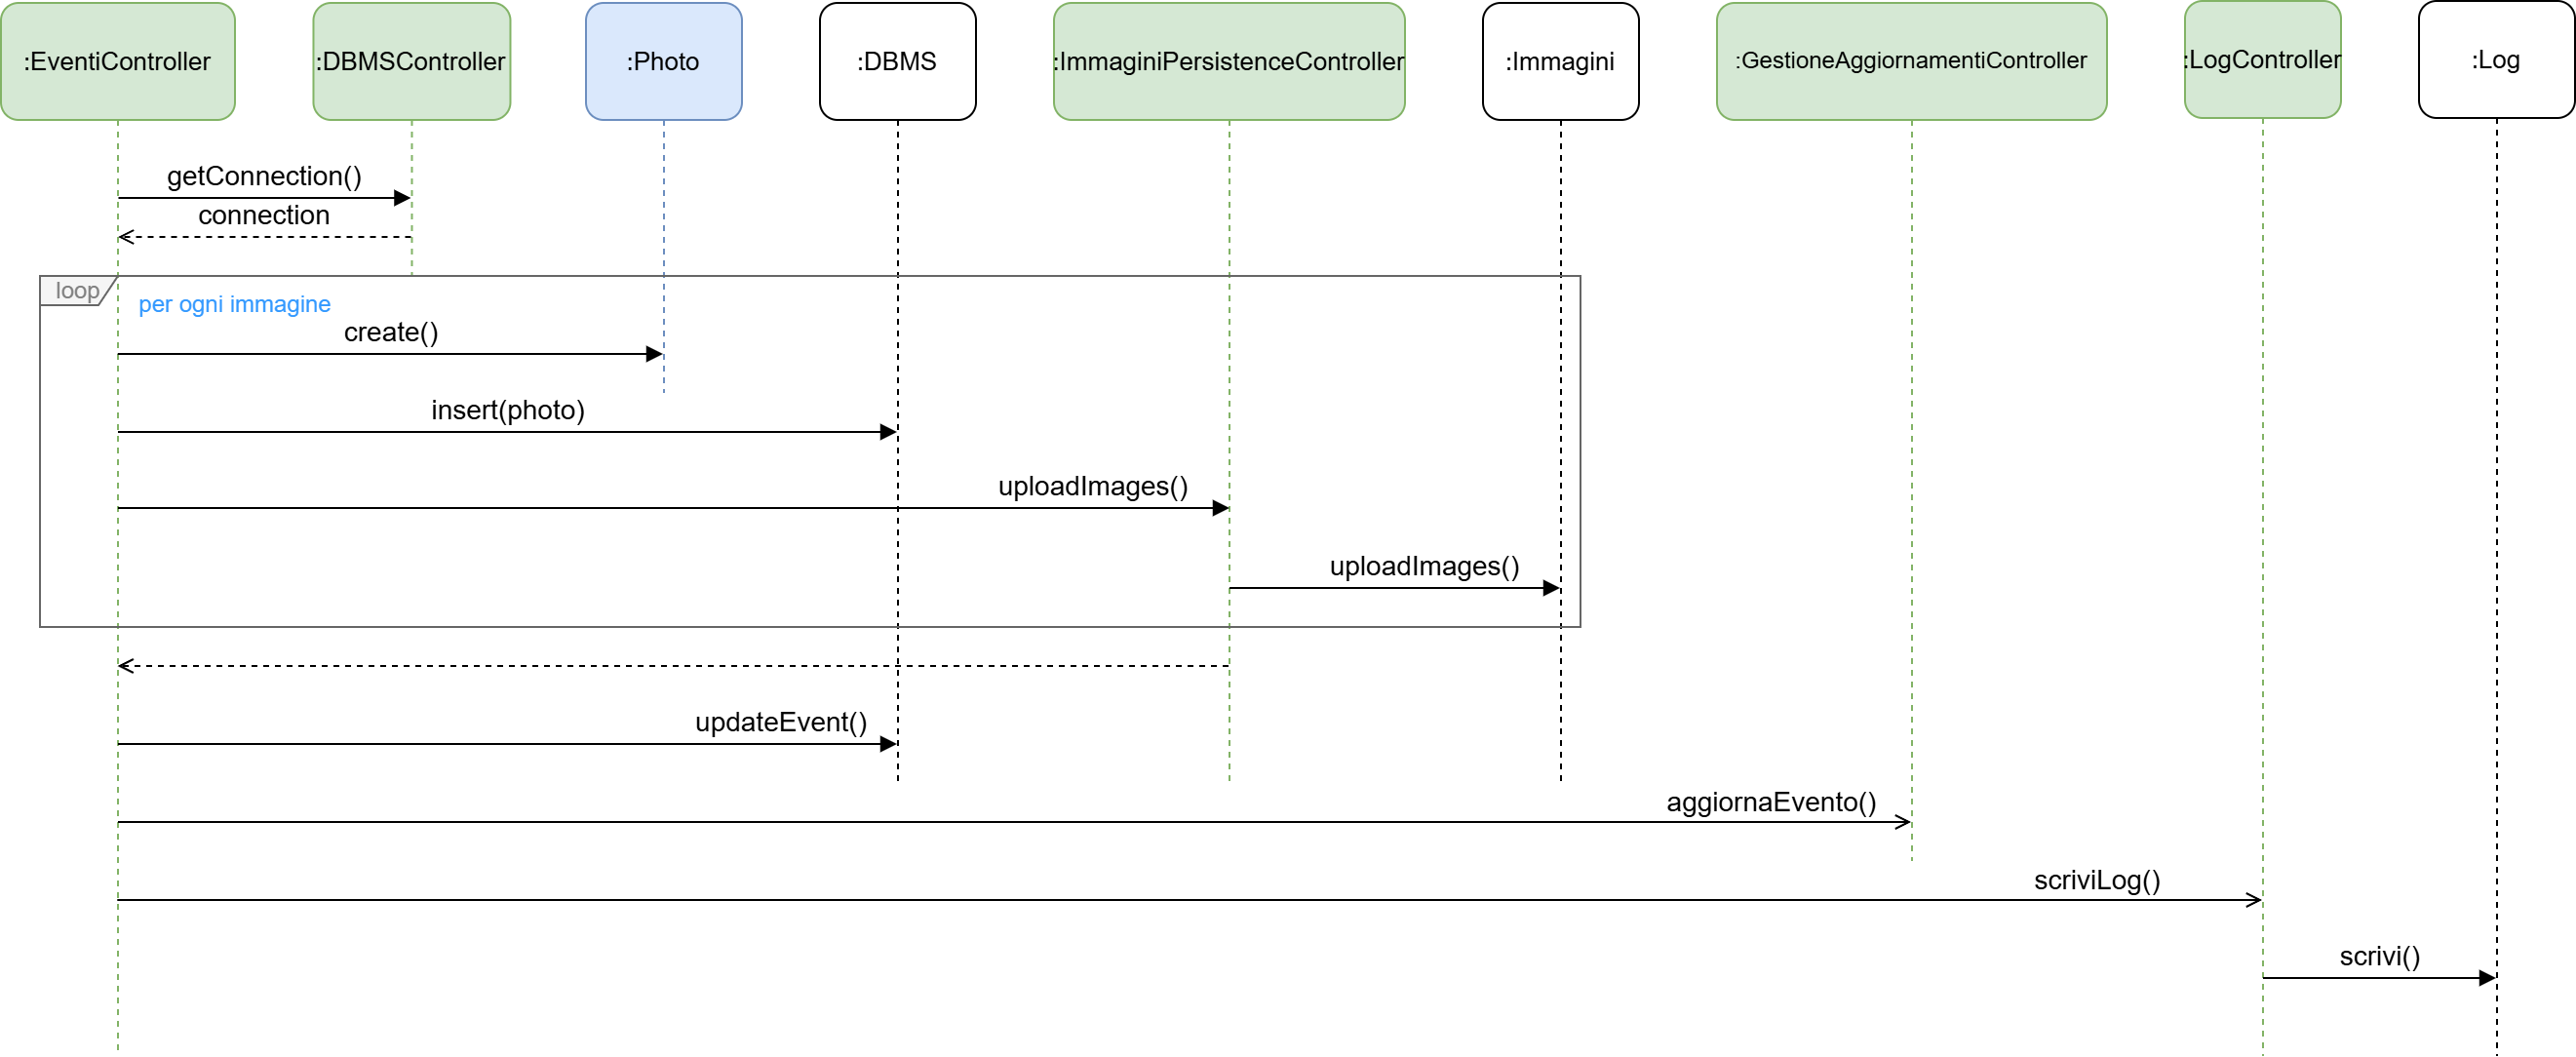
\includegraphics[width=\textwidth]{PIConfermaImmagini2.png}
    \caption{Interazione progettuale del server per il caricamento delle immagini }
\end{figure}

Tuttavia, l’accesso in lettura ai file multimediali in ABS risulta pubblico per impostazione predefinita, 
poiché la mancata definizione di ruoli comporta l’assenza di controlli espliciti sulle autorizzazioni delle richieste. 
Questo aspetto viene mitigato mediante l’uso di hash randomici sufficientemente lunghi, che riducono drasticamente la probabilità di collisione. 
Senza la conoscenza dell’hash corretto, un accesso non autorizzato alle immagini 
richiederebbe tentativi casuali estremamente numerosi nella speranza di trovare una combinazione corretta, rendendo un attacco altamente improbabile. 
Inoltre, anche in caso di compromissione di un hash, l’accesso sarebbe limitato a una singola immagine, senza fornire ulteriori informazioni sugli altri file memorizzati.

\clearpage

\subsection{La risoluzione ai problemi di concorrenza dovuti alla lunghezza delle richieste}

Il caricamento delle immagini dalle Azure Functions al Container associato all’evento rappresenta un'operazione relativamente onerosa in termini di tempo, 
soprattutto se confrontata con le altre operazioni eseguite dal sistema. 
La gestione delle connessioni tra il server e il database relazionale richiede dunque scelte di dominio e sviluppo mirate a garantire un uso ottimale delle risorse, 
minimizzando il tempo di blocco e migliorando l'efficienza complessiva.\\
\\
Un elemento centrale nel processo di invio dati è la gestione dell’hash dell’elemento Photo, che deve corrispondere al file caricato. 
L’hash viene generato al momento della creazione dell’oggetto, ma il suo salvataggio nel database avviene solo dopo il completamento del caricamento del file multimediale. 
Questa strategia evita operazioni di scrittura e cancellazione superflue, ottimizzando le prestazioni del sistema. 
Ne consegue che il momento della creazione dell’oggetto Photo deve essere logicamente distinto dal suo effettivo salvataggio nel database.

Per realizzare un’astrazione ad alto livello della relazione con il database, Entity Framework Core (EF Core) fornisce una rappresentazione logica degli elementi, 
mantenendo un collegamento con le relative controparti fisiche. 
Grazie a questa caratteristica, è possibile creare un oggetto senza doverlo immediatamente memorizzare, consentendo un controllo più preciso e immediato sul flusso dei dati.\\
\\
La relazione uno a molti tra gli eventi e le immagini è implementata mappando fisicamente  sugli oggetti Photo, 
i quali contengono un riferimento all’identificativo dell’evento associato. 
Al momento del salvataggio, viene modificata esclusivamente la tabella relativa a Photo; 
tuttavia, tale operazione implica un blocco in scrittura anche sull’oggetto Event. 
Ciò avviene poiché l’oggetto Event è coinvolto a livello logico, come dimostrato anche dalla presenza di una lista virtuale contenente le immagini associate tra i suoi attributi.\\
\\
Per migliorare l’efficienza del caricamento, la trasmissione dei file multimediali verso il Container avviene in parallelo, 
riducendo il tempo complessivo necessario per completare l’operazione. 
Tuttavia, l’inserimento immediato di ciascun oggetto Photo nel database al termine di ogni caricamento comporterebbe un rischio di conflitti sull’oggetto Event 
e un potenziale sovraccarico del database. Per mitigare questi problemi, 
gli oggetti logici Photo delle trasmissioni avvenute con successo vengono temporaneamente conservati in memoria per essere salvati successivamente  in un’unica operazione.\\
\\
L'inserimento simultaneo di tutti gli elementi Photo validi all'interno di una stessa transazione consente di ottimizzare l’impatto sul database, 
riducendo i tempi di blocco sull’oggetto Event e minimizzando il rischio di collisioni tra richieste concorrenti. 
Questo approccio garantisce una maggiore scalabilità e una gestione più efficiente delle risorse del sistema coinvolte.\\
\\

\begin{figure}[h!]
    \centering
    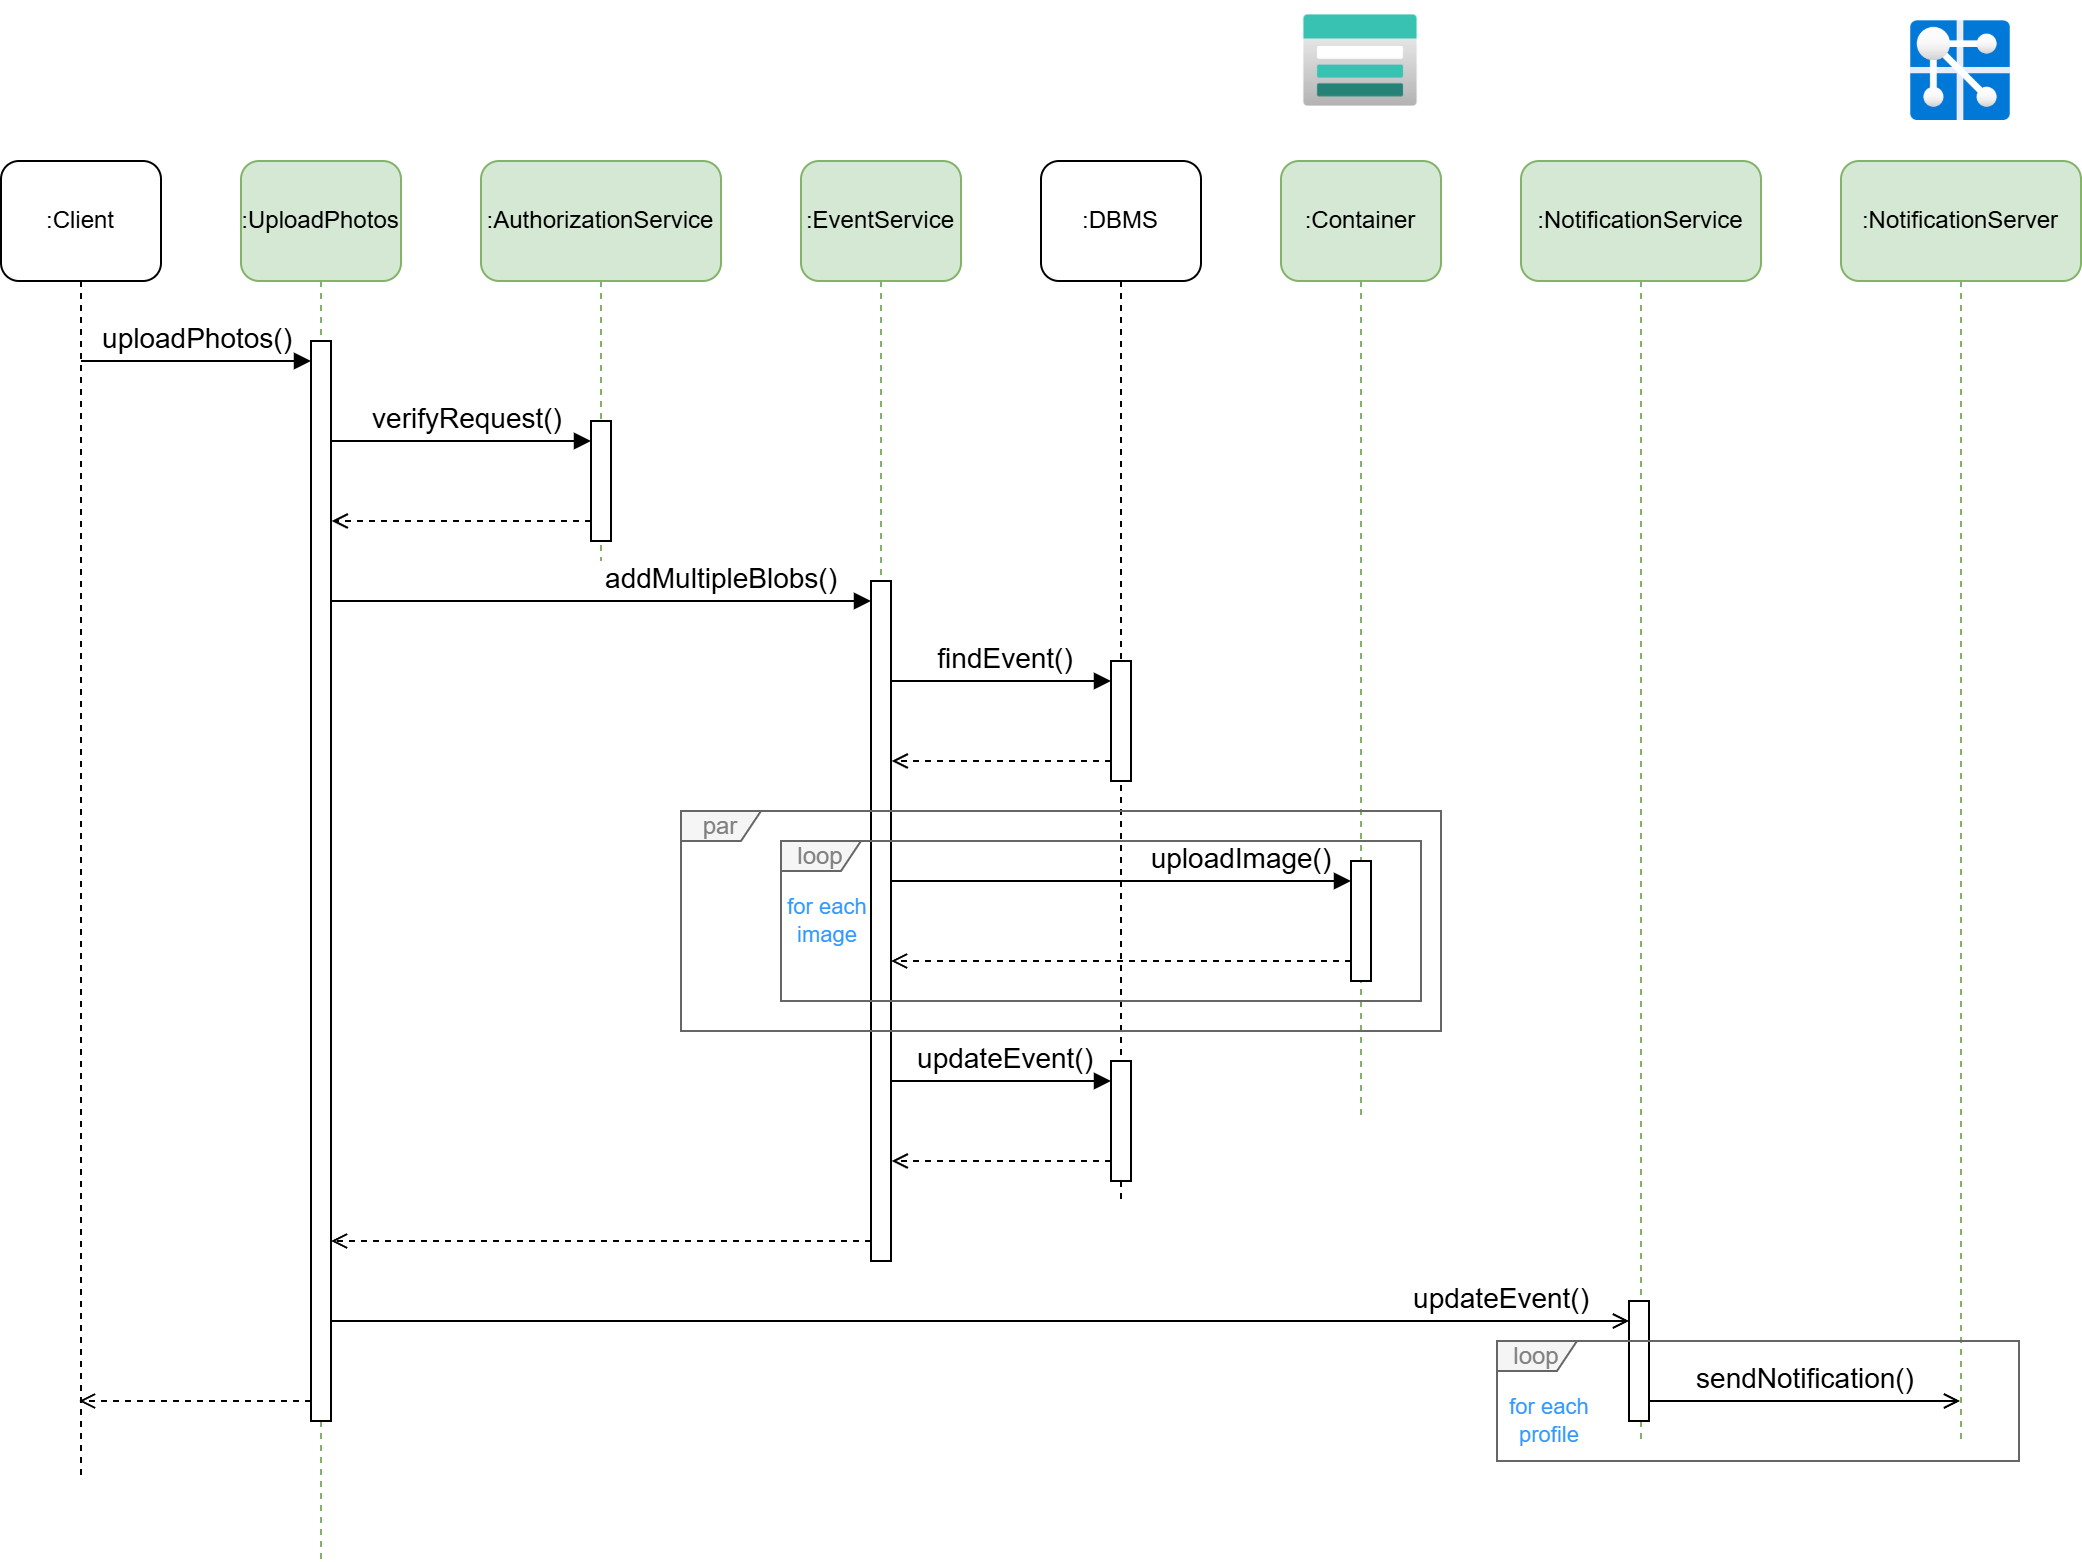
\includegraphics[width=\textwidth]{IICaricaImmagini.png}
    \caption{Interazione logica del server per il caricamento delle immagini }
\end{figure}

\clearpage
%
\chapter{Risultati}

\section{Velocità in lettura}

\begin{figure}[htbp]
    \begin{center}
        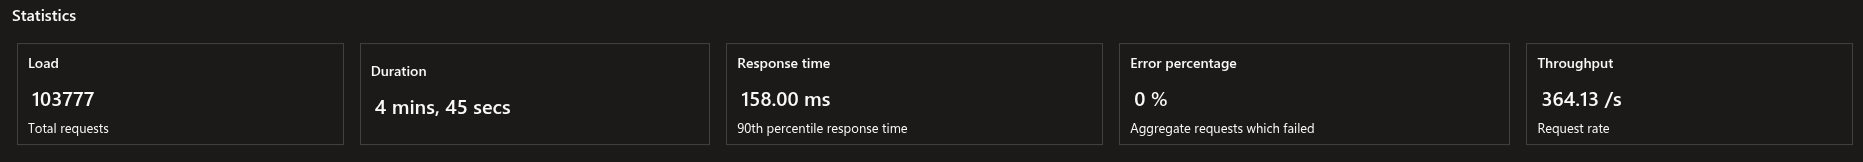
\includegraphics[width=\textwidth]{TestLettura1.png}
        \caption{158 ms su una media di 364 richieste al secondo}
    \end{center}
\end{figure}

\begin{figure}[htbp]
    \begin{center}
        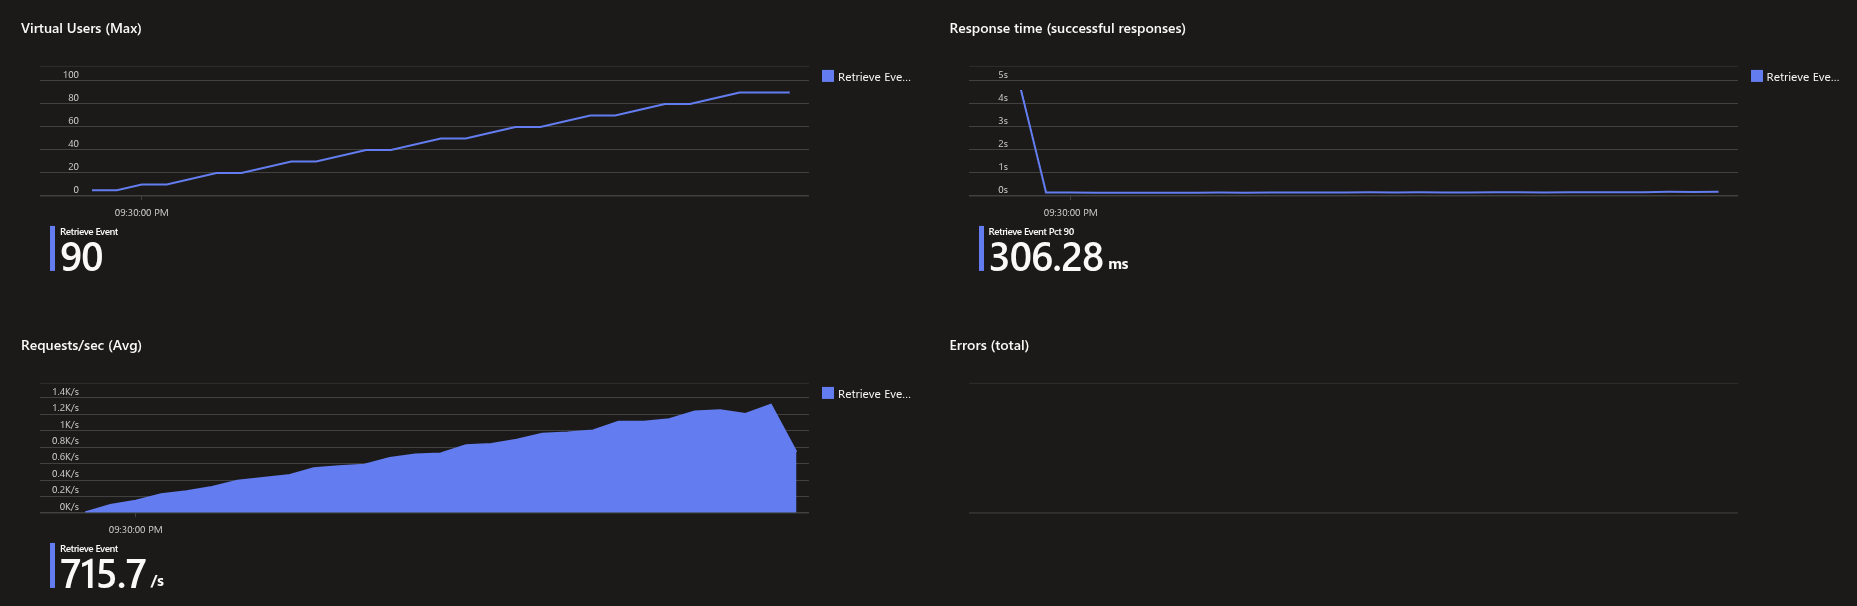
\includegraphics[width=\textwidth]{TestLettura2.png}
        \caption{il tempo di risposta non varia in base al numero di richieste}
    \end{center}
\end{figure}

\begin{figure}[htbp]
    \begin{center}
        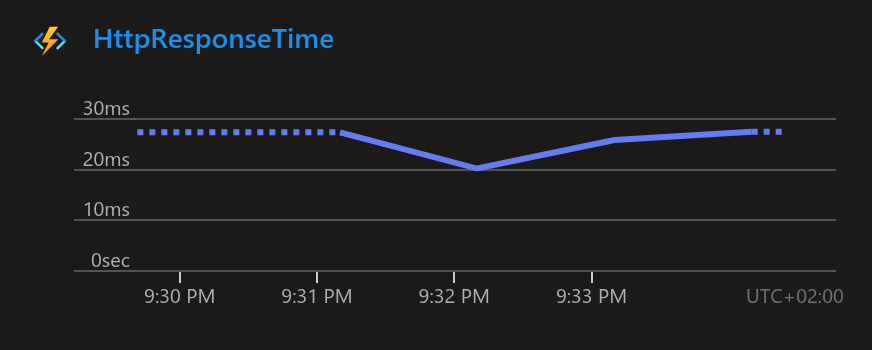
\includegraphics[width=\textwidth]{TestLettura3.png}
        \caption{Dettaglio della velocità senza tempo di trasmissione}
    \end{center}
\end{figure}
\clearpage
\section{Caricamento di immagini concorrenti}

\begin{figure}[htbp]
    \begin{center}
        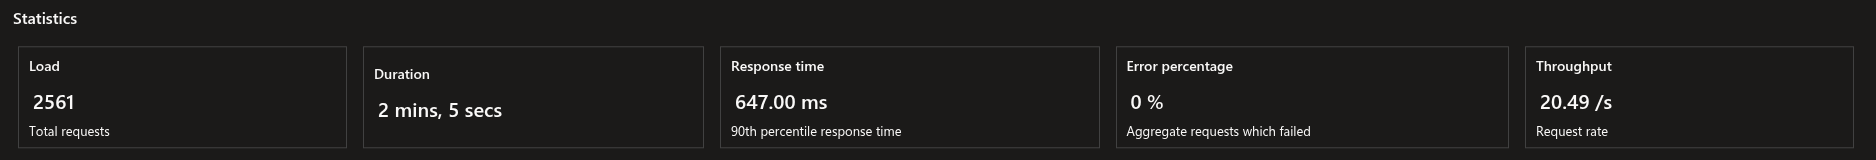
\includegraphics[width=\textwidth]{UploadImages1.png}
        \caption{2 MB di immagini in 600 ms 20 volte al secondo}  
    \end{center}
\end{figure}

\begin{figure}[htbp]
    \begin{center}
        \includegraphics[width=\textwidth]{UploadImages3.png}
        \caption{Andamento delle richieste}  
    \end{center}
\end{figure}

\begin{figure}[htbp]
    \begin{center}
        \includegraphics[width=\textwidth]{UploadImages2.png}
        \caption{Dettaglio della velocità richiesta dal server}
    \end{center}
\end{figure}


\clearpage
\chapter*{Conclusione}
\addcontentsline{toc}{chapter}{Conclusione}

\begin{figure}[htbp]
    \begin{center}
        \includegraphics[width=\textwidth]{ImplementazioneArchitettura.png}
        \caption{Grafico dell'architettura finale}
    \end{center}
\end{figure}
\clearpage

\section{Sviluppi futuri}
Gli sviluppi futuri potranno comprendere, in base a decisioni di marketing:
\begin{itemize}
    \item La visualizzazione degli impegni degli altri profili
    \item L'implementazione di una chat per ogni gruppo
    \item Sviluppo di strumenti utili all'organizzazione dei gruppi, quali:
          \begin{itemize}
              \item form per combinare le disponibilità reciproche
              \item appunti condivisi(liste della spesa o note su chi porta cosa)
              \item calcolo delle spese compiute da ciascun componente
          \end{itemize}
    \item La creazione di profili pubblici che possono essere seguiti
    \item La creazione di eventi pubblici
    \item Una funzionalità di ricerca degli eventi o dei profili pubblici
    \item Supporto alla gestione di prenotazione e organizzazione degli eventi, dalle liste di attesa alla vendita dei biglietti
    \item La possibilità per le aziende di gestire in locale il proprio server e i relativi dati
\end{itemize}
\clearpage

\chapter*{Fonti bibliografiche e sitografia}
\addcontentsline{toc}{chapter}{Fonti bibliografiche e sitografia}

Object Management Group, OMG Unified Modelling Language Version 2.5.1, December 2017, https://www.omg.org/spec/UML/2.5.1/PDF

\fancyhf{}
\end{document}